\documentclass[11pt]{report}

% ---------------------------------------------------------------------
% Packages
% ---------------------------------------------------------------------
\usepackage[a4paper,margin=2.5cm]{geometry}
\usepackage{amsmath,amssymb,amsthm}
\usepackage{listings}
\usepackage{xcolor}
\usepackage{tikz}
\usetikzlibrary{arrows.meta,positioning,fit,backgrounds,shapes.geometric,calc}
\usepackage{booktabs}
\usepackage{longtable}
\usepackage{array}
\usepackage{tabularx}
\usepackage{caption}
\usepackage{subcaption}
\usepackage{enumitem}
\usepackage{mdframed}
\usepackage{hyperref}
\usepackage{fancyhdr}
\usepackage{titlesec}
\usepackage{tcolorbox}
\tcbuselibrary{skins,breakable}

\hypersetup{
  colorlinks=true,
  linkcolor=blue!50!black,
  citecolor=blue!50!black,
  urlcolor=blue!50!black,
  bookmarksopen=true,
  pdftitle={shmap: Sketch-Based Long-Read Mapping --- Algorithm and Implementation Reference},
  pdfauthor={Reverse-engineered technical reference}
}

\pagestyle{fancy}
\fancyhf{}
\fancyhead[L]{\small\nouppercase{\leftmark}}
\fancyhead[R]{\small shmap algorithm reference}
\fancyfoot[C]{\thepage}
\renewcommand{\headrulewidth}{0.4pt}

% ---------------------------------------------------------------------
% Code listing styles
% ---------------------------------------------------------------------
\definecolor{codebg}{RGB}{247,247,250}
\definecolor{codeframe}{RGB}{200,200,210}
\definecolor{kwcolor}{RGB}{0,90,170}
\definecolor{strcolor}{RGB}{140,20,20}
\definecolor{cmtcolor}{RGB}{100,110,100}
\definecolor{numcolor}{RGB}{130,50,140}

\lstdefinestyle{cppstyle}{
  language=C++,
  backgroundcolor=\color{codebg},
  rulecolor=\color{codeframe},
  frame=single,
  framesep=4pt,
  basicstyle=\ttfamily\scriptsize,
  keywordstyle=\color{kwcolor}\bfseries,
  stringstyle=\color{strcolor},
  commentstyle=\color{cmtcolor}\itshape,
  numberstyle=\tiny\color{numcolor},
  numbers=left,
  numbersep=6pt,
  breaklines=true,
  breakatwhitespace=false,
  showstringspaces=false,
  tabsize=2,
  columns=fullflexible,
  captionpos=b,
}

\lstdefinestyle{rststyle}{
  backgroundcolor=\color{codebg},
  rulecolor=\color{codeframe},
  frame=single,
  framesep=4pt,
  basicstyle=\ttfamily\scriptsize,
  keywordstyle=\color{kwcolor}\bfseries,
  stringstyle=\color{strcolor},
  commentstyle=\color{cmtcolor}\itshape,
  numberstyle=\tiny\color{numcolor},
  numbers=left,
  numbersep=6pt,
  breaklines=true,
  breakatwhitespace=false,
  showstringspaces=false,
  tabsize=2,
  columns=fullflexible,
  captionpos=b,
  morekeywords={impl,pub,fn,struct,enum,match,let,mut,self,Self,while,for,if,else,return,use,mod,const,trait,where,dyn,as},
}

\lstdefinestyle{pseudostyle}{
  backgroundcolor=\color{white},
  basicstyle=\ttfamily\small,
  breaklines=true,
  breakatwhitespace=false,
  showstringspaces=false,
  columns=fullflexible,
  keywordstyle=\bfseries,
  morekeywords={function,procedure,return,if,then,else,end,for,in,while,do,break,continue,and,or,not},
}

% ---------------------------------------------------------------------
% Pseudocode box (no algorithm2e/algorithmic package available)
% ---------------------------------------------------------------------
\newtcolorbox{algobox}[2][]{
  breakable,
  enhanced,
  colback=gray!4,
  colframe=gray!55!black,
  boxrule=0.5pt,
  arc=1.5pt,
  left=6pt,right=6pt,top=4pt,bottom=4pt,
  fonttitle=\bfseries\sffamily\small,
  title={Algorithm: #2},
  #1
}

\newtcolorbox{notebox}[1][]{
  breakable, enhanced,
  colback=blue!4, colframe=blue!40!black,
  boxrule=0.4pt, arc=1.5pt,
  left=6pt,right=6pt,top=3pt,bottom=3pt,
  fonttitle=\bfseries\sffamily\small,
  title={Implementation note},
  #1
}

\newtcolorbox{bugbox}[1][]{
  breakable, enhanced,
  colback=red!4, colframe=red!45!black,
  boxrule=0.4pt, arc=1.5pt,
  left=6pt,right=6pt,top=3pt,bottom=3pt,
  fonttitle=\bfseries\sffamily\small,
  title={Known defect in the reference implementation},
  #1
}

\newcommand{\code}[1]{\texttt{\small #1}}
\newcommand{\field}[1]{\texttt{\small #1}}

% ---------------------------------------------------------------------
\title{
  \Huge\textbf{shmap}\\[0.3cm]
  \Large Sketch-Based Long-Read Mapping\\
  \large Algorithm and Implementation Reference\\[0.5cm]
  \normalsize From FracMinHash Sketching to Bucketed Seed-and-Extend Mapping
}
\author{Technical reference compiled from source analysis and a full independent re-implementation}
\date{\today}

\begin{document}

\maketitle

\begin{abstract}
\noindent
This document is a complete algorithmic and implementation reference for \textbf{shmap} (also
known as \emph{Map-SHmap} / \emph{sweepmap}), a sketch-based long-read mapper. It is written to
be sufficient, on its own, to re-implement the tool from scratch in any language: every data
structure, every formula, every loop invariant, and every edge case is specified precisely, with
excerpts from both the original C++ implementation and an independent Rust re-implementation
produced during the analysis that underlies this document. The exercise of producing a
line-for-line port surfaced several defects and dead code paths in the reference implementation;
these are documented explicitly (in ``Known defect'' boxes) so that a from-scratch implementer can
make an informed choice about whether to reproduce or correct them.

The document begins with the theoretical background required to understand the algorithm
(k-mers, canonical strands, minimizer-style sketching, FracMinHash / Mash-style sketching,
Jaccard and containment similarity, seed-and-extend mapping, longest increasing subsequence
chaining, and mapping-quality estimation), then describes the system architecture, then proceeds
module-by-module through the full implementation, and closes with complexity analysis, a full
end-to-end pseudocode listing, a CLI/parameter reference, and an appendix cataloguing every
discovered defect.
\end{abstract}

\tableofcontents

\chapter{Introduction}

\section{The long-read mapping problem}

Given a \emph{reference} sequence (or a set of reference segments, e.g.\ chromosomes/contigs)
$T = T_1, \dots, T_s$ over the alphabet $\Sigma = \{A, C, G, T\}$, and a \emph{query} read $P$
(typically $1$--$100+$\,kbp for long-read sequencing technologies such as PacBio HiFi or Oxford
Nanopore), the mapping problem is: find the location(s) $(i, [l, r))$ --- segment index $i$ and
half-open interval $[l, r) \subseteq [0, |T_i|)$ --- such that $T_i[l..r)$ is the region of the
reference that $P$ most likely originated from, together with a confidence score (mapping
quality, MAPQ).

This differs from \emph{alignment}: mapping only needs to find the correct region and strand, not
compute a base-level edit script (CIGAR). Mapping is the first, and usually the computational
bottleneck, phase of most long-read tools (minimap2, Winnowmap, MashMap, mapquik, and shmap all
separate mapping from an optional downstream alignment phase).

The naive solution --- align $P$ against every possible substring of $T$ with a full dynamic
program (edit distance / Smith--Waterman) --- costs $O(|T|\cdot|P|)$ per read and is many orders
of magnitude too slow for genome-scale references ($|T| \sim 10^9$--$10^{10}$) and
population-scale read sets ($10^5$--$10^7$ reads). All practical long-read mappers instead use a
\textbf{seed-and-extend} (or \emph{seed-chain-extend}) strategy: cheaply find a small number of
short, exact-matching anchors (\emph{seeds}) between $P$ and $T$, then use only the anchors'
positions --- not the sequence content --- to decide where $P$ came from.

\section{shmap's approach in one paragraph}

shmap represents both the reference and each read as a \textbf{FracMinHash sketch}: a
size-proportional, hash-thresholded subset of the sequence's $k$-mers (Chapter~\ref{ch:theory}
develops this precisely). Reference $k$-mers are indexed once into a hash table mapping
$k$-mer hash $\to$ list of reference positions. For each read, its own sketch is grouped into
\emph{seeds} (rarest $k$-mers first) and matched against the index; matches are accumulated into
overlapping, fixed-length \emph{buckets} along each reference segment. A cheap, provably-safe
\emph{seed heuristic} upper bound is used to prune buckets that cannot possibly beat the current
best candidate before any expensive refinement is attempted on them. Buckets that survive pruning
are refined with an exact two-pointer / sliding-window sweep (or, in alternate configurations, a
longest-common-subsequence chain) to produce a Jaccard or containment similarity score; the best
and second-best surviving mappings are used to compute a mapping-quality estimate; and the result
is emitted in PAF format with a rich set of custom diagnostic tags.

Two design choices set shmap apart from more familiar tools like minimap2:
\begin{enumerate}
  \item \textbf{FracMinHash sketching instead of minimizer windows.} Rather than picking one
    minimal-hash $k$-mer per sliding window (a \emph{minimizer} scheme), shmap keeps every k-mer
    whose hash falls below a fixed fraction of the hash space. This makes sketch size
    \emph{proportional to sequence length} with a tunable ratio $r$ (flag \code{-r}), rather than
    proportional to (length / window size); see \S\ref{sec:fracminhash-vs-minimizer}.
  \item \textbf{Score-bound-driven bucket pruning instead of chaining every anchor.} Instead of
    running a full co-linear chaining dynamic program over every seed hit (as minimap2 does),
    shmap only ever considers small, fixed-geometry \emph{buckets} of the reference, and prunes
    the overwhelming majority of them using a cheap closed-form upper bound on the score they
    could possibly achieve, before doing any real work on them. This is the ``SH'' (seed
    heuristic) in the tool's Map-SHmap name.
\end{enumerate}

\section{How to use this document}

The chapters are ordered so that a reader with no prior background in sketch-based mapping can
start at Chapter~\ref{ch:theory} and, by the time they reach the per-module chapters
(Chapters~\ref{ch:sketching}--\ref{ch:scoring}), already understand \emph{why} every formula and
data structure exists, not just \emph{what} it computes. Each per-module chapter gives:
\begin{itemize}[nosep]
  \item the exact input/output contract of every function (types, units, invariants assumed and
    guaranteed);
  \item a boxed pseudocode listing that is language-independent and directly implementable;
  \item excerpts of the original C++ (from the \texttt{shmap} repository, files under
    \texttt{src/}) and of an independent Rust re-implementation, side by side, wherever the exact
    bit-level or control-flow behavior matters;
  \item worked numeric examples for the trickiest arithmetic (bucket geometry, the FracMinHash
    rolling hash, the seed-heuristic bound);
  \item boxed notes on defects discovered by cross-checking the two implementations against each
    other and against the algorithm's own stated invariants --- several of which are not merely
    cosmetic (Chapter~\ref{ch:defects} collects all of them with full detail).
\end{itemize}

Chapter~\ref{ch:end-to-end} then reassembles every module into one top-to-bottom pseudocode
listing of the per-read mapping routine, which is the single most useful reference for a
from-scratch implementation. Chapter~\ref{ch:appendix} collects notation, a symbol table, and a
condensed algorithm index for quick lookup while implementing.

\chapter{Theoretical Background}
\label{ch:theory}

This chapter develops, from first principles, every theoretical tool shmap relies on. No prior
familiarity with sketch-based mapping is assumed.

\section{$k$-mers}

A \textbf{$k$-mer} is a contiguous substring of length $k$ of a DNA sequence. A sequence $S$ of
length $n$ over $\Sigma=\{A,C,G,T\}$ has exactly $n-k+1$ $k$-mers (for $n \ge k$), one starting at
each position $i \in [0, n-k]$: $S[i \mathinner{.\,.} i{+}k)$.

$k$-mers are the atomic unit of comparison in almost all modern sequence analysis: instead of
comparing sequences character-by-character (which is what alignment does, and is expensive),
tools compare the \emph{sets} of $k$-mers two sequences share. Two sequences that share many
$k$-mers are likely to be similar/overlapping/from the same genomic locus; two that share almost
none are likely unrelated. This is the basis of alignment-free sequence comparison.

Two design parameters govern how well $k$-mers work as a similarity proxy:
\begin{itemize}
  \item If $k$ is too small, $k$-mers recur very frequently by chance alone (there are only
    $4^k$ distinct $k$-mers; for $k=8$ that is $65{,}536$, tiny compared to a genome of $10^9$
    bases), so a shared $k$-mer carries little evidence of true homology.
  \item If $k$ is too large, a single sequencing error (common in long reads, particularly Oxford
    Nanopore data, at rates of $1$--$15\%$ depending on chemistry) destroys every $k$-mer that
    overlaps it (up to $k$ of them), so real matches are missed.
\end{itemize}
shmap's default is $k=15$ (flag \code{-k}), with typical experiments in the codebase's own
evaluation harness sweeping $k \in \{17,19,\dots,33\}$.

\subsection{Canonical $k$-mers and strand}
\label{sec:canonical-kmers}

DNA is double-stranded, and a sequencing read may originate from either strand, with no way to
know which \emph{a priori}. A $k$-mer $x$ occurring on the forward strand of the reference is
identical to the \textbf{reverse complement} of $x$ occurring on the reverse strand at the
mirrored position. To make $k$-mer matching strand-agnostic, essentially every tool in this space
computes, for each $k$-mer window, both:
\begin{itemize}[nosep]
  \item the forward-strand hash $h_{fw}$, and
  \item the reverse-complement hash $h_{rc}$ (i.e., the hash of the reverse complement of the
    same window),
\end{itemize}
and uses a canonical combination of the two (commonly $\min(h_{fw}, h_{rc})$, or, as shmap does,
$h_{fw} \oplus h_{rc}$ --- see \S\ref{sec:fracminhash-hash}) as the $k$-mer's identity, plus a
single bit recording which strand ``won'' so that downstream code can recover orientation.

\section{Hashing $k$-mers, and rolling hashes}
\label{sec:rolling-hash}

Because a sequence of length $n$ has $O(n)$ overlapping $k$-mers, naively hashing each one from
scratch costs $O(nk)$. A \textbf{rolling hash} instead updates the previous window's hash in
$O(1)$ to obtain the next window's hash, giving $O(n)$ total. The general recurrence for a
polynomial or XOR-based rolling hash removes the outgoing base's contribution and adds the
incoming base's contribution:
\[
  h_{i+1} = f(h_i, \, \text{out\_base} = S[i], \, \text{in\_base} = S[i+k])
\]
shmap uses an XOR/rotate rolling hash (not a polynomial one); the exact recurrence, including the
reverse-complement side, is derived in \S\ref{sec:fracminhash-hash}.

\section{Sketching: reducing $k$-mer sets to a manageable, comparable size}

Even with an efficient rolling hash, a set of $O(n)$ $k$-mers per sequence is too large to
compare pairwise across, e.g., every read against a whole genome. \textbf{Sketching} techniques
subsample the $k$-mer set down to a small representative subset, in a way that lets similarity
between two sequences be \emph{estimated} from the subsets alone, with a distortion (approximation
error) that shrinks as the subset grows.

\subsection{Minimizer schemes}
\label{sec:minimizers}

The most widely used sketching scheme (used by minimap2, most short-read aligners' seed indices,
Winnowmap, etc.) is the \textbf{minimizer}: slide a window of $w$ consecutive $k$-mers along the
sequence, and keep only the $k$-mer with the smallest hash value in each window (ties broken by
position or a secondary key). This guarantees:
\begin{itemize}[nosep]
  \item \textbf{Bounded density:} at most $2/(w+1)$ of all $k$-mers are ever selected (in
    expectation, for a uniform hash), giving a sketch size proportional to $n/w$.
  \item \textbf{Window guarantee:} any window of $w$ consecutive $k$-mers has \emph{at least one}
    selected minimizer, so no region of the sequence is left completely unsampled --- important
    for finding short matches / handling indels robustly.
\end{itemize}
The window guarantee is minimizers' main strength; their main weakness is that the selected set is
sensitive to single-base edits near a window boundary (a phenomenon studied extensively in the
minimizer/syncmer literature), and that sketch size is governed by $w$, not by a similarity-space
quantity directly.

\subsection{MinHash}
\label{sec:minhash}

An older, different sketching idea (Broder, 1997) underlies Mash and sourmash. Given a hash
function $h$ assumed to distribute $k$-mers uniformly over $[0, H_{\max}]$, the \textbf{MinHash
sketch} of a $k$-mer set $A$ of size $n$ keeps only the $n$ smallest-hash elements for a
fixed target sketch size (\emph{bottom-$n$ sketch}), or equivalently the single minimum hash
value repeated over many independent hash functions (\emph{classic MinHash}). The key theoretical
result is:
\[
  \Pr[\min h(A) = \min h(B)] = \frac{|A \cap B|}{|A \cup B|} = J(A,B)
\]
i.e., the probability that two sets' minimum hashes coincide equals their \textbf{Jaccard
similarity}. Averaging this indicator over $m$ independent hash functions (or, equivalently,
comparing the $m$ smallest of a single hash function's outputs) gives an unbiased estimator of
$J(A,B)$ with standard error $O(1/\sqrt{m})$.

MinHash's practical drawback for genomic sketching: a fixed-size bottom-$n$ sketch of a short
sequence and of a long sequence look the same size, so a short sequence's sketch is a much denser
(and hence unrepresentative, if $n$ is not scaled per-sequence) sample of its $k$-mers. This
motivates \textbf{FracMinHash}.

\subsection{FracMinHash (``Mash Screen'' / scaled MinHash)}
\label{sec:fracminhash-theory}

\textbf{FracMinHash} (used by Mash Screen, sourmash's ``scaled'' sketches, and shmap) fixes not a
sketch \emph{size} but a hash-space \textbf{fraction} $r \in (0,1]$ (shmap's flag \code{-r},
default $0.05$): a $k$-mer with hash $h$ is kept in the sketch iff
\[
  h \le r \cdot H_{\max}
\]
where $H_{\max}$ is the maximum possible hash value (for a 64-bit hash, $H_{\max}=2^{64}-1$).
Because $h$ is (assumed) uniformly distributed, this keeps, in expectation, a fraction $r$ of all
$k$-mers, so \textbf{sketch size scales linearly with sequence length}: $|\text{sketch}(S)|
\approx r\cdot(|S|-k+1)$, for any $|S|$. This is the key advantage over both fixed-size MinHash
and (to a lesser extent) minimizers: one parameter $r$ controls sampling density uniformly across
sequences of any length, and, unlike bottom-$n$ MinHash, two FracMinHash sketches computed with
the \emph{same} threshold are directly comparable set-theoretically (their union/intersection
correspond exactly to the union/intersection of the full $k$-mer sets restricted to the
sub-threshold region) --- no renormalization needed.

\paragraph{Jaccard and containment estimation.} For two sketches $\hat A = A \cap [0, rH_{\max}]$
and $\hat B = B \cap [0, rH_{\max}]$ built with the \emph{same} threshold,
\[
  \widehat{J(A,B)} = \frac{|\hat A \cap \hat B|}{|\hat A \cup \hat B|}
  \qquad\text{estimates}\qquad
  J(A,B)=\frac{|A\cap B|}{|A \cup B|},
\]
and, when $|A| \ll |B|$ (e.g.\ $A$ a read, $B$ the whole genome) the more relevant
\textbf{containment index}
\[
  C(A, B) = \frac{|A \cap B|}{|A|}
\]
(``what fraction of the read's $k$-mers are found somewhere in the reference'') is estimated
directly (without needing to also estimate $|A \cup B|$) as
\[
  \widehat{C(A,B)} = \frac{|\hat A \cap \hat B|}{|\hat A|}.
\]
shmap's two headline metrics, \code{Containment} and \code{Jaccard} (CLI flag \code{-m}), are
exactly these two estimators, computed not over the whole reference but over a small candidate
\emph{bucket} region (Chapter~\ref{ch:scoring}); shmap additionally offers two alternative,
bucket-native metrics (\code{bucket\_SH}, \code{bucket\_LCS}) discussed in
\S\ref{sec:metric-variants}.

\subsection{FracMinHash vs.\ minimizers, concretely}
\label{sec:fracminhash-vs-minimizer}

\begin{center}
\begin{tabular}{@{}p{4cm}p{5.4cm}p{5.4cm}@{}}
\toprule
 & \textbf{Minimizer ($w$-window)} & \textbf{FracMinHash (ratio $r$)} \\
\midrule
Sketch size & $\approx 2n/(w{+}1)$ & $\approx rn$ \\
Coverage guarantee & every $w$-window has $\ge 1$ selected $k$-mer & none: a long low-hash-density
  stretch can (rarely) be unsampled \\
Comparable across lengths & only if $w$ fixed and sequences aligned to the same coordinate frame
  & yes, directly, by construction \\
Used by & minimap2, Winnowmap, most short-read aligners & Mash Screen, sourmash, \textbf{shmap} \\
\bottomrule
\end{tabular}
\end{center}

shmap explicitly favors the containment/Jaccard-estimation cleanliness of FracMinHash over
minimizers' coverage guarantee; its seed-heuristic pruning (\S\ref{sec:seed-heuristic-theory}) is
in fact a direct consequence of working in FracMinHash's clean estimation framework.

\section{Seed-and-extend / seed-chain-extend mapping}
\label{sec:seed-extend}

Given sketches of $P$ (the read) and $T$ (the reference), the generic mapping pipeline is:
\begin{enumerate}
  \item \textbf{Seed:} find every position where a $k$-mer of $P$'s sketch also occurs in $T$'s
    sketch (a \emph{hit}); a hit is a pair (position in $P$, position in $T$).
  \item \textbf{Chain / cluster:} group hits that are roughly co-linear (i.e., consistent with one
    contiguous alignment: as position-in-$P$ increases, position-in-$T$ increases by a
    comparable amount, same strand) into candidate regions.
  \item \textbf{Score / extend:} for each candidate region, compute a similarity score (or, in
    tools that go further, a base-level alignment) and report the best (and, for mapping quality,
    second-best) candidate.
\end{enumerate}
Tools differ enormously in step 2. minimap2 runs an $O(N \log N)$ or $O(N^2)$ (bounded) dynamic
program over all $N$ hits to find the highest-scoring chain of co-linear anchors (\emph{co-linear
chaining}). shmap instead partitions the reference into fixed-geometry, overlapping
\textbf{buckets} (a form of coarse, position-only clustering, described in
Chapter~\ref{ch:bucketing}) and scores whole buckets rather than chaining individual hits --- far
cheaper, at the cost of being less precise about the exact alignment boundary (which shmap does
not need, since it is a mapper, not an aligner).

\section{Co-linear chaining via Longest Increasing / Common Subsequence}
\label{sec:lis-theory}

One of shmap's four scoring metrics, \code{bucket\_LCS} (\S\ref{sec:metric-variants}), scores a
candidate bucket by the length of the \textbf{longest common subsequence} (LCS) between the order
hits occur in $P$ and the order they occur in $T$ within the bucket. Because both sequences here
are permutations of (a subset of) the same multiset of positions-in-$P$, ``LCS'' reduces to
\textbf{longest increasing subsequence} (LIS) of the sequence of $P$-positions visited in
increasing $T$-order: a long increasing run means many hits are mutually co-linear (consistent
with one real alignment on one strand); a long \emph{decreasing} run means many hits are
co-linear on the \emph{other} strand. shmap computes both (forward and reverse) and takes the max
(\S\ref{sec:lcs-implementation}).

\paragraph{Patience-sorting LIS algorithm.} The classic $O(n\log n)$ algorithm for LIS length
(not full reconstruction) processes the sequence left to right, maintaining an array
$\mathit{tails}$ where $\mathit{tails}[i]$ is the smallest possible tail value of any increasing
subsequence of length $i{+}1$ seen so far. For each new value $x$: binary-search $\mathit{tails}$
for the first entry $\ge x$; if none exists, append $x$ (extends the longest run found so far by
one); otherwise overwrite that entry with $x$ (keeps the same achievable lengths but with a
smaller, more extensible tail). The final array length is the LIS length. This is exactly the
algorithm shmap's \code{lcs\_get\_lis} implements (\S\ref{sec:lcs-implementation}).

\section{The seed heuristic: a provable upper bound for cheap pruning}
\label{sec:seed-heuristic-theory}

This is the theoretical core that gives Map-SHmap its name and its main performance advantage
over exhaustively scoring every candidate region.

Consider a read sketch of size $m = |\hat P|$ (its FracMinHash sketch cardinality). Seeds are
consumed \emph{rarest-first} (Chapter~\ref{ch:seeding}) up to some budget $S \le m$ seeds. For any
candidate bucket, define:
\begin{itemize}[nosep]
  \item $\mathit{seeds}$ = number of seed \emph{occurrences} (counting multiplicity in $P$) that
    have been consumed and attributed to this bucket so far (an occurrence is attributed to a
    bucket the moment its position is examined --- whether or not the reference actually has a
    hit there);
  \item $\mathit{matches}$ = number of those occurrences that \emph{did} find a hit landing inside
    this bucket.
\end{itemize}
Necessarily $\mathit{matches} \le \mathit{seeds} \le m$ (a seed occurrence can match at most once
per bucket, and only $\mathit{seeds}\le m$ occurrences from the read have been consumed at all).
Define the \textbf{seed-heuristic score}
\[
  h_{\mathrm{seed}}(m, \mathit{seeds}, \mathit{matches}) \;=\; 1 - \frac{\mathit{seeds} -
  \mathit{matches}}{m}.
\]

\begin{quote}
\textbf{Claim.} $h_{\mathrm{seed}}$ is a non-increasing function of $\mathit{seeds}$ for fixed
$\mathit{matches}$, and an upper bound on the true containment score
$C = \mathit{matches}_{\mathrm{final}} / m$ that this bucket could achieve \emph{even if every
remaining, not-yet-consumed seed occurrence in $P$ also matched inside this bucket}.
\end{quote}

\emph{Why.} At most $m$ total seed occurrences exist; $\mathit{seeds}-\mathit{matches}$ of the
ones examined so far are \emph{known misses} for this bucket (an occurrence was consumed and did
\emph{not} land in this bucket). Even in the best possible case --- every one of the
$m-\mathit{seeds}$ not-yet-examined occurrences turns out to match this bucket too --- the final
match count can be at most $m - (\mathit{seeds}-\mathit{matches})$ (total occurrences minus known
misses), giving final containment score at most
$\bigl(m-(\mathit{seeds}-\mathit{matches})\bigr)/m = h_{\mathrm{seed}}$. Since known misses only
ever accumulate (both $\mathit{seeds}$ and $\mathit{seeds}-\mathit{matches}$ are non-decreasing as
more occurrences are examined), $h_{\mathrm{seed}}$ can only decrease or stay the same as more
seeds are consumed for a fixed bucket --- it is a monotonically tightening upper bound.

\paragraph{Pruning rule.} If, after extending a bucket with more seed occurrences,
$h_{\mathrm{seed}} < \theta$ for the current acceptance threshold $\theta$ (or the current
best-known score, whichever is the active bound), the bucket is \emph{guaranteed} to be unable to
reach $\theta$ no matter how the remaining seeds resolve, and can be discarded \emph{without
computing its actual score}. This is what makes shmap fast: the overwhelming majority of
candidate buckets a repetitive genome generates are eliminated by this $O(1)$-per-check bound
long before the $O(\text{bucket size})$ refinement sweep (Chapter~\ref{ch:scoring}) would ever
run on them. Chapter~\ref{ch:pruning} gives the exact incremental algorithm
(\code{seed\_heuristic\_pass}) that extends a bucket with just enough additional seeds to either
prove it's prunable or exhaust all seeds, at the smallest possible cost.

\section{Mapping quality (MAPQ)}
\label{sec:mapq-theory}

A mapper is rarely certain a single location is correct, especially in repetitive genomic regions
where a read may score similarly against several loci. \textbf{MAPQ} (following the SAM/PAF
convention, an integer typically in $[0,60]$, though PAF's own histrionic convention allows $255$
for ``unavailable'') encodes, on a Phred-like scale, the mapper's confidence that the reported
best location is correct. The general recipe used by essentially all mappers (originating with
MAQ/BWA, and reused with variations by minimap2 and shmap) is:
\begin{enumerate}[nosep]
  \item Find the best-scoring candidate location, score $f_1$.
  \item Find the best-scoring candidate location that is not simply a restatement of the same
    location (typically: does not overlap the first by more than some fraction), score $f_2\le
    f_1$.
  \item If $f_1$ and $f_2$ are close, the read could plausibly have come from either place ---
    report low confidence. If $f_2$ is much worse than $f_1$ (or no second candidate exists at
    all), report high confidence.
\end{enumerate}
shmap's concrete formula, and the specific (somewhat unusual, all-or-nothing rather than smoothly
graduated) way it implements step 3, is given in full in Chapter~\ref{ch:mapq}, including a
discussion of two alternative formulas the original source retains, commented out, as evidence of
in-progress tuning.

\section{Summary of the theoretical pipeline}

Putting the pieces together, shmap's high-level strategy is: \emph{FracMinHash sketch both sides
for length-proportional, directly-comparable $k$-mer subsets; index the reference sketch once;
for each read, seed rarest-$k$-mer-first against the index; accumulate hits into cheap,
overlapping positional buckets; use the seed-heuristic upper bound to discard almost all buckets
for a few arithmetic operations each; refine survivors with an exact sliding-window Jaccard/
containment sweep (or an LCS-based chain score); and report the best two candidates' scores as a
MAPQ estimate.} Chapter~\ref{ch:architecture} now turns this into the concrete system
architecture, and the chapters that follow specify every step precisely enough to implement.

\chapter{General Architecture}
\label{ch:architecture}

\section{Two phases: indexing and mapping}

shmap's execution splits into two clearly separated phases, run once per invocation:

\begin{enumerate}
  \item \textbf{Indexing phase} (Chapter~\ref{ch:indexing}): read the reference FASTA once,
    FracMinHash-sketch every segment, and build a hash map from $k$-mer hash to the list of
    reference positions (\emph{hits}) sharing that hash. This is done once regardless of how many
    reads are mapped afterward.
  \item \textbf{Mapping phase} (Chapters~\ref{ch:seeding}--\ref{ch:scoring},
    reassembled end-to-end in Chapter~\ref{ch:end-to-end}): stream the read FASTA/FASTQ one record
    at a time; for each read, sketch it, seed it against the index, bucket the hits, prune buckets
    with the seed heuristic, refine survivors, compute MAPQ from the best two survivors, and emit
    one PAF line.
\end{enumerate}

\begin{figure}[htbp]
\centering
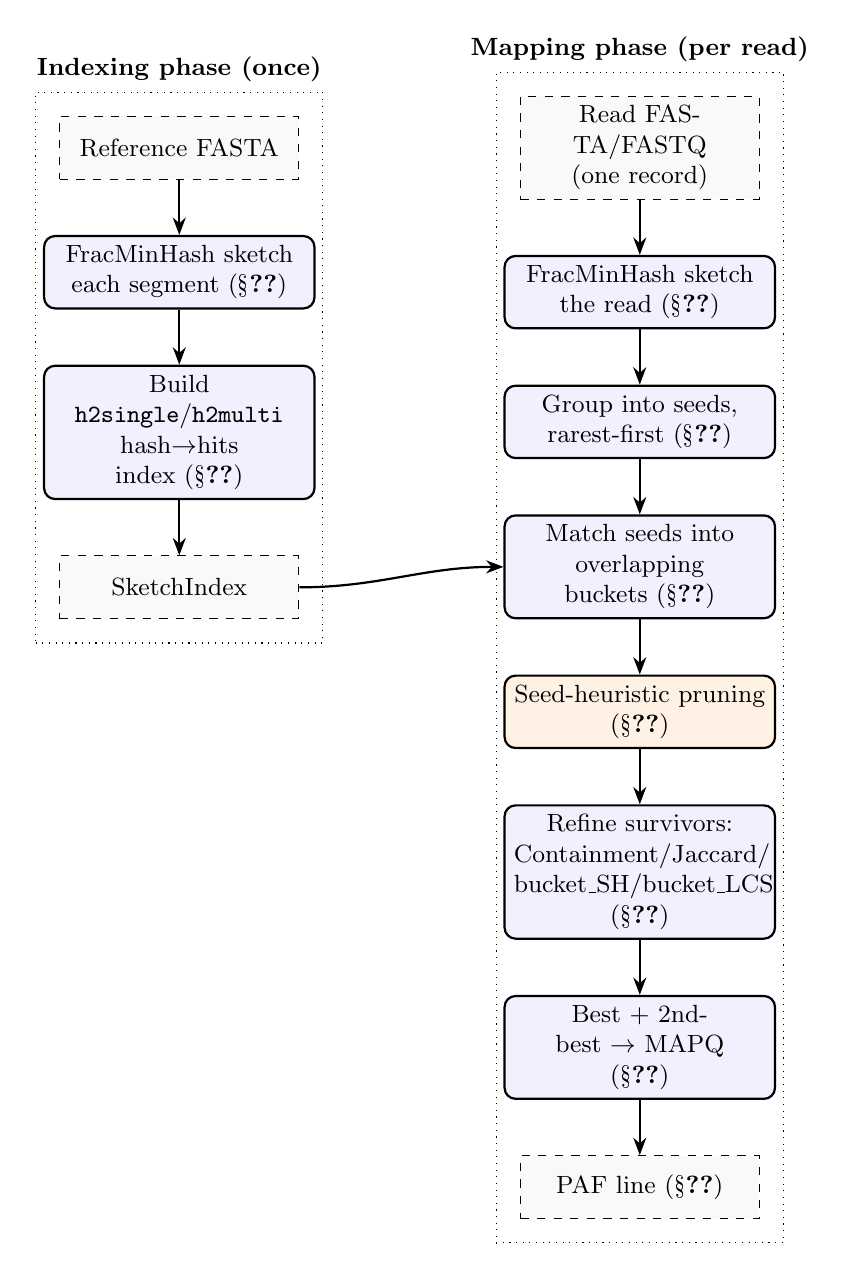
\begin{tikzpicture}[
    node distance=7mm and 12mm,
    every node/.style={font=\small},
    box/.style={draw, rounded corners, fill=blue!6, minimum height=9mm, text width=32mm, align=center, thick},
    dbox/.style={draw, rounded corners, fill=orange!10, minimum height=9mm, text width=32mm, align=center, thick},
    io/.style={draw, dashed, fill=gray!5, minimum height=8mm, text width=28mm, align=center},
    arr/.style={-{Stealth[length=2.2mm]}, thick}
  ]
  % Indexing phase (left column)
  \node[io] (reffa) {Reference FASTA};
  \node[box, below=of reffa] (sketchref) {FracMinHash sketch\\ each segment (\S\ref{ch:sketching})};
  \node[box, below=of sketchref] (index) {Build \code{h2single}/\code{h2multi}\\ hash$\to$hits index (\S\ref{ch:indexing})};
  \node[io, below=of index] (idx) {SketchIndex};

  \draw[arr] (reffa) -- (sketchref);
  \draw[arr] (sketchref) -- (index);
  \draw[arr] (index) -- (idx);

  % Mapping phase (right column), per read
  \node[io, right=28mm of reffa] (readfa) {Read FASTA/FASTQ\\ (one record)};
  \node[box, below=of readfa] (sketchread) {FracMinHash sketch\\ the read (\S\ref{ch:sketching})};
  \node[box, below=of sketchread] (seed) {Group into seeds,\\ rarest-first (\S\ref{ch:seeding})};
  \node[box, below=of seed] (bucket) {Match seeds into\\ overlapping buckets (\S\ref{ch:bucketing})};
  \node[dbox, below=of bucket] (prune) {Seed-heuristic pruning\\ (\S\ref{ch:pruning})};
  \node[box, below=of prune] (score) {Refine survivors:\\ Containment/Jaccard/\\bucket\_SH/bucket\_LCS (\S\ref{ch:scoring})};
  \node[box, below=of score] (mapq) {Best + 2nd-best $\to$ MAPQ\\ (\S\ref{ch:mapq})};
  \node[io, below=of mapq] (paf) {PAF line (\S\ref{ch:output})};

  \draw[arr] (readfa) -- (sketchread);
  \draw[arr] (sketchread) -- (seed);
  \draw[arr] (seed) -- (bucket);
  \draw[arr] (bucket) -- (prune);
  \draw[arr] (prune) -- (score);
  \draw[arr] (score) -- (mapq);
  \draw[arr] (mapq) -- (paf);

  \draw[arr] (idx.east) to[out=0,in=180] (bucket.west);
  \node at ($(idx)!0.5!(bucket)+(0,0)$) {};

  \node[draw, dotted, fit=(reffa)(idx), inner sep=3mm, label={[font=\bfseries\small]above:Indexing phase (once)}] (fitL) {};
  \node[draw, dotted, fit=(readfa)(paf), inner sep=3mm, label={[font=\bfseries\small]above:Mapping phase (per read)}] (fitR) {};
\end{tikzpicture}
\caption{shmap's two-phase pipeline. The indexing phase runs once; the mapping phase repeats for
every read in the query file, consulting the already-built index.}
\label{fig:pipeline}
\end{figure}

\section{Configuration axes: the three compile-time flags}
\label{sec:config-axes}

The reference C++ implementation parameterizes its core mapper class as a template,
\code{SHMapper<no\_bucket\_pruning, one\_sweep, abs\_pos>}, over three independent booleans. In
the original source these are \emph{compile-time} template parameters (so that the compiler can
specialize/inline branch-free code for whichever combination is selected at build time), but they
are semantically just three independent feature toggles, exposed at the CLI as \code{-P}, \code{-B},
\code{-F} respectively:

\begin{center}
\begin{tabular}{@{}lp{9.5cm}@{}}
\toprule
\textbf{Flag / parameter} & \textbf{Effect} \\
\midrule
\code{no\_bucket\_pruning} (\code{-P}) &
  When true, \emph{disables} the seed-heuristic pruning of \S\ref{sec:seed-heuristic-theory}
  entirely: every candidate bucket is fully scored. Correct but much slower; useful as a
  ground-truth oracle to verify pruning never discards a bucket it shouldn't. \\
\code{one\_sweep} (\code{-B}) &
  Intended (per its own \texttt{-B} help text, ``disregards seed heuristic and runs one sweep on
  all matches'') to skip the incremental per-bucket seed budget entirely and consider every seed
  at once. \emph{Chapter~\ref{ch:defects} documents that in the reference source this flag is
  fully dead: parsed, templated, and printed, but never once branched on inside the mapper.} \\
\code{abs\_pos} (\code{-F}) &
  Selects the coordinate space used for bucket indexing and window-size comparisons: \emph{sketch
  index} (position within the array of sketch $k$-mers, i.e. ``the $i$-th kept $k$-mer'') when
  false (default), or \emph{absolute nucleotide position} when true. This changes bucket boundary
  arithmetic throughout Chapters~\ref{ch:bucketing}--\ref{ch:scoring} (every place that reads
  \emph{``in sketch-index units, or nucleotide units if \code{abs\_pos}''}). \\
\bottomrule
\end{tabular}
\end{center}

\begin{notebox}
A from-scratch implementation does not need compile-time specialization to get shmap's
performance characteristics: these three booleans can equally well be ordinary runtime
parameters threaded through the mapping functions (this is exactly what the accompanying Rust
re-implementation does, using const generics only to keep the option of zero-cost specialization
available, not because runtime dispatch is fundamentally required). What \emph{is} essential to
preserve is that each one is read consistently by \emph{every} function that needs it --- the
original source's own bug catalogue (Chapter~\ref{ch:defects}) includes at least one flag that
looks load-bearing but silently isn't.
\end{notebox}

\section{The metric axis}
\label{sec:metric-axis}

Orthogonal to the three structural flags above, a fourth, purely-scoring-level axis selects
\emph{how} a surviving bucket's similarity score is computed (CLI flag \code{-m}, four values):
\code{Containment}, \code{Jaccard}, \code{bucket\_SH}, \code{bucket\_LCS}. These map directly onto
the theory of \S\ref{sec:fracminhash-theory} (containment/Jaccard) and \S\ref{sec:lis-theory}
(LCS); \code{bucket\_SH} is a degenerate/cheap option that reuses the seed-heuristic bound itself
as the final score (no refinement sweep at all). Full formulas are in
\S\ref{sec:metric-variants}.

\section{Data-flow summary: what crosses each module boundary}

\begin{center}
\begin{tabular}{@{}p{3.1cm}p{4.6cm}p{6cm}@{}}
\toprule
\textbf{Stage} & \textbf{Input} & \textbf{Output} \\
\midrule
Sketch reference & raw nucleotide bytes per segment & \code{Vec<Kmer>} per segment (position,
  hash, strand) \\
Build index & all segments' \code{Vec<Kmer>} & \code{hash} $\to$ \code{Hit} (unique) or
  \code{hash} $\to$ \code{Vec<Hit>} (repeated), each \code{Hit} carrying segment id + position \\
Sketch read & raw nucleotide bytes of the read & \code{Vec<Kmer>} \\
Seed & \code{Vec<Kmer>} of the read & \code{Vec<Seed>}: one entry per distinct hash, with
  occurrence count in the read and reference hit count, sorted rarest-reference-hit-first \\
Bucket / match seeds & \code{Vec<Seed>} (budget-limited prefix) + index & per-\code{(segment,
  bucket)} running \code{BucketContent} (seed count, match count, codirection, position range) \\
Prune & sorted buckets (most-matches-first) + remaining unconsumed seeds & surviving buckets only
  (most are discarded using $O(1)$ arithmetic per extension step) \\
Refine & one surviving bucket + the read's seed table & one \code{Mapping} (score, matched
  interval, strand, intersection count) \\
Best/second-best & every refined \code{Mapping} & the two highest, non-overlapping,
  \code{Mapping}s \\
MAPQ & best two scores + same-strand-seed counts & integer MAPQ in $\{0,5,60\}$ (shmap's concrete
  range; see Chapter~\ref{ch:mapq}) \\
Output & final \code{Mapping} (+ globally accumulated counters) & one PAF text line with custom
  tags \\
\bottomrule
\end{tabular}
\end{center}

\section{Complexity at a glance}

Let $n = |T|$ (total reference length), $m$ = a read's sketch size ($\approx r\cdot|P|$), and $S
\le m$ the seed budget actually consumed for that read (\S\ref{sec:seed-budget}). Indexing is
$O(n)$ time (one rolling-hash pass) and $O(rn)$ space (the kept fraction of $k$-mers). Per read:
seeding/sorting is $O(m\log m)$; seed matching against the index is $O(S \cdot \bar d)$ where
$\bar d$ is the average number of reference hits per consumed seed (bounded above by \code{-M},
the max-matches-per-kmer cap, \S\ref{sec:max-matches}); bucket pruning is, in the typical case
where most buckets are eliminated in $O(1)$ extensions, sublinear in the number of buckets touched;
and refinement of each surviving bucket costs $O(|\text{bucket}|)$ (a single linear sweep). Full
derivations are in Chapter~\ref{ch:complexity}.

\chapter{Core Data Types}
\label{ch:data-types}

This chapter specifies every value type used throughout the pipeline: its fields, the exact unit
and range of each field, and the invariants callers may assume. All positions use \textbf{signed}
32-bit integers throughout the reference implementation (a legacy of an earlier dependency on
\texttt{klib}, which does not support 64-bit positions) --- a from-scratch implementation
targeting references larger than $2^{31}$ bases should widen these, but should otherwise preserve
signedness, since several computations (bucket predecessor indices, sentinel $-1$ values)
rely on it.

\section{Scalar type aliases}

\begin{center}
\begin{tabularx}{\textwidth}{@{}llX@{}}
\toprule
\textbf{Alias} & \textbf{Underlying type} & \textbf{Meaning} \\
\midrule
\code{hash\_t} & \code{uint64\_t} & A $k$-mer's (canonical, XOR-combined) hash value. \\
\code{rpos\_t} & \code{int32\_t} & A position in the \emph{reference}: either a nucleotide offset
  or a sketch-array index, depending on context (see \code{abs\_pos}, \S\ref{sec:config-axes}). \\
\code{qpos\_t} & \code{int32\_t} & A position/count in the \emph{query} (read): nucleotide offset,
  sketch-array index, or a plain count (occurrence counts, seed budgets). \\
\code{segm\_t} & \code{int32\_t} & Index of a reference segment (0-based, in FASTA record order).
\\
\bottomrule
\end{tabularx}
\end{center}

\begin{notebox}
\code{rpos\_t} and \code{qpos\_t} are both plain 32-bit signed integers with no type-level
distinction in the original C++ (they are both \code{typedef}s for the same underlying type) ---
the split is purely for reader clarity about which ``space'' a value lives in. A from-scratch
implementation may use one integer type for both, but keeping the naming distinction in comments
is strongly recommended: several bugs found in the reference source (Chapter~\ref{ch:defects})
stem exactly from a value computed as a query-space quantity being fed into a
reference-space-typed slot, or vice versa.
\end{notebox}

\section{\code{Kmer}}
\label{sec:type-kmer}

A single sketched $k$-mer: its position, hash, and strand.

\begin{center}
\begin{tabularx}{\textwidth}{@{}llX@{}}
\toprule
\textbf{Field} & \textbf{Type} & \textbf{Meaning} \\
\midrule
\code{r} & \code{rpos\_t} & \textbf{Zero-based index of the $k$-mer's last (rightmost) nucleotide}
  in its source sequence. \emph{Not} the exclusive right boundary of the half-open window, despite
  what an earlier version of the source's own doc-comment claims --- verified precisely in
  \S\ref{sec:sketch-r-semantics}: for the $i$-th ($0$-based) $k$-mer of a sequence, $r = i+k-1$. \\
\code{h} & \code{hash\_t} & Canonical hash (XOR of forward and reverse-complement rolling hashes;
  \S\ref{sec:fracminhash-hash}). \\
\code{strand} & \code{bool} & \code{false} = forward strand ``won'' the hash comparison, \code{true}
  = reverse-complement did. See \S\ref{sec:fracminhash-hash} for exactly how this is decided. \\
\bottomrule
\end{tabularx}
\end{center}

Equality on \code{Kmer} (where defined at all) compares \emph{only} \code{h}; no code path in the
reference implementation actually calls it, however (confirmed by exhaustive cross-reference
during the Rust port) --- every equality check in the real algorithm compares \code{.h} fields
directly.

\section{\code{Hit}}
\label{sec:type-hit}

A \code{Kmer}'s occurrence \emph{in the reference}, with its reference-relative metadata attached.

\begin{center}
\begin{tabularx}{\textwidth}{@{}llX@{}}
\toprule
\textbf{Field} & \textbf{Type} & \textbf{Meaning} \\
\midrule
\code{r} & \code{rpos\_t} & Copied from the source \code{Kmer.r} (absolute nucleotide position
  of the hit's last base within its segment). \\
\code{tpos} & \code{rpos\_t} & Index of this hit \emph{within the segment's own sketch array}
  (i.e., ``this is the \code{tpos}-th kept $k$-mer of this reference segment''). \\
\code{strand} & \code{bool} & Copied from the source \code{Kmer.strand}. \\
\code{segm\_id} & \code{segm\_t} & Which reference segment this hit belongs to. \\
\bottomrule
\end{tabularx}
\end{center}

Constructed as \code{Hit(kmer, tpos, segm\_id)} --- \code{r} and \code{strand} are always copied
straight from the source \code{Kmer}; only \code{tpos} and \code{segm\_id} are supplied
independently.

\section{\code{Seed}}
\label{sec:type-seed}

One \emph{distinct} $k$-mer hash from a read's sketch, with everything the mapper needs to know
about how it behaves both in the read and in the reference.

\begin{center}
\begin{tabularx}{\textwidth}{@{}llX@{}}
\toprule
\textbf{Field} & \textbf{Type} & \textbf{Meaning} \\
\midrule
\code{kmer} & \code{Kmer} & One representative occurrence of this hash in the read (position
  is that of the \emph{first}, in sort order, occurrence --- see \S\ref{sec:seeding-grouping}). \\
\code{hits\_in\_t} & \code{rpos\_t} & Total number of times this hash occurs \emph{anywhere in the
  whole reference} (looked up via \code{SketchIndex::count}, \S\ref{sec:index-count}). Zero if
  the hash never occurs in the reference at all. \\
\code{occs\_in\_p} & \code{qpos\_t} & Number of times this hash occurs \emph{in the read itself}
  (i.e., the multiplicity of a repeated $k$-mer within one read). \\
\code{seed\_num} & \code{qpos\_t} & 0-based rank of this seed among all distinct seeds of the read,
  \emph{after} sorting rarest-reference-hit-first (\S\ref{sec:seeding-sort}) --- i.e., the order
  seeds are actually consumed in. \\
\code{pmatches} & \code{Vec<qpos\_t>} & \emph{Every} position in the read where this hash occurs,
  \textbf{sorted in decreasing order} (a direct consequence of the grouping sort's tie-break, \S
  \ref{sec:seeding-grouping}). Used only by the \code{bucket\_LCS} metric
  (\S\ref{sec:lcs-implementation}). \\
\bottomrule
\end{tabularx}
\end{center}

\section{\code{Match}}
\label{sec:type-match}

A pairing of one \code{Seed} (from the read) with one \code{Hit} (in the reference) that share a
hash.

\begin{center}
\begin{tabularx}{\textwidth}{@{}llX@{}}
\toprule
\textbf{Field} & \textbf{Type} & \textbf{Meaning} \\
\midrule
\code{seed} & \code{Seed} (by value in C++; by reference in the Rust port, see below) & The
  matched read-side seed. \\
\code{hit} & \code{Hit} & The matched reference-side hit. \\
\bottomrule
\end{tabularx}
\end{center}

\code{Match} additionally exposes \code{codirection()}, returning $+1$ if
\code{seed.kmer.strand == hit.strand} (the read and reference agree on strand at this $k$-mer) and
$-1$ otherwise; summing this over a candidate's matches is how strand (forward vs.\ reverse
complement) is inferred for the final PAF strand column.

\begin{notebox}
\textbf{Ownership matters here.} The C++ \code{Match} \emph{copies} the entire matched
\code{Seed} --- including its heap-allocated \code{pmatches} vector --- into itself, and
\code{Match} objects are constructed in the thousands per read (once per (seed, hit) pair
scanned during bucket collection and both refinement sweeps). This is a real, measurable cost in
the reference binary. The Rust re-implementation instead gives \code{Match} a borrow,
\code{seed: \&'p Seed}, tied to the lifetime of the read-scoped seed table it is built from ---
every \code{Vec<Match>} in the algorithm is constructed, consumed, and dropped within the
processing of a single read, so this lifetime is trivially satisfiable and eliminates the
per-match deep copy entirely. A future from-scratch implementation in a garbage-collected
language should simply share/reference the \code{Seed}, not clone it, for the same reason.
\end{notebox}

\section{\code{BucketLoc}}
\label{sec:type-bucketloc}

The coordinate of one bucket: which segment, and which half-length slot.

\begin{center}
\begin{tabularx}{\textwidth}{@{}llX@{}}
\toprule
\textbf{Field} & \textbf{Type} & \textbf{Meaning} \\
\midrule
\code{segm\_id} & \code{segm\_t} & Reference segment index. \\
\code{b} & \code{rpos\_t} & Bucket slot index; slot $b$ spans reference positions
  $[b\cdot\ell, (b{+}2)\cdot\ell)$ where $\ell$ is the current read's bucket half-length
  (\S\ref{sec:bucket-geometry}). \\
\bottomrule
\end{tabularx}
\end{center}

The default/sentinel value is $(-1,-1)$, used to mean ``no second-best bucket found yet'' in
output. This sentinel is part of the \emph{observable output format} (it is printed literally as
\code{(-1,-1)} in the \code{b2:s:} PAF tag when a read has no second-best mapping), so a
from-scratch implementation that wants byte-compatible output should preserve it as a real
sentinel value rather than, say, an optional/nullable type whose absence is rendered differently.

\section{\code{BucketContent}}
\label{sec:type-bucketcontent}

The running accumulator attached to each bucket as seeds are matched into it.

\begin{center}
\begin{tabularx}{\textwidth}{@{}lllX@{}}
\toprule
\textbf{Field} & \textbf{Type} & \textbf{Default} & \textbf{Meaning} \\
\midrule
\code{i} & \code{int} & $-1$ & Index of the next \emph{seed} (into the read's sorted seed list) to
  extend this bucket with, during incremental pruning (\S\ref{sec:seed-heuristic-pass}). \\
\code{seeds} & \code{qpos\_t} & $0$ & Seed \emph{occurrences} attributed to this bucket so far
  (\S\ref{sec:seed-heuristic-theory}). \\
\code{matches} & \code{qpos\_t} & $0$ & Of those, how many actually landed a hit in this bucket. \\
\code{codirection} & \code{int} & $0$ & Running sum of $\pm1$ per matched hit
  (\S\ref{sec:type-match}); sign indicates the dominant strand. \\
\code{r\_min}, \code{r\_max} & \code{rpos\_t} & $+\infty$, $-1$ & Smallest/largest nucleotide
  position (\code{Hit.r}) seen among this bucket's matches so far --- used directly as the
  candidate's reported boundary by the \code{bucket\_SH} metric. \\
\bottomrule
\end{tabularx}
\end{center}

\code{BucketContent} supports an additive merge (\code{operator+=} in C++, an \code{AddAssign}
impl in Rust) that sums \code{matches}/\code{seeds}/\code{codirection} and takes the
componentwise min/max of the position range --- used whenever two partial accumulations of the
same bucket need combining (e.g.\ a hit contributing to both bucket $b$ and its overlapping
neighbor $b{-}1$, \S\ref{sec:bucket-geometry}).

\section{\code{RefSegment}}
\label{sec:type-refsegment}

One indexed reference sequence (e.g.\ one chromosome/contig).

\begin{center}
\begin{tabularx}{\textwidth}{@{}llX@{}}
\toprule
\textbf{Field} & \textbf{Type} & \textbf{Meaning} \\
\midrule
\code{kmers} & \code{Vec<Kmer>} & This segment's full FracMinHash sketch, in increasing position
  order. \\
\code{name} & \code{String} & FASTA record id (used as the PAF target-name column and for
  ground-truth segment lookup, \S\ref{sec:ground-truth}). \\
\code{sz} & \code{rpos\_t} & Segment length in nucleotides (PAF target-length column). \\
\code{id} & \code{segm\_t} & This segment's own index (redundant with its position in the
  segment array, kept for convenience). \\
\bottomrule
\end{tabularx}
\end{center}

\begin{notebox}
The C++ \code{RefSegment} additionally stores the segment's full raw nucleotide sequence
(\code{seq}), intended for a SAM/CIGAR alignment feature that is entirely commented out and
unreachable in the shipped tool. Retaining it roughly doubles index memory for zero functional
benefit; a from-scratch implementation targeting only the mapping (not alignment) functionality
described in this document should omit it.
\end{notebox}

\section{Hash-map type aliases}

Four hash-map shapes recur throughout the algorithm; a from-scratch implementation may use any
hash map with average $O(1)$ get/insert (the reference C++ uses two different fast open-addressing
hash map libraries; the choice is a pure performance detail with no semantic effect):

\begin{center}
\begin{tabularx}{\textwidth}{@{}llX@{}}
\toprule
\textbf{Alias} & \textbf{Shape} & \textbf{Populated in / used by} \\
\midrule
\code{h2single} & \code{hash\_t} $\to$ \code{Hit} & Reference index, $k$-mers with exactly one
  occurrence (\S\ref{ch:indexing}). \\
\code{h2multi} & \code{hash\_t} $\to$ \code{Vec<Hit>} & Reference index, $k$-mers with $\ge 2$
  occurrences, each list sorted by \code{(segm\_id, r)} for binary search
  (\S\ref{sec:index-sort}). \\
\code{h2seed\_t} & \code{hash\_t} $\to$ \code{Seed} & Per-read seed lookup table, built once per
  read from its unique seeds (\S\ref{sec:seeding-grouping}). \\
\code{h2cnt} & \code{hash\_t} $\to$ \code{qpos\_t} & Per-read ``remaining occurrence budget''
  table (\code{diff\_hist}), decremented/incremented as a sliding window consumes/releases matches
  of a given hash during refinement (\S\ref{sec:scoring-sliding-window}); values may legitimately
  go negative transiently (see that section for why). \\
\bottomrule
\end{tabularx}
\end{center}

\section{\code{Mapping} and its stats sub-structures}
\label{sec:type-mapping}

A \code{Mapping} is the algorithm's single ``current best candidate'' record: it behaves like a
running maximum, only ever overwritten by \code{update(...)} when a strictly higher score is
found (initial score is the sentinel $-1.0$, guaranteed to lose to any real, non-negative
similarity score). It bundles three logical groups of fields:

\begin{center}
\begin{tabularx}{\textwidth}{@{}llX@{}}
\toprule
\textbf{Group} & \textbf{Represents} & \textbf{Key fields} \\
\midrule
\code{MappingPaf} & The 12 mandatory PAF columns (\S\ref{ch:output}) & \code{p\_start,p\_end,
  strand,segm\_name,segm\_sz,segm\_id,t\_l,t\_r,mapq,query\_id,p\_sz} \\
\code{LocalMappingStats} & Per-read/per-candidate diagnostics, always populated & \code{s\_sz}
  (matched reference span), \code{intersection}, \code{j}/\code{j2} (best/2nd-best score),
  \code{sh} (seed-heuristic value at acceptance), \code{bucket}/\code{bucket2} \\
\code{GlobalMappingStats} & Run-wide diagnostics, populated once per read only if a mapping was
  found & \code{seeds}, \code{total\_matches}, \code{seeded\_buckets}, \code{final\_buckets},
  \code{match\_inefficiency} \\
\bottomrule
\end{tabularx}
\end{center}

Full field-by-field definitions, exact default/sentinel values, and the precise PAF/tag text
each one is rendered as are given together with the output format in Chapter~\ref{ch:output},
since their only purpose is serialization; the \emph{algorithmic} methods that live on
\code{Mapping} (\code{update}, \code{set\_second\_best}, \code{calc\_mapq},
\code{overlap}) are specified where they are actually invoked: \code{update} in
Chapter~\ref{ch:scoring}, \code{set\_second\_best}/\code{overlap} in
Chapter~\ref{ch:end-to-end}, and \code{calc\_mapq} in Chapter~\ref{ch:mapq}.

\begin{notebox}
Two of \code{Mapping}'s stats fields deserve an early flag because they affect how a
from-scratch implementer should read every later chapter's arithmetic: \code{intersection2}
(second-best match count) and \code{bucket2} default to the sentinel values $-1$ and $(-1,-1)$
respectively, and \emph{stay there} for any read with no viable second-best candidate --- this is
a normal, expected, frequently-occurring output state (a uniquely-mapping read), not an error
state, and downstream formulas (notably \code{sigmas\_diff} and \code{calc\_mapq} in
Chapter~\ref{ch:mapq}) are specifically written to treat the sentinel $-1$ as ``$0$'' rather than
its literal value.
\end{notebox}

\chapter{FracMinHash Sketching}
\label{ch:sketching}

This chapter specifies \code{FracMinHash::sketch}, the single most bit-sensitive routine in the
whole system: every downstream index, seed, and score depends on hashes being computed exactly
this way, since reference and read sketches must use an \emph{identical} hash function to be
comparable at all.

\section{Inputs and outputs}

\begin{center}
\begin{tabular}{@{}p{2.6cm}p{4.5cm}p{7cm}@{}}
\toprule
& \textbf{Type} & \textbf{Meaning} \\
\midrule
\textit{Input} \code{s} & raw ASCII nucleotide bytes (upper- or lower-case \code{A/C/G/T};
  anything else, see \S\ref{sec:sketch-nonacgt}) & The sequence to sketch: one reference segment,
  or one read. \\
\textit{Config} \code{k} & positive integer & $k$-mer length (CLI \code{-k}, default 15). \\
\textit{Config} \code{h\_frac} & $r \in (0,1]$ & Keep-fraction of the hash space (CLI \code{-r},
  default 0.05). \\
\textit{Output} & \code{Vec<Kmer>} & Every $k$-mer of \code{s} whose canonical hash clears the
  threshold, in increasing position order, each tagged with its hash and winning strand
  (\S\ref{sec:type-kmer}). Empty if $|s| < k$. \\
\bottomrule
\end{tabular}
\end{center}

\section{Lookup tables: per-nucleotide hash contributions}
\label{sec:sketch-lut}

The rolling hash is built from two 256-entry lookup tables, \code{LUT\_fw} and \code{LUT\_rc},
indexed by raw ASCII byte value, giving each of the four nucleotides (in both upper and lower
case) a fixed 64-bit contribution:

\begin{center}
\begin{tabularx}{\textwidth}{@{}llX@{}}
\toprule
Base & \code{LUT\_fw} contribution (hex) & \code{LUT\_rc} contribution \\
\midrule
A/a & \code{0x3c8bfbb395c60474} & = \code{LUT\_fw['T']} \\
C/c & \code{0x3193c18562a02b4c} & = \code{LUT\_fw['G']} \\
G/g & \code{0x20323ed082572324} & = \code{LUT\_fw['C']} \\
T/t & \code{0x295549f54be24456} & = \code{LUT\_fw['A']} \\
\bottomrule
\end{tabularx}
\end{center}

That is, a base's reverse-complement contribution is defined as its \emph{complementary} base's
forward contribution --- exactly encoding the biological complement rule (A$\leftrightarrow$T,
C$\leftrightarrow$G) at the hash-contribution level, so that no explicit ``complement a
character'' step is ever needed; complementation falls out of table lookup alone. All other byte
values (N, ambiguity codes, whitespace, etc.) have \emph{no defined contribution} in the reference
source.

\begin{bugbox}
The reference C++ declares \code{LUT\_fw}/\code{LUT\_rc} as plain fixed-size arrays and
initializes only the 8 entries above; the remaining 248 entries are \textbf{uninitialized stack
memory} at the time \code{sketch()} first reads them. For any input byte other than
\texttt{ACGTacgt} (most commonly \texttt{N}), the hash computation silently incorporates garbage.
This is undefined behavior, not merely ``an unspecified but fixed value'' --- the actual bits
read depend on whatever happened to be on the stack. \textbf{Recommended fix for a from-scratch
implementation:} zero-initialize both tables before filling in the 8 real entries, so that any
non-ACGT byte deterministically contributes a hash of $0$. This changes no behavior for any
ACGT-only input (which is the overwhelming majority of real sequence data) and removes the UB.
\end{bugbox}

\section{The position semantics of \code{Kmer.r}}
\label{sec:sketch-r-semantics}

Before giving the recurrence, it is worth nailing down precisely what value ends up in a produced
\code{Kmer}'s \code{r} field, since it is easy to get this off by one and it is exercised by the
reference test suite. For the ($0$-based) $i$-th $k$-mer of a sequence (spanning nucleotide
positions $[i, i{+}k)$):
\[
  \texttt{Kmer.r} = i + k - 1
\]
i.e., \textbf{the index of the $k$-mer's last nucleotide}, not the exclusive upper bound of its
span (despite a doc-comment in the reference source claiming the latter). This is verified by the
reference test suite itself: for $k=4$ and a 5-character sequence, the two produced $k$-mers (at
$i=0,1$) have \code{r} $=3,4$ respectively, matching $i+k-1$.

\section{The rolling-hash recurrence}
\label{sec:fracminhash-hash}

Let $s$ be the input, $k$ the $k$-mer length, and define, for a byte $c$, $\mathrm{fw}(c) =
\text{\code{LUT\_fw}}[c]$ and $\mathrm{rc}(c) = \text{\code{LUT\_rc}}[c]$. The threshold is
\[
  H_{\mathrm{thr}} = \begin{cases} \lfloor r \cdot (2^{64}-1) \rfloor & r < 1 \\ 2^{64}-1 & r = 1
  \end{cases}
\]
computed once via a floating-point multiply-then-truncate (this is the one place floating-point
rounding can matter at all --- for $r=1$ it is special-cased to the exact maximum, avoiding any
rounding).

\paragraph{Initialization (first window, $i=0$).} Seed $h_{fw}=h_{rc}=0$, then fold in each of the
first $k$ bases with a position-dependent rotation:
\[
  h_{fw} \mathrel{\oplus}= \mathrm{rotl}\bigl(\mathrm{fw}(s[j]),\; k-j-1\bigr), \qquad
  h_{rc} \mathrel{\oplus}= \mathrm{rotl}\bigl(\mathrm{rc}(s[j]),\; j\bigr)
  \qquad\text{for } j = 0,\dots,k-1.
\]
(\(\mathrm{rotl}(x,n)\) / \(\mathrm{rotr}(x,n)\) denote 64-bit bitwise left/right rotation.) Note
the two hashes rotate in \emph{opposite} directions and by \emph{mirrored} amounts ($k{-}j{-}1$
vs.\ $j$) --- this is precisely what makes $h_{rc}$ equal to the forward hash of the
reverse-complement string: reversing the string reverses which position gets which rotation
amount, and complementing each base is handled already by using \code{LUT\_rc} instead of
\code{LUT\_fw}.

\paragraph{Emitting a $k$-mer.} At every window position (including the very first, before any
roll), combine the two sides and test the threshold:
\[
  h = h_{fw} \oplus h_{rc}, \qquad \text{keep iff } h \le H_{\mathrm{thr}}.
\]
If kept, its strand bit is $\;\texttt{strand} = (h_{fw} > h_{rc})\;$ --- i.e., whichever side is
numerically larger is deemed to have ``won'' and determines orientation. (This is an arbitrary
but self-consistent convention: swap the comparison and every strand bit flips consistently, with
no effect on any similarity computation, since those only ever compare two \code{Kmer}s'/\code{
Hit}s' strand bits to each other, never to an absolute notion of ``forward''.)

\paragraph{Rolling to the next window ($i \to i+1$, incoming base $s[i{+}k]$, outgoing base
$s[i]$).}
\[
  h_{fw} \leftarrow \mathrm{rotl}(h_{fw}, 1) \;\oplus\; \mathrm{rotl}(\mathrm{fw}(s[i]), k)
  \;\oplus\; \mathrm{fw}(s[i{+}k])
\]
\[
  h_{rc} \leftarrow \mathrm{rotr}(h_{rc}, 1) \;\oplus\; \mathrm{rotr}(\mathrm{rc}(s[i]), 1)
  \;\oplus\; \mathrm{rotl}(\mathrm{rc}(s[i{+}k]), k-1)
\]
Each update: (1) rotates the whole accumulated hash by one position in the direction that side
rolls, (2) removes the outgoing base's contribution (itself rotated to the position it now needs
to cancel from), (3) adds the incoming base's contribution at its new position. This is the
standard structure of an XOR/rotate rolling hash: rotation distributes each base's contribution
across all 64 bits over the $k$-window it participates in, and since $\mathrm{rotl}$/$\mathrm{rotr}$
are self-inverse under repeated application by the same total, the outgoing base's contribution
cancels \emph{exactly} (XOR with itself) once it has rolled all the way through.

\begin{algobox}{title={\code{sketch}(s, k, h\_frac)}}
\begin{verbatim}
if len(s) < k: return []
H_thr := (h_frac < 1) ? floor(h_frac * (2^64 - 1)) : 2^64 - 1
h_fw, h_rc := 0, 0
for j in 0..k-1:
    h_fw ^= rotl(LUT_fw[s[j]], k-j-1)
    h_rc ^= rotl(LUT_rc[s[j]], j)
r := k - 1              # position of the k-mer's last base, 0-based
result := []
loop:
    h := h_rc ^ h_fw
    if h <= H_thr:
        strand := (h_fw > h_rc)
        result.append(Kmer{ r: r, h: h, strand: strand })
    if r + 1 >= len(s): break
    out_c, in_c := s[r + 1 - k], s[r + 1]
    h_fw := rotl(h_fw, 1) ^ rotl(LUT_fw[out_c], k) ^ LUT_fw[in_c]
    h_rc := rotr(h_rc, 1) ^ rotr(LUT_rc[out_c], 1) ^ rotl(LUT_rc[in_c], k-1)
    r := r + 1
return result
\end{verbatim}
\end{algobox}

\begin{notebox}
The loop above is written with the loop variable \code{r} directly holding the emitted
\code{Kmer.r} value at every iteration (equivalent to, but clearer than, the reference source's
own \code{for(r=0;...) ... push(Kmer(r-1,...))} formulation, which tracks ``one past'' internally
and subtracts 1 only at emission time). Both are exactly equivalent; verify against
\S\ref{sec:sketch-r-semantics} if re-deriving independently.
\end{notebox}

\section{Reference C++ implementation}

\begin{lstlisting}[style=cppstyle,caption={\code{FracMinHash::sketch}, \texttt{src/sketch.h} (verbatim)}]
const sketch_t sketch(const std::string& s) const {
    sketch_t kmers;
    kmers.reserve((rpos_t)(1.1 * (double)s.size() * hFrac));
    if (rpos_t(s.size()) < k) return kmers;

    hash_t h_fw = 0, h_rc = 0;
    hash_t hThres = hFrac < 1.0
        ? hash_t(hFrac * double(std::numeric_limits<hash_t>::max()))
        : std::numeric_limits<hash_t>::max();
    rpos_t r;

    for (r=0; r<k; r++) {
        h_fw ^= std::rotl(LUT_fw[ size_t(s[r]) ], k-r-1);
        h_rc ^= std::rotl(LUT_rc[ size_t(s[r]) ], r);
    }

    while(true) {
        auto h = h_rc ^ h_fw;
        if (h <= hThres) {
            const bool strand = h_fw > h_rc;
            kmers.push_back(Kmer(r-1, h, strand));
        }
        if (r >= rpos_t(s.size())) break;
        h_fw = std::rotl(h_fw, 1) ^ std::rotl(LUT_fw[ size_t(s[r-k]) ], k) ^ LUT_fw[ size_t(s[r]) ];
        h_rc = std::rotr(h_rc, 1) ^ std::rotr(LUT_rc[ size_t(s[r-k]) ], 1)
             ^ std::rotl(LUT_rc[ size_t(s[r]) ], k-1);
        ++r;
    }
    return kmers;
}
\end{lstlisting}

\section{Rust re-implementation}

\begin{lstlisting}[style=rststyle,caption={\code{FracMinHash::sketch}, Rust port (\texttt{src/sketch.rs})}]
pub fn sketch(&self, s: &[u8], counters: &mut Counters) -> SketchT {
    let k = self.k;
    let mut kmers: SketchT =
        Vec::with_capacity((1.1 * s.len() as f64 * self.h_frac).max(0.0) as usize);
    if (s.len() as RPos) < k { return kmers; }

    let h_thres: Hash = if self.h_frac < 1.0 {
        (self.h_frac * u64::MAX as f64) as u64
    } else { u64::MAX };

    let mut h_fw: Hash = 0;
    let mut h_rc: Hash = 0;
    let mut r: RPos = 0;
    while r < k {
        let c = s[r as usize] as usize;
        h_fw ^= self.lut_fw[c].rotate_left((k - r - 1) as u32);
        h_rc ^= self.lut_rc[c].rotate_left(r as u32);
        r += 1;
    }

    loop {
        let h = h_rc ^ h_fw;
        if h <= h_thres {
            let strand = h_fw > h_rc;
            kmers.push(Kmer::new(r - 1, h, strand));
        }
        if r >= s.len() as RPos { break; }
        let out_c = s[(r - k) as usize] as usize;
        let in_c = s[r as usize] as usize;
        h_fw = h_fw.rotate_left(1) ^ self.lut_fw[out_c].rotate_left(k as u32) ^ self.lut_fw[in_c];
        h_rc = h_rc.rotate_right(1)
            ^ self.lut_rc[out_c].rotate_right(1)
            ^ self.lut_rc[in_c].rotate_left((k - 1) as u32);
        r += 1;
    }
    kmers
}
\end{lstlisting}

Note the Rust version zero-initializes both LUTs before filling the 8 real entries (the fix from
the bug box above); everything else is a direct, bit-for-bit translation --- \code{rotate\_left}/
\code{rotate\_right} on a \code{u64} are exactly \code{std::rotl}/\code{std::rotr} on
\code{uint64\_t}, including the fact that both are defined for \emph{any} shift amount (taken mod
64), so no extra bounds-masking is needed even though $k$ can exceed typical small shift-amount
assumptions.

\section{Non-ACGT input}
\label{sec:sketch-nonacgt}

Real sequencing data occasionally contains \texttt{N} (unknown base) or, rarely, IUPAC ambiguity
codes. As established above, the reference implementation's behavior on these is undefined; the
recommended, safe, deterministic choice --- adopted by the Rust port --- is that such a byte
contributes a hash of exactly $0$ on both the forward and reverse-complement side. This is a
reasonable default because it is simple, deterministic, and does not privilege any particular
real base; a from-scratch implementation is free to choose a different deterministic convention
(e.g.\ skip $k$-mers containing any non-ACGT byte entirely, which several other tools do) as long
as it is applied \emph{identically} when sketching the reference and the reads, since any
asymmetry there would silently break matching.

\section{Complexity}

Sketching a sequence of length $n$ takes $O(n)$ time (one $O(1)$-amortized rolling-hash step per
position, after an $O(k)$ initialization) and produces, in expectation, $O(rn)$ output $k$-mers,
using $O(rn)$ space for the output (input is streamed, not buffered beyond what the caller already
holds).

\section{Worked example}

For $k=4$, $r=1.0$ (keep everything) and input \texttt{"ACGGT"} (length 5, so 2 $k$-mers), the two
produced \code{Kmer}s have \code{r} $= 3, 4$ (matching $i+k-1$ for $i=0,1$). Feeding the
reverse complement of the same underlying sequence, \texttt{"ACCGT"}, produces the \emph{same
multiset of hashes} in reversed position order and with each \code{strand} bit flipped relative to
the original --- this symmetry (verified as an automated test in both the C++ and Rust
implementations) is the single most important sanity check to run against any from-scratch
reimplementation before trusting it: sketch a string and its reverse complement, reverse one
result, and confirm the hash sequences match exactly.

\chapter{Reference Indexing}
\label{ch:indexing}

The index (\code{SketchIndex}) is built exactly once per run, from the reference FASTA, before any
read is processed. Its job is to answer, in $O(1)$ average time, two questions for any $k$-mer
hash $h$: \emph{how many times does $h$ occur in the reference} (\S\ref{sec:index-count}), and
\emph{at which (segment, position) pairs} (used throughout bucketing/scoring).

\section{Data owned by the index}

\begin{center}
\begin{tabularx}{\textwidth}{@{}llX@{}}
\toprule
\textbf{Field} & \textbf{Type} & \textbf{Meaning} \\
\midrule
\code{segments} & \code{Vec<RefSegment>} & One entry per FASTA record, in file order
  (\S\ref{sec:type-refsegment}). \\
\code{h2single} & \code{hash\_t} $\to$ \code{Hit} & $k$-mers occurring \emph{exactly once} across
  the whole reference. \\
\code{h2multi} & \code{hash\_t} $\to$ \code{Vec<Hit>} & $k$-mers occurring \emph{two or more}
  times, each list sorted (\S\ref{sec:index-sort}). \\
\bottomrule
\end{tabularx}
\end{center}

Splitting single- vs.\ multi-occurrence $k$-mers into two separate maps (rather than one map to
always-a-list) is a memory/speed optimization: the overwhelming majority of $k$-mers in a
non-repetitive genome occur exactly once, so storing those as a bare \code{Hit} (no vector
indirection/allocation) rather than a one-element \code{Vec<Hit>} meaningfully reduces both memory
and pointer-chasing.

\section{Building the index: \code{build\_index}}

\begin{algobox}{title={\code{build\_index}(t\_file, k, h\_frac, max\_matches)}}
\begin{verbatim}
for (segm_name, seq) in read_fasta(t_file):
    sketch := FracMinHash.sketch(seq, k, h_frac)          # Chapter 5
    segm_id := len(segments)
    segments.append(RefSegment{ kmers: sketch, name: segm_name,
                                 sz: len(seq), id: segm_id })
    populate_h2pos(sketch, segm_id)                        # below

# migrate any hash that ended up in BOTH maps fully into h2multi
for (h, hits) in h2multi:
    if h in h2single:
        hits.append(h2single.remove(h))
    sort hits by (segm_id, r)                               # enables binary search later

if max_matches is set:
    erase_frequent_kmers(max_matches)                       # below
\end{verbatim}
\end{algobox}

\subsection{\code{populate\_h2pos}: routing each hit to the right map}
\label{sec:index-populate}

\begin{algobox}{title={\code{populate\_h2pos}(sketch, segm\_id)}}
\begin{verbatim}
for tpos, kmer in enumerate(sketch):
    hit := Hit(kmer, tpos, segm_id)
    if kmer.h not in h2single:
        h2single[kmer.h] := hit                 # first-ever occurrence: goes to h2single
    else:
        # second-or-later occurrence: goes to h2multi (h2single's own
        # earlier entry is migrated into h2multi at the *end* of indexing,
        # not immediately -- see build_index above)
        if max_matches is unset or len(h2multi[kmer.h]) < max_matches + 1:
            h2multi[kmer.h].append(hit)
\end{verbatim}
\end{algobox}

\begin{notebox}
Note the asymmetry this creates \emph{during} indexing (before the end-of-\code{build\_index}
migration step runs): a hash with exactly 2 occurrences temporarily has its \emph{first}
occurrence sitting in \code{h2single} and only its \emph{second} occurrence in \code{h2multi} ---
\code{h2multi[h]} would report length 1, not 2, if queried mid-build. This is why the migration
step (moving \code{h2single}'s entry into \code{h2multi} and \emph{erasing} it from
\code{h2single}) must run once, after all segments have been sketched, before the index is
considered complete and used for querying.
\end{notebox}

The \code{max\_matches + 1} cap during population (rather than exactly \code{max\_matches}) is
deliberate slack: it lets \code{erase\_frequent\_kmers} (below) later distinguish ``exactly at the
cap'' from ``over the cap'' after the single-entry migration adds one more; in practice, since
\code{erase\_frequent\_kmers} deletes any hash whose \emph{final} count exceeds \code{max\_matches}
outright, the effect is simply an upper bound on wasted work spent appending hits for a hash that
is going to be discarded anyway.

\subsection{Sorting multi-hit lists}
\label{sec:index-sort}

Each \code{h2multi} list is sorted by \code{(segm\_id, r)} lexicographically. Because $r$ (a
hit's nucleotide position) and $\mathit{tpos}$ (its index into the segment's own sketch array)
increase together within one segment (the sketch is built and stored in increasing position
order, \S\ref{sec:type-refsegment}), sorting by $r$ \emph{also} sorts by $\mathit{tpos}$
consistently --- so binary search by either coordinate space works correctly against the same
sorted list, which matters because bucket/window boundary checks are expressed in \emph{either}
space depending on the \code{abs\_pos} flag (\S\ref{sec:config-axes}).

\subsection{\code{erase\_frequent\_kmers}: capping pathologically repetitive $k$-mers}
\label{sec:max-matches}

CLI flag \code{-M} sets \code{max\_matches}, an optional hard cap on how many reference
occurrences a single $k$-mer hash is allowed to have before it is discarded from the index
entirely (treated thereafter as if it never occurred in the reference at all, i.e.\
\code{hits\_in\_t} $=0$ for it). This exists because extremely repetitive $k$-mers (satellite
repeats, low-complexity runs) contribute enormous numbers of hits that are almost never
informative for mapping but are expensive to iterate during seeding/bucketing --- capping them is
a standard technique shared with essentially every other $k$-mer-based mapper (minimap2's
\texttt{-f}, Winnowmap's repetitive-$k$-mer blacklist, etc.).

\begin{algobox}{title={\code{erase\_frequent\_kmers}(max\_matches)}}
\begin{verbatim}
for (h, hits) in h2multi:
    if len(hits) > max_matches:
        delete h2multi[h]
\end{verbatim}
\end{algobox}

Note this only prunes \code{h2multi} (by construction, \code{h2single} entries always have exactly
one occurrence, so they can never exceed any cap $\ge 1$).

\section{\code{count(h)}: reference occurrence count for a hash}
\label{sec:index-count}

\begin{algobox}{title={\code{count}(h)}}
\begin{verbatim}
if h in h2single: return 1
if h in h2multi:  return len(h2multi[h])
return 0
\end{verbatim}
\end{algobox}

This is the function seeding (Chapter~\ref{ch:seeding}) calls once per distinct read $k$-mer to
determine \code{hits\_in\_t} (\S\ref{sec:type-seed}) --- it is the quantity seeds are sorted by
(rarest first) and the input to the seed-heuristic bound's implicit assumption that
\code{hits\_in\_t}$=0$ seeds contribute nothing.

\section{Reference C++ implementation}

\begin{lstlisting}[style=cppstyle,caption={Core of \code{SketchIndex}, \texttt{src/index.h}}]
inline rpos_t count(hash_t h) const {
    if (auto it = h2single.find(h); it != h2single.end()) return 1;
    if (auto it = h2multi.find(h); it != h2multi.end()) return it->second.size();
    return 0;
}

void populate_h2pos(const sketch_t& sketch, segm_t segm_id) {
    for (size_t tpos = 0; tpos < sketch.size(); ++tpos) {
        const Kmer& kmer = sketch[tpos];
        const auto hit = Hit(kmer, tpos, segm_id);
        if (!h2single.contains(kmer.h))
            h2single[kmer.h] = hit;
        else if (H->params.max_matches == -1
                 || (rpos_t)h2multi[kmer.h].size() < H->params.max_matches + 1)
            h2multi[kmer.h].push_back(hit);
    }
}

void build_index(const std::string &tFile) {
    read_fasta_klib(tFile, [this](const string &segm_name, const string &T, float) {
        sketch_t t = H->sketcher.sketch(T);
        add_segment(segm_name, T, t);   // pushes RefSegment, calls populate_h2pos
    });

    for (auto &[h, hits] : h2multi) {
        if (h2single.contains(h)) {
            hits.push_back(h2single.at(h));
            h2single.erase(h);
        }
        sort(hits.begin(), hits.end(), [](const Hit &a, const Hit &b) {
            if (a.segm_id != b.segm_id) return a.segm_id < b.segm_id;
            return a.r < b.r;
        });
    }
    if (H->params.max_matches != -1) erase_frequent_kmers();
}
\end{lstlisting}

\section{Complexity and memory}

Indexing costs $O(n)$ time for sketching (Chapter~\ref{ch:sketching}) plus $O(rn \log d)$ for
sorting, where $rn$ is the total number of kept $k$-mers and $d$ is the maximum multiplicity of
any single hash (the sort is per-hash, so the $\log d$ factor applies independently to each
list, not globally). Memory is $O(rn)$: one map entry per distinct occurrence, plus $O(rn)$ for the
stored per-segment sketches themselves (each \code{RefSegment.kmers}).

\chapter{Seeding}
\label{ch:seeding}

Seeding turns a read's raw sketch (a flat list of $k$-mers, with repeats) into an ordered list of
\emph{seeds} --- one entry per distinct hash --- ready to be consumed budget-first against the
index. This chapter covers \code{unique\_elements\_with\_info} (grouping) and the derivation of
the seed budget $S$ used by the caller.

\section{Grouping: \code{unique\_elements\_with\_info}}
\label{sec:seeding-grouping}

\paragraph{Input.} \code{p}: the read's sketch, \code{Vec<Kmer>} (Chapter~\ref{ch:sketching}),
mutable (it is sorted in place). \emph{Implicit input:} the reference index, queried once per
distinct hash.

\paragraph{Output.} \code{Vec<Seed>} (\S\ref{sec:type-seed}), one per distinct hash value present
in \code{p}, \textbf{sorted ascending by \code{hits\_in\_t}} (rarest-in-reference first). Also
has the side effect of updating the \code{kmers\_notmatched} diagnostic counter
(\S\ref{sec:defect-notmatched} documents a bug in how the reference computes this specific
counter --- it does not affect any other output).

\begin{algobox}{title={\code{unique\_elements\_with\_info}(p)}}
\begin{verbatim}
# Step 1: group equal hashes together, and within a group, order by
# *decreasing* read position (this ordering becomes each seed's pmatches
# list, which the bucket_LCS metric consumes directly, see 10.4).
sort p by (h ascending, r descending)

# Step 2: walk the sorted list, closing out a group whenever the hash changes.
p_unique := []
strike := 0                 # occurrences seen in the current group so far
matches := []                # positions seen in the current group so far
for pos in 0 .. len(p)-1:
    strike += 1
    matches.append(p[pos].r)
    if pos == len(p)-1 or p[pos].h != p[pos+1].h:
        hits_in_t := index.count(p[pos].h)                # Section 6.4
        p_unique.append(Seed{
            kmer: p[pos], hits_in_t: hits_in_t,
            occs_in_p: strike, seed_num: len(p_unique),
            pmatches: copy(matches),
        })
        strike := 0
        matches := []

# Step 3: seeds are consumed rarest-reference-hit-first.
sort p_unique by hits_in_t ascending
return p_unique
\end{verbatim}
\end{algobox}

\paragraph{Why sort by \code{hits\_in\_t} ascending.} A $k$-mer that occurs rarely in the
reference is far more discriminative than a common one: matching it narrows the candidate set of
buckets dramatically, whereas matching a $k$-mer with thousands of reference occurrences adds
thousands of (mostly irrelevant) candidate hits for very little narrowing benefit. Consuming
seeds rarest-first under a fixed budget $S$ (\S\ref{sec:seed-budget}) maximizes the discriminative
value extracted from that budget.

\paragraph{Why sort the group by decreasing position.} \code{Seed.pmatches} ends up populated in
the same order the group was scanned, i.e.\ decreasing read position --- this specific order is
required by \code{lcs\_get\_lis} (\S\ref{sec:lcs-implementation}), which needs \code{pmatches} in
a defined order to reconstruct multiplicities correctly across repeated seeds when computing a
longest increasing subsequence.

\subsection{Reference C++ implementation}

\begin{lstlisting}[style=cppstyle,caption={\code{unique\_elements\_with\_info}, \texttt{src/shmap.h}}]
Seeds unique_elements_with_info(sketch_t& p) {
    sort(p.begin(), p.end(), [](const Kmer &a, const Kmer &b) {
        if (a.h != b.h) return a.h < b.h;
        return a.r > b.r;                 // reverse order of inclusion; needed for LCS
    });

    Seeds p_unique;
    qpos_t strike = 0;
    vector<qpos_t> matches;
    for (size_t ppos = 0; ppos < p.size(); ++ppos) {
        ++strike;
        matches.push_back(p[ppos].r);
        if (ppos == p.size()-1 || p[ppos].h != p[ppos+1].h) {
            rpos_t hits_in_t = tidx.count(p[ppos].h);
            p_unique.emplace_back(p[ppos], hits_in_t, strike, p_unique.size(), matches);
            strike = 0;
            matches.clear();
        }
    }

    sort(p_unique.begin(), p_unique.end(), [](const Seed &a, const Seed &b) {
        return a.hits_in_T < b.hits_in_T;
    });
    return p_unique;
}
\end{lstlisting}

\begin{bugbox}
\label{sec:defect-notmatched}
The reference C++ additionally maintains a \code{nonzero} counter meant to track how many
\emph{read positions} (counting multiplicity) belong to seeds that do have at least one reference
hit, so that the diagnostic \code{kmers\_notmatched} stat can report ``sketch size minus
matched positions''. The increment is written as \code{if (hits\_in\_t > 0) nonzero += strike;}
placed \emph{after} \code{strike} has already been reset to $0$ for the next group two lines
above it --- so it always adds $0$, and \code{kmers\_notmatched} always reports the entire sketch
size regardless of how many $k$-mers actually matched. This affects \emph{only} a cosmetic,
end-of-run diagnostic percentage; it has no effect on any mapping decision, score, or PAF field.
A from-scratch implementation should compute the increment \emph{before} resetting \code{strike}
(or reorder the two statements), which is the obviously-intended behavior.
\end{bugbox}

\section{The seed budget $S$}
\label{sec:seed-budget}

Not every seed is necessarily consumed --- seeding stops once a budget $S$ of seed
\emph{occurrences} (not distinct seeds; a repeated $k$-mer with \code{occs\_in\_p}$=3$ counts as
$3$ against the budget when consumed, all at once, \S\ref{sec:match-seeds}) has been spent. $S$ is
derived once per read from the acceptance threshold $\theta$ (CLI \code{-t}) and the
minimum-score-gap parameter (CLI \code{-d}, used here as a safety margin, not in its other role
computing the second-best threshold in Chapter~\ref{ch:end-to-end}):
\[
  \theta_2 = \theta - \mathit{min\_diff}, \qquad
  S = \left\lfloor (1-\theta_2)\cdot m \right\rfloor + 1
\]
where $m$ is the read's full sketch size. \textbf{Interpretation:} $S$ is exactly the smallest
seed-occurrence budget for which it is still \emph{possible}, in principle, for a bucket to reach
score $\theta_2$ even if literally every consumed seed occurrence that has a reference hit at all
ends up matching the same bucket: the seed-heuristic bound (\S\ref{sec:seed-heuristic-theory})
for a bucket that has consumed all $S$ seed occurrences and matched every one of them is exactly
$h_{\mathrm{seed}} = 1 - 0/m$, and the bound only starts to allow room for \emph{misses} once more
than $(1-\theta_2)m$ occurrences have been consumed --- so $S$ is the minimum budget that gives the
pruning bound any chance of staying above $\theta_2$ for a maximally-good bucket, with $+1$
guaranteeing at least one seed is always consumed even when $\theta_2 \to 1$.

\begin{notebox}
This is a heuristic sizing choice, not a hard correctness requirement in either direction: seeds
\emph{beyond} $S$ might still have found valuable matches (this is a real, accepted
recall/speed trade-off, and is exactly the knob CLI flag \code{-t} tunes indirectly through
$\theta_2$); a from-scratch implementation experimenting with alternative sizing should keep in
mind that $S$ only bounds how many seed \emph{occurrences} are matched against the index at all
--- it does not, by itself, bound the pruning behavior described in Chapter~\ref{ch:pruning},
which operates independently per bucket using whatever prefix of seeds \emph{has} been consumed
so far.
\end{notebox}

\section{\code{more\_seeds\_if\_cheap}: opportunistic budget extension (dead code)}

\begin{algobox}{title={\code{more\_seeds\_if\_cheap}(S, seeds)}}
\begin{verbatim}
original_S := S
while S < len(seeds) and seeds[S].hits_in_t <= 1:
    S += 1
return S
\end{verbatim}
\end{algobox}

This extends the budget past $S$ for free whenever the next seed(s) are (almost) unique in the
reference (\code{hits\_in\_t} $\le 1$): such seeds are essentially free to consume (at most one
reference hit to check) and maximally discriminative, so there's no real cost/benefit trade-off in
including them.

\begin{bugbox}
This function is fully implemented and unit-testable, but its only call site in the reference C++
\code{map\_read} is commented out (\code{//S = more\_seeds\_if\_cheap(S, p\_unique);}) --- it is
never actually invoked by the shipped tool. A from-scratch implementation may freely choose to
wire it in (it is a strict improvement in recall at negligible extra cost) or leave it unused to
match the reference binary's actual observed behavior exactly.
\end{bugbox}

\chapter{Bucketing}
\label{ch:bucketing}

Bucketing is shmap's substitute for full co-linear chaining (\S\ref{sec:seed-extend}): instead of
clustering individual hits by a general chaining algorithm, the reference is pre-partitioned into
fixed-geometry, \emph{overlapping} windows (\emph{buckets}), and every hit is attributed to the
bucket(s) whose window contains it. This section defines the bucket geometry precisely, then the
two data structures that accumulate hits into buckets (\code{Buckets}, the primary store, and
\code{BucketsHash}, an ephemeral scratch structure), then \code{match\_seeds}, the procedure that
actually populates them from a read's seed list.

\section{Bucket geometry}
\label{sec:bucket-geometry}

Fix a \textbf{half-length} $\ell$ (per read; \S\ref{sec:bucket-halflen}). Bucket slot $b$ (an
integer, possibly negative only in the sense that $b\ge 0$ is enforced but not derived that way
directly) spans the half-open interval
\[
  \bigl[\,b\cdot\ell,\ (b+2)\cdot\ell\,\bigr)
\]
in whichever coordinate space is active (\S\ref{sec:config-axes}: nucleotide position if
\code{abs\_pos}, else index into the segment's sketch array). \textbf{Consecutive buckets overlap
by exactly half their width}: bucket $b$ and bucket $b{+}1$ share the sub-range $[(b{+}1)\ell,
(b{+}2)\ell)$. A position $p$ maps to its \emph{primary} bucket via $b = \lfloor p/\ell \rfloor$;
because of the 50\% overlap, $p$ is \emph{also} inside bucket $b{-}1$ whenever $b>0$ (since bucket
$b{-}1$'s span $[(b{-}1)\ell, (b{+}1)\ell)$ still contains any $p$ with $b\ell \le p <
(b{+}1)\ell$).

\begin{figure}[htbp]
\centering
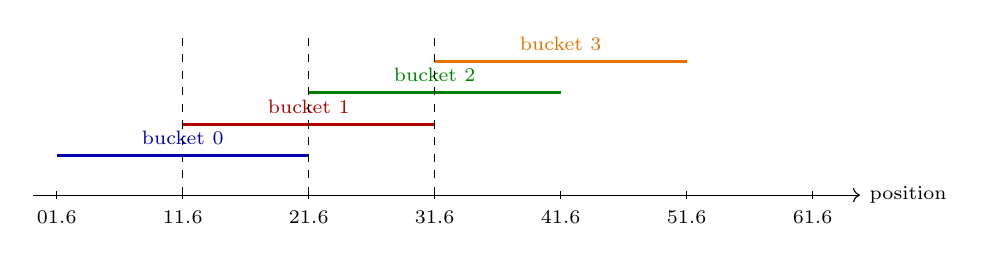
\begin{tikzpicture}[scale=1, every node/.style={font=\scriptsize}]
  \def\ell{1.6}
  \draw[->] (-0.3,0) -- (6*\ell+0.6,0) node[right] {position};
  \foreach \i in {0,...,6} {
    \draw (\i*\ell,0.05) -- (\i*\ell,-0.05);
    \node[below] at (\i*\ell,-0.08) {$\i\ell$};
  }
  \draw[very thick, blue!70!black] (0,0.5) -- (2*\ell,0.5) node[midway,above] {bucket 0};
  \draw[very thick, red!70!black] (1*\ell,0.9) -- (3*\ell,0.9) node[midway,above] {bucket 1};
  \draw[very thick, green!50!black] (2*\ell,1.3) -- (4*\ell,1.3) node[midway,above] {bucket 2};
  \draw[very thick, orange!90!black] (3*\ell,1.7) -- (5*\ell,1.7) node[midway,above] {bucket 3};
  \draw[dashed] (1*\ell,0) -- (1*\ell,2);
  \draw[dashed] (2*\ell,0) -- (2*\ell,2);
  \draw[dashed] (3*\ell,0) -- (3*\ell,2);
\end{tikzpicture}
\caption{Bucket geometry: each bucket spans $2\ell$, consecutive buckets overlap by $\ell$
(50\%). A hit at position $p \in [\ell, 2\ell)$ (e.g.\ the overlap region between buckets 0 and 1)
is attributed to \emph{both} bucket 0 and bucket 1.}
\end{figure}

\paragraph{Why 50\% overlap.} Without overlap, a true alignment straddling a bucket boundary would
have its matches split roughly in half between two non-overlapping buckets, and neither alone
would score well even though the true alignment is real and strong. With 50\% overlap, \emph{any}
true alignment of length up to $\ell$ is guaranteed to be fully contained within at least one
bucket (the one aligned with its start, or its neighbor), at the cost of roughly doubling the
number of (hit, bucket) attributions that must be tracked. This is directly analogous to why
minimizer schemes (\S\ref{sec:minimizers}) guarantee window coverage --- it is the same
``don't let a real signal fall in a seam'' concern, solved geometrically instead of via a
window-based sampling guarantee.

\subsection{Choosing $\ell$: the bucket half-length}
\label{sec:bucket-halflen}

$\ell$ is set once per read, to the read's own sketch size $m$ (or, under \code{abs\_pos}, the
read's raw nucleotide length) --- i.e., \textbf{a bucket is sized to be exactly as wide as the
read it's being used for}, so that a bucket can plausibly contain one full copy of the read's
alignment. A minimum half-length $\ell_{\min}=5$ is enforced as a sanity floor (extremely short
reads/sketches are rejected as unmappable rather than creating degenerate buckets).

\section{\code{Buckets}: the primary per-run accumulator}
\label{sec:buckets-struct}

One \code{Buckets} instance is created once per mapping run (not per read) and \code{clear()}'d
between reads (\S\ref{sec:buckets-clear}) --- this reuses its backing storage rather than
reallocating per read.

\begin{center}
\begin{tabularx}{\textwidth}{@{}llX@{}}
\toprule
\textbf{Field} & \textbf{Type} & \textbf{Meaning} \\
\midrule
\code{halflen} & int & Current read's $\ell$ (\S\ref{sec:bucket-halflen}); reset every read. \\
\code{i} & int & Index of the next seed (into the current read's seed list) not yet propagated to
  every touched bucket's own \code{.i} counter (\S\ref{sec:bucket-propagate}). \\
\code{seeds} & int & Seed-occurrence budget consumed so far, mirrored into every touched bucket. \\
\code{buckets} & one \code{Vec<BucketContent>} per segment & Flat, directly-indexed storage:
  \code{buckets[segm\_id][b]} is that bucket's running \code{BucketContent}
  (\S\ref{sec:type-bucketcontent}), pre-sized to $\lceil \mathit{segment\_length}/\ell_{\min}
  \rceil + 2$ slots at construction time so that it is large enough for \emph{any} valid $\ell \ge
  \ell_{\min}$ used later. \\
\code{non\_empty\_buckets\_with\_repeats} & \code{Vec<BucketLoc>} & Every \code{BucketLoc} touched
  since the last \code{clear()}, \textbf{with duplicates} (a bucket touched by 5 different hits
  appears 5 times) --- deduplicated only when \code{get\_sorted\_buckets} is called
  (\S\ref{sec:get-sorted-buckets}). Doubling as the undo-log for \code{clear()}. \\
\bottomrule
\end{tabularx}
\end{center}

\begin{notebox}
The reference C++ caps the number of reference segments at a hardcoded constant
(\code{MAX\_SEGMENTS = 100}), throwing at construction time for larger references. This reads as
an arbitrary implementation limit, not an intentional one --- draft/scaffolded genome assemblies
routinely have thousands of small contigs. A from-scratch implementation should size
\code{buckets} to the reference's \emph{actual} segment count instead of imposing any fixed cap.
\end{notebox}

\subsection{\code{clear()}}
\label{sec:buckets-clear}

\begin{algobox}{title={\code{Buckets::clear}()}}
\begin{verbatim}
i := 0
seeds := 0
for (segm_id, b) in non_empty_buckets_with_repeats:
    buckets[segm_id][b] := BucketContent::default()   # reset just the touched slots
non_empty_buckets_with_repeats.clear()
\end{verbatim}
\end{algobox}

Only slots that were actually touched are reset (tracked via the repeats log) --- this is
$O(\text{touched slots in the previous read})$, not $O(\text{reference size})$, which matters
because the vast majority of a genome-scale reference's buckets are never touched by any single
read.

\subsection{\code{add\_to\_pos} and \code{add\_to\_bucket}}

\begin{algobox}{title={\code{add\_to\_pos}(hit, content) / \code{add\_to\_bucket}(loc, content)}}
\begin{verbatim}
function add_to_pos(hit, content):
    b := (abs_pos ? hit.r : hit.tpos) / halflen        # integer division
    buckets[hit.segm_id][b] += content                  # BucketContent's additive merge
    log(hit.segm_id, b)
    if b > 0:
        buckets[hit.segm_id][b-1] += content             # 50% overlap: also touches predecessor
        log(hit.segm_id, b-1)

function add_to_bucket(loc, content):
    buckets[loc.segm_id][loc.b] += content
    log(loc.segm_id, loc.b)
\end{verbatim}
\end{algobox}

\code{add\_to\_pos} is the geometry-aware entry point (a raw hit maps to exactly one primary
bucket $b$, plus its overlap-neighbor $b{-}1$, per \S\ref{sec:bucket-geometry}); \code{
add\_to\_bucket} is a direct write to an already-known bucket location, used when the caller has
already done bucket-location arithmetic itself (\S\ref{sec:match-seeds}, for multi-hit seeds).

\subsection{Propagating the seed cursor: \code{propagate\_seeds\_to\_buckets}}
\label{sec:bucket-propagate}

\begin{algobox}{title={\code{propagate\_seeds\_to\_buckets}()}}
\begin{verbatim}
for (segm_id, b) in non_empty_buckets_with_repeats:
    buckets[segm_id][b].i := i
    buckets[segm_id][b].seeds := seeds
\end{verbatim}
\end{algobox}

Called once, after \code{match\_seeds} (\S\ref{sec:match-seeds}) has consumed the full seed
budget $S$ for the read: every touched bucket's own \code{.i}/\code{.seeds} counters are
initialized to the \emph{global} cursor position, so that incremental pruning
(Chapter~\ref{ch:pruning}) can resume extending each bucket from exactly where uniform seed
consumption left off, without having to replay every seed from scratch per bucket.

\subsection{\code{get\_sorted\_buckets}}
\label{sec:get-sorted-buckets}

\begin{algobox}{title={\code{get\_sorted\_buckets}()}}
\begin{verbatim}
sort non_empty_buckets_with_repeats by (segm_id, b)
deduplicate consecutive equal entries
result := [ (loc, buckets[loc.segm_id][loc.b]) for loc in deduplicated ]
sort result by content.matches descending
return result
\end{verbatim}
\end{algobox}

This is the hand-off point to pruning/refinement (Chapters~\ref{ch:pruning}--\ref{ch:scoring}):
buckets are visited \textbf{most-matches-first}, so that the best candidates raise the acceptance
threshold as early as possible, making the seed-heuristic bound (\S\ref{sec:seed-heuristic-theory})
prune later (worse) buckets even more aggressively.

\begin{notebox}
The reference C++ uses \code{std::sort}, whose relative order for \emph{tied} match counts is
unspecified (and not even guaranteed stable across compiler/standard-library versions). A
from-scratch implementation using a stable sort will therefore not, in general, reproduce the
exact tie-broken order the reference binary happens to produce on any given build --- this is a
property of the reference implementation, not a target worth chasing; downstream results only
depend on tie-breaking when two buckets score \emph{exactly} equally, which is rare in practice
and does not affect which bucket is ultimately reported as long as the final selection compares
scores explicitly (which it does, \S\ref{sec:match-rest}).
\end{notebox}

\section{\code{BucketsHash}: ephemeral scratch structure for one multi-hit seed}
\label{sec:buckets-hash}

A second, hash-map-backed structure with the same \code{add\_to\_pos} geometry (keyed by
\code{BucketLoc} directly, rather than a flat per-segment array) is used \emph{only} as short-lived
scratch space, local to processing a single seed with more than one reference hit
(\S\ref{sec:match-seeds}) --- never as an alternative backing store for the main per-run
\code{Buckets}. It needs no \code{clear()}/undo-log machinery since a fresh instance is created
per multi-hit seed and discarded immediately after.

\section{\code{match\_seeds}: populating buckets from the seed budget}
\label{sec:match-seeds}

\paragraph{Input.} The read's sorted seed list (Chapter~\ref{ch:seeding}), the (per-run,
just-cleared) \code{Buckets}, and the seed budget $S$ (occurrences, \S\ref{sec:seed-budget}).

\paragraph{Output.} None (mutates \code{buckets} in place); also returns/accumulates the total
seed-match count for diagnostics.

\begin{algobox}{title={\code{match\_seeds}(seeds, buckets, S)}}
\begin{verbatim}
while buckets.i < len(seeds) and buckets.seeds < S:
    seed := seeds[buckets.i]
    if seed.hits_in_t > 0:
        if seed.hits_in_t == 1:
            hit := index.h2single[seed.kmer.h]
            content := BucketContent(matches=1, seeds=0,
                                      codirection = (hit.strand==seed.kmer.strand) ? +1 : -1,
                                      r_min=hit.r, r_max=hit.r)
            buckets.add_to_pos(hit, content)
        else:
            # De-duplicate this *one* seed's own multiple reference hits into
            # per-bucket contributions *before* merging into the shared
            # Buckets store, so that a seed occurring k times inside one
            # bucket only ever contributes min(k, occs_in_p) matches to it
            # (a seed cannot match "more than itself" in a single bucket).
            scratch := BucketsHash(halflen = buckets.halflen)
            for hit in index.h2multi[seed.kmer.h]:
                c := BucketContent(matches=1, seeds=0,
                                    codirection = (hit.strand==seed.kmer.strand) ? +1 : -1,
                                    r_min=hit.r, r_max=hit.r)
                scratch.add_to_pos(hit, c)
            for (loc, c) in scratch.buckets:
                clamped := BucketContent(matches = min(c.matches, seed.occs_in_p), seeds=0,
                                          codirection=c.codirection,
                                          r_min=c.r_min, r_max=c.r_max)
                buckets.add_to_bucket(loc, clamped)
    buckets.seeds += seed.occs_in_p
    buckets.i += 1
\end{verbatim}
\end{algobox}

\paragraph{Why the extra de-duplication pass for multi-hit seeds.} A seed with, say,
\code{occs\_in\_p}$=2$ (occurs twice in the read) and \code{hits\_in\_t}$=5$ (occurs 5 times in
the reference) could have several of those 5 reference hits fall inside the \emph{same} bucket.
Without capping, that bucket would be credited with up to 5 matches from a seed that only truly
occurs twice in the read --- overcounting. The scratch structure first tallies, per bucket, how
many of this one seed's reference hits land there, then clamps that tally to
\code{occs\_in\_p} before merging into the shared \code{Buckets} store, guaranteeing a single
seed can never contribute more matches to any one bucket than it actually occurs in the read.

\section{Reference C++ implementation}

\begin{lstlisting}[style=cppstyle,caption={\code{match\_seeds} and \code{Buckets::add\_to\_pos}, \texttt{src/shmap.h} \& \texttt{src/buckets.h}}]
void match_seeds(const Seeds &p_unique, BucketsType &B, qpos_t S) {
    for (; B.i < (qpos_t)p_unique.size() && B.seeds < S; B.i++) {
        Seed seed = p_unique[B.i];
        if (seed.hits_in_T > 0) {
            if (seed.hits_in_T == 1) {
                const auto &hit = tidx.h2single.at(seed.kmer.h);
                BucketContent content(1, 0, hit.strand == seed.kmer.strand ? 1 : -1, hit.r, hit.r);
                B.add_to_pos(hit, content);
            } else {
                BucketsHash<abs_pos> b2m(B.halflen);
                for (const auto &hit: tidx.h2multi.at(seed.kmer.h)) {
                    BucketContent content(1, 0, hit.strand == seed.kmer.strand ? 1 : -1, hit.r, hit.r);
                    b2m.add_to_pos(hit, content);
                }
                for (auto it = b2m.buckets.begin(); it != b2m.buckets.end(); ++it) {
                    BucketContent content(min(it->second.matches, seed.occs_in_p), 0,
                                           it->second.codirection, it->second.r_min, it->second.r_max);
                    B.add_to_bucket(it->first, content);
                }
            }
        }
        B.seeds += seed.occs_in_p;
    }
}

void add_to_pos(const Hit& hit, const BucketContent &content) {
    qpos_t b = (abs_pos ? hit.r : hit.tpos) / halflen;
    buckets[hit.segm_id][b] += content;
    non_empty_buckets_with_repeats.push_back(BucketLoc(hit.segm_id, b));
    if (b > 0) {
        buckets[hit.segm_id][b-1] += content;
        non_empty_buckets_with_repeats.push_back(BucketLoc(hit.segm_id, b-1));
    }
}
\end{lstlisting}

\section{Complexity}

Populating buckets from $S$ consumed seed occurrences costs $O(S \cdot \bar d)$, where $\bar d$ is
the average reference-hit count of a consumed seed (bounded by \code{-M} when set,
\S\ref{sec:max-matches}). \code{get\_sorted\_buckets} costs $O(u \log u)$ where $u$ is the number
of distinct buckets touched this read --- typically far smaller than the reference size, since
only buckets that received at least one seed match are ever touched at all.

\chapter{Seed-Heuristic Pruning}
\label{ch:pruning}

This chapter gives the exact implementation of the pruning bound whose theory was developed in
\S\ref{sec:seed-heuristic-theory}. Three pieces compose: the bound formula itself (\code{hseed}),
an incremental bucket-extension step (\code{matches\_in\_bucket}) that pulls in \emph{one more}
seed's worth of information about a specific bucket on demand, and the driving loop
(\code{seed\_heuristic\_pass}) that alternates ``check the bound'' and ``extend'' until the bucket
is either proven prunable or fully caught up with all consumed seeds.

\section{\code{hseed}: the bound formula}

\[
  h_{\mathrm{seed}}(m,\ \mathit{seeds},\ \mathit{matches}) = 1 - \frac{\mathit{seeds} -
  \mathit{matches}}{m}
\]
with $m$ the read's sketch size, and $\mathit{seeds}/\mathit{matches}$ the bucket's own running
counters (\S\ref{sec:type-bucketcontent}). See \S\ref{sec:seed-heuristic-theory} for the proof
that this is a valid, monotonically-tightening upper bound on the bucket's final containment
score.

\section{\code{matches\_in\_bucket}: extending a bucket by one more seed}
\label{sec:matches-in-bucket}

\paragraph{Input.} The shared \code{Buckets} store (read-only here), a specific
\code{BucketLoc}, that bucket's own (mutable) running \code{BucketContent}, and the next seed
\code{s} to check against it.

\paragraph{Output.} None; mutates the passed \code{BucketContent} in place: increments
\code{.seeds} by \code{s.occs\_in\_p} unconditionally, and increments \code{.matches} (plus
updates \code{.codirection}/\code{.r\_min}/\code{.r\_max}) by however many of \code{s}'s reference
hits fall inside this bucket's span.

\begin{algobox}{title={\code{matches\_in\_bucket}(buckets, loc, content, s)}}
\begin{verbatim}
content.seeds += s.occs_in_p
if s.hits_in_t == 0:
    return                                     # nothing to add
if s.hits_in_t == 1:
    hit := index.h2single[s.kmer.h]
    pos := abs_pos ? hit.r : hit.tpos
    if buckets.begin(loc) <= pos < buckets.end(loc):
        content.matches += 1
        content.codirection += (hit.strand == s.kmer.strand) ? 1 : -1
        content.r_min := min(content.r_min, hit.r)
        content.r_max := max(content.r_max, hit.r)
else:  # s.hits_in_t > 1
    hits := index.h2multi[s.kmer.h]             # sorted by (segm_id, r); see 6.3
    start := binary_search first hit with (segm_id, pos) >= (loc.segm_id, buckets.begin(loc))
    matches := 0
    for hit in hits[start:]:
        pos := abs_pos ? hit.r : hit.tpos
        if not (hit.segm_id == loc.segm_id and pos < buckets.end(loc)):
            break                                # sorted: no further hit can match either
        matches += 1
        content.codirection += (hit.strand == s.kmer.strand) ? 1 : -1
        content.r_min := min(content.r_min, hit.r)
        content.r_max := max(content.r_max, hit.r)
    content.matches += min(matches, s.occs_in_p)  # same per-seed clamp as match_seeds (8.5)
\end{verbatim}
\end{algobox}

The multi-hit branch's binary search + early-break scan is exactly why \code{h2multi} lists are
kept sorted by \code{(segm\_id, r)} (\S\ref{sec:index-sort}): it lets this function cost
$O(\log d + c)$ (binary search plus $c$ = actual hits found in range) rather than $O(d)$ (scanning
every one of the seed's $d$ reference occurrences), which matters because this function may be
called many times per bucket during incremental pruning.

\section{\code{seed\_heuristic\_pass}: the driving loop}
\label{sec:seed-heuristic-pass}

\paragraph{Input.} The shared \code{Buckets}, the read's full seed list, the read's sketch size
$m$, the bucket being evaluated (location + its running content, mutable), a mutable slot to
report the bound value achieved, and the current acceptance threshold \code{thr} (the higher of
the CLI's $\theta$ and the current best-known score, \S\ref{sec:match-rest}).

\paragraph{Output.} Boolean: \code{true} if the bucket \emph{survives} pruning (its bound stays
$\ge$ \code{thr} after being extended with every seed consumed so far), \code{false} the instant
its bound drops below \code{thr}.

\begin{algobox}{title={\code{seed\_heuristic\_pass}(buckets, seeds, m, loc, content, \&sh, thr)}}
\begin{verbatim}
if no_bucket_pruning:               # -P flag: pruning disabled entirely
    return true

loop:
    sh := hseed(m, content.seeds, content.matches)
    if sh < thr:
        return false                              # proven prunable: stop immediately
    if content.i >= len(seeds):
        break                                      # caught up with every consumed seed: survives
    matches_in_bucket(buckets, loc, content, seeds[content.i])
    content.i += 1
return true
\end{verbatim}
\end{algobox}

\paragraph{Why check the bound \emph{before} each extension, not after.} Checking first means a
bucket that is already unsalvageable (e.g.\ its very first few seeds were all misses) is rejected
in $O(1)$ --- zero calls to \code{matches\_in\_bucket} --- rather than paying for at least one
extension step before discovering the same conclusion. Because \code{hseed} only ever decreases
or holds steady as \code{content.i} advances (\S\ref{sec:seed-heuristic-theory}), checking first
never risks accepting a bucket the ``check after'' ordering would have rejected, or vice versa ---
the two orderings are behaviorally equivalent except for this one-step efficiency difference.

\paragraph{Why \code{content.i} can start anywhere.} Recall from
\S\ref{sec:bucket-propagate} that every bucket's \code{.i}/\code{.seeds} counters are initialized,
once, to the \emph{global} cursor value reached after \code{match\_seeds} finished consuming the
full budget $S$. So the very first call to \code{seed\_heuristic\_pass} for a given bucket starts
its incremental extension already caught up to $S$ (\code{content.i} $= S$'s position in the seed
list already, assuming that bucket was touched at all during \code{match\_seeds}) --- extension
only ever goes \emph{further}, past the seeds that were used to build the buckets in the first
place, giving each surviving bucket a chance to be confirmed/rejected using \emph{more} evidence
than the initial seeding pass alone provided, without redoing any of that initial work.

\section{The \code{no\_bucket\_pruning} flag (\code{-P})}

When set, \code{seed\_heuristic\_pass} degenerates to an unconditional \code{return true}: every
bucket that survived \code{get\_sorted\_buckets} proceeds straight to full refinement
(Chapter~\ref{ch:scoring}), with no early rejection at all. This is strictly slower and produces
identical \emph{results} to the pruned path (pruning is provably conservative, per
\S\ref{sec:seed-heuristic-theory} --- it can only ever discard buckets that could not have won
anyway) — its purpose is as a ground-truth oracle for testing/benchmarking the pruning logic
itself, and as a fallback if a from-scratch implementation's pruning bound is ever suspected of a
bug: run both, and any discrepancy in the winning bucket indicates a pruning bug, not a scoring
one.

\section{Reference C++ implementation}

\begin{lstlisting}[style=cppstyle,caption={\code{hseed}, \code{matches\_in\_bucket}, \code{seed\_heuristic\_pass}, \texttt{src/shmap.h}}]
double hseed(qpos_t p, qpos_t seeds, qpos_t matches) {
    return 1.0 - double(seeds - matches) / p;
}

void matches_in_bucket(const BucketsType &B, const BucketLoc &b, BucketContent *bucket, const Seed &s) const {
    bucket->seeds += s.occs_in_p;
    if (s.hits_in_T == 0) {
        ;
    } else if (s.hits_in_T == 1) {
        const auto &hit = tidx.h2single.at(s.kmer.h);
        if (abs_pos ? B.begin(b) <= hit.r    && hit.r    < B.end(b)
                    : B.begin(b) <= hit.tpos && hit.tpos < B.end(b)) {
            bucket->matches += 1;
            bucket->codirection += hit.strand == s.kmer.strand ? 1 : -1;
            bucket->r_min = min(bucket->r_min, hit.r);
            bucket->r_max = max(bucket->r_max, hit.r);
        }
    } else if (s.hits_in_T > 1) {
        const auto &hits = tidx.h2multi.at(s.kmer.h);
        auto it = lower_bound(hits.begin(), hits.end(), B.begin(b), [&b](const Hit &hit, rpos_t pos) {
            if (hit.segm_id != b.segm_id) return hit.segm_id < b.segm_id;
            return abs_pos ? hit.r < pos : hit.tpos < pos;
        });
        rpos_t matches = 0;
        for (; it != hits.end(); ++it) {
            if (abs_pos) { if (!(it->segm_id == b.segm_id && it->r < B.end(b))) break; }
            else         { if (!(it->segm_id == b.segm_id && it->tpos < B.end(b))) break; }
            matches += 1;
            bucket->codirection += it->strand == s.kmer.strand ? 1 : -1;
            bucket->r_min = min(bucket->r_min, it->r);
            bucket->r_max = max(bucket->r_max, it->r);
        }
        bucket->matches += min(matches, s.occs_in_p);
    }
}

bool seed_heuristic_pass(const BucketsType &B, const Seeds &p_unique, qpos_t m, const BucketLoc &b,
                          BucketContent *bucket, double *sh, double thr) {
    if (!no_bucket_pruning) {
        while (1) {
            *sh = hseed(m, bucket->seeds, bucket->matches);
            if (*sh < thr) return false;
            if (bucket->i >= (qpos_t)p_unique.size()) break;
            matches_in_bucket(B, b, bucket, p_unique[bucket->i]);
            bucket->i++;
        }
    }
    return true;
}
\end{lstlisting}

\section{Worked example}

Suppose $m=100$ (read sketch size), $\mathit{thr}=0.9$, and a candidate bucket's running counters
after seeding are $\mathit{seeds}=40,\ \mathit{matches}=38$. Then $h_{\mathrm{seed}} = 1 -
(40-38)/100 = 0.98 \ge 0.9$: survives, extend further. Suppose the next three consumed seeds (each
\code{occs\_in\_p}$=1$) contribute $0, 1, 0$ matches to this bucket respectively:
after seed 1, $\mathit{seeds}=41,\mathit{matches}=38 \Rightarrow h_{\mathrm{seed}}=0.97$; after
seed 2, $\mathit{seeds}=42,\mathit{matches}=39 \Rightarrow h_{\mathrm{seed}}=0.97$; after seed 3,
$\mathit{seeds}=43,\mathit{matches}=39 \Rightarrow h_{\mathrm{seed}}=0.96$ --- still above
$0.9$, so this bucket keeps surviving each check. If instead six consecutive misses had occurred
($\mathit{seeds}$ climbing to $46$, $\mathit{matches}$ frozen at $38$), $h_{\mathrm{seed}} = 1 -
8/100 = 0.92$, still surviving; a seventh miss would give $1-9/100=0.91$, an eighth $0.90$ (still
$\ge$, survives), a ninth $0.89 < 0.9$: \textbf{pruned} at that point, having spent only 9
incremental extension calls to conclusively rule out a bucket that (if fully scored) might have
needed to examine every remaining position in its span.

\chapter{Refinement and Scoring}
\label{ch:scoring}

Buckets that survive pruning (Chapter~\ref{ch:pruning}) are handed to \emph{refinement}: compute
an exact similarity score, and the precise matched sub-interval, for the bucket. This chapter
covers all four scoring metrics (\S\ref{sec:metric-axis}), the two-pointer sliding-window sweep
that underlies \code{Containment}/\code{Jaccard} scoring, the LCS-based alternative, and
\code{match\_rest}, the procedure that ties refinement into a best/second-best search over all of
a read's surviving buckets.

\section{The \code{diff\_hist} bookkeeping device}
\label{sec:scoring-sliding-window}

Every sliding-window sweep in this chapter maintains a shared per-read map \code{diff\_hist}:
\code{hash} $\to$ \code{remaining budget}, initialized once per read from each seed's
\code{occs\_in\_p} (how many times that $k$-mer occurs in the read). As the sweep's right (or
left) boundary crosses a reference position whose $k$-mer hash is a read seed, the corresponding
budget entry is decremented (window grows) or incremented (window shrinks) by exactly one, and
the \emph{sign} of the result after a decrement determines whether that occurrence is
countable as part of the intersection:
\begin{itemize}[nosep]
  \item Decrementing (window grows, position enters): if the value \emph{after} decrementing is
    still $\ge 0$, this occurrence is a legitimate, not-yet-used match --- count it, and record
    that it was counted (so the corresponding increment, when the window later shrinks past it,
    knows to un-count it).
  \item Incrementing (window shrinks, position leaves): if the value \emph{after} incrementing is
    $\ge 1$, this position had previously been counted --- un-count it.
\end{itemize}
This lets a sliding window maintain an exact intersection-with-multiplicity count in $O(1)$
amortized per boundary move, correctly handling repeated $k$-mers (a hash occurring 3 times in
the read can be ``used up'' by at most 3 reference positions inside the current window, no
matter how many more copies of that hash the reference bucket actually contains) --- this is the
\emph{multiset} intersection a containment/Jaccard estimate needs (\S\ref{sec:fracminhash-theory}),
not a plain set intersection.

\begin{notebox}
Because a window can shrink and regrow over the same reference position multiple times as the
sweep's left boundary advances, \code{diff\_hist} values legitimately go negative
\emph{transiently} (a decrement can push a shared hash's budget below what's currently
``available'' if multiple reference positions inside the window share that hash but the read only
has fewer occurrences) --- this is expected and exactly what the $\ge 0$ / $\ge 1$ sign checks are
designed to handle correctly; do not add an assertion that rejects negative values.
\end{notebox}

\section{\code{SHMapper}'s own \code{bestFixedLength}: the main refinement sweep}
\label{sec:best-fixed-length}

This is the function that actually refines \code{Containment}/\code{Jaccard} buckets in the main
mapping path (there is a second, differently-shaped function with the same name used only by the
ground-truth diagnostic path, \S\ref{sec:matcher-best-fixed-length} --- keep them distinct).

\paragraph{Input.} The reference segment (its full sketch), a window \code{[from, to)} to sweep
(the bucket's own span, from \code{buckets.begin}/\code{end}), the read's seed lookup table
(hash $\to$ \code{Seed}), \code{diff\_hist} (mutable, shared across the whole read's refinement
calls), the read length minus $k$ (used as the PAF end-coordinate, not a window bound), the window
\emph{width} bound $m$ (confusingly, at the call site this is actually the read's containing
$\ell$/\code{lmax} value, not the sketch size --- see the note below), and the metric
(\code{Containment} or \code{Jaccard}).

\paragraph{Output.} A \code{Mapping} (\S\ref{sec:type-mapping}): the best-scoring sub-window
found anywhere inside \code{[from, to)}.

\begin{algobox}{title={\code{bestFixedLength}(segm, from, to, seed\_table, diff\_hist, p\_sz, m, metric)}}
\begin{verbatim}
t := segm.kmers
l := max(from, 0)
r := l
end := min(len(t), to)
best := Mapping::default()          # score = -1, beaten by any real candidate

while l < end:
    while r < end:
        # window-width check, in whichever coordinate space abs_pos selects
        if abs_pos:  if not (t[r].r < t[l].r + m): break
        else:        if not (r < l + m):           break
        if t[r].h in seed_table:
            same_strand += codirection(seed_table[t[r].h].kmer, t[r])
            if (--diff_hist[t[r].h]) >= 0:
                intersection += 1
        r += 1
    # r is now exactly one past the last position included in this window
    # for the CURRENT l -- this is the point at which it is safe to score,
    # since r has already been advanced past every included element.
    s_kmers := r - l
    score := mappingScore(intersection, m, s_kmers, metric)       # 10.2 below
    if l < r and score > best.score():
        best.update(p_start=0, p_end=p_sz-1, t_l=t[l].r, t_r=t[r-1].r,
                    segm=segm, intersection=intersection, score=score,
                    same_strand=same_strand, span=t[r-1].r - t[l].r + 1)
    if t[l].h in seed_table:
        same_strand -= codirection(seed_table[t[l].h].kmer, t[l])
        if (++diff_hist[t[l].h]) >= 1:
            intersection -= 1
    l += 1
return best
\end{verbatim}
\end{algobox}

\paragraph{\code{mappingScore}:}
\[
  \mathrm{mappingScore}(\mathit{intersection}, m, s\_sz, \mathtt{Jaccard}) =
    \frac{\mathit{intersection}}{m + s\_sz - \mathit{intersection}}, \qquad
  \mathrm{mappingScore}(\mathit{intersection}, m, s\_sz, \mathtt{Containment}) =
    \frac{\mathit{intersection}}{m}.
\]
These are exactly the FracMinHash Jaccard/containment estimators of
\S\ref{sec:fracminhash-theory}, with $m$ the read's sketch size and $s\_sz$ the current window's
$k$-mer count.

\begin{notebox}
\label{sec:m-vs-psz-confusion}
At the actual call site (\S\ref{sec:find-best-mapping}), this function's \code{p\_sz} parameter
receives \emph{read length minus $k$}, and its \code{m} parameter receives $\mathit{lmax}$ (the
bucket half-length $\ell$), \emph{not} the read's sketch size in either case, despite parameter
names that suggest otherwise at a casual read. This is not a bug --- $\ell$ was chosen
(\S\ref{sec:bucket-halflen}) to equal the read's sketch size in the default (non-\code{abs\_pos})
configuration, so the values coincide numerically for the common case, but a from-scratch
implementation should pass the value that is actually semantically the ``window-width bound and
Jaccard/containment denominator'' at this call site, not necessarily whatever local variable
happens to be named \code{m} in a hasty transcription. Name the parameter for what it does,
not what one caller happens to pass.
\end{notebox}

\paragraph{Why scoring happens \emph{after} the inner \code{while} loop exits, not inside it.}
This is the single most important structural detail in this function, and the source of a real
bug in the ground-truth-only sibling function discussed in \S\ref{sec:matcher-best-fixed-length}:
after the inner loop's normal exit, \code{r} is \emph{exactly one past} the last position that
was ever included in the window for the current \code{l} (standard half-open-range convention:
the loop only stops once its own condition fails, having already processed and advanced past
every element that satisfied it). So \code{t[r-1]} unambiguously means ``the last element
actually in the window'', consistent with what \code{intersection} counts. Any refinement sweep
that instead scores \emph{mid-loop} (before the equivalent exit has happened) must use the
\emph{current}, not-yet-advanced index for both the score's span \emph{and} its use of
\code{intersection}, or the two will disagree --- see \S\ref{sec:matcher-best-fixed-length} for a
concrete case where the reference implementation gets exactly this wrong.

\section{\code{findBestMapping}: dispatching on metric}
\label{sec:find-best-mapping}

\begin{algobox}{title={\code{findBestMapping}(buckets, loc, content, seed\_table, diff\_hist, p\_sz, m, lmax, sh, metric, k)}}
\begin{verbatim}
switch metric:
  case bucket_SH:
    # Degenerate/cheap: reuse the seed-heuristic bound itself as the score,
    # with the bucket's own tracked position range as the matched interval.
    # No refinement sweep at all -- O(1) given the bucket's content.
    best := Mapping(p_start=0, p_end=p_sz-1, t_l=content.r_min, t_r=content.r_max,
                    segm=ref_segment(loc.segm_id), intersection=content.matches,
                    score=sh, same_strand=content.codirection,
                    span=content.r_max - content.r_min)

  case bucket_LCS:
    lcs_len := lcs(ref_segment(loc.segm_id).kmers, buckets, loc, seed_table)   # 10.4
    score := lcs_len / m
    best := Mapping(p_start=0, p_end=p_sz-1, t_l=content.r_min, t_r=content.r_max,
                    segm=ref_segment(loc.segm_id), intersection=content.matches,
                    score=score, same_strand=content.codirection,
                    span=content.r_max - content.r_min)

  case Containment or Jaccard:
    best := bestFixedLength(ref_segment(loc.segm_id), buckets.begin(loc), buckets.end(loc),
                             seed_table, diff_hist, p_sz - k, lmax, metric)

best.set_bucket(loc)
best.set_sh(sh)
return best
\end{verbatim}
\end{algobox}

\section{The \code{bucket\_LCS} metric: longest common subsequence chain score}
\label{sec:lcs-implementation}

\paragraph{Motivation.} Containment/Jaccard scoring treats every matched $k$-mer equally,
regardless of whether the matches are mutually \emph{co-linear} (consistent with one real
alignment) or scattered (an artifact of repeats). \code{bucket\_LCS} instead scores a bucket by
how long a co-linear chain of matches it contains, per \S\ref{sec:lis-theory}.

\subsection{\code{lcs\_get\_ppos\_in\_t}: collecting the position sequence}

\begin{algobox}{title={\code{lcs\_get\_ppos\_in\_t}(t, buckets, loc, seed\_table)}}
\begin{verbatim}
ppos_in_t := []
for l in buckets.begin(loc) .. min(len(t), buckets.end(loc)) - 1:
    if t[l].h in seed_table:
        for ppos in seed_table[t[l].h].pmatches:      # Section 4.4: all read positions sharing this hash
            ppos_in_t.append(ppos)
return ppos_in_t
\end{verbatim}
\end{algobox}

This produces, in increasing reference-position order, the sequence of read-side positions that
each reference $k$-mer inside the bucket matches (with repetition, if a hash occurs multiple times
in the read). A long increasing run in this sequence is a long co-linear chain.

\subsection{\code{lcs\_get\_lis}: patience-sorting LIS length}
\label{sec:lcs-lis}

Exactly the classic $O(n\log n)$ algorithm of \S\ref{sec:lis-theory}:

\begin{algobox}{title={\code{lcs\_get\_lis}(ppos\_in\_t)}}
\begin{verbatim}
tails := []                       # tails[i] = smallest tail of an increasing run of length i+1
for x in ppos_in_t:
    lo, hi := -1, len(tails)
    while lo + 1 < hi:
        mid := (lo + hi) / 2
        if tails[mid] < x: lo := mid
        else:              hi := mid
    if hi == len(tails): tails.append(x)
    else:                 tails[hi] := x
return tails                       # len(tails) is the LIS length
\end{verbatim}
\end{algobox}

\subsection{\code{lcs}: combining forward and reverse}

\begin{algobox}{title={\code{lcs}(t, buckets, loc, seed\_table)}}
\begin{verbatim}
ppos_in_t := lcs_get_ppos_in_t(t, buckets, loc, seed_table)
forward_len := len(lcs_get_lis(ppos_in_t))
reverse(ppos_in_t)
reverse_len := len(lcs_get_lis(ppos_in_t))
return max(forward_len, reverse_len)
\end{verbatim}
\end{algobox}

Running LIS on the \emph{reversed} position sequence finds the longest \emph{decreasing} run of
the original --- i.e., the longest chain co-linear on the opposite strand. Taking the max of both
directions makes this metric strand-agnostic without needing to know the winning strand ahead of
time.

\section{\code{match\_rest}: best and second-best search}
\label{sec:match-rest}

\paragraph{Input.} All of a read's sorted, surviving buckets; the read's seed list, seed table,
and \code{diff\_hist}; an acceptance threshold \code{thr}; an optional ``forbidden'' \code{Mapping}
(when searching for the second-best, this is the best mapping already found, so that a
near-duplicate of it is excluded, \S\ref{sec:overlap-exclusion}); and \code{max\_overlap} (CLI
\code{-o}).

\paragraph{Output.} The single best \code{Mapping} across all surviving buckets that both beats
\code{thr} and (if \code{forbidden} is given) does not overlap it by more than
\code{max\_overlap}; or none, if no bucket qualifies.

\begin{algobox}{title={\code{match\_rest}(p\_sz, m, lmax, seeds, buckets, sorted\_buckets, diff\_hist, seed\_table, thr, forbidden, max\_overlap, metric, k)}}
\begin{verbatim}
best := None
for (loc, content) in sorted_buckets:              # most-matches-first, Section 8.6
    sh := 1.0
    if seed_heuristic_pass(buckets, seeds, m, loc, content, &sh, thr):   # Chapter 9
        candidate := findBestMapping(buckets, loc, content, seed_table, diff_hist,
                                      p_sz, m, lmax, sh, metric, k)
        if candidate.score() > thr:
            if forbidden is None or overlap(candidate, forbidden) < max_overlap:
                thr := candidate.score()            # raise the bar for subsequent buckets
                best := candidate
return best
\end{verbatim}
\end{algobox}

\subsection{Overlap exclusion}
\label{sec:overlap-exclusion}

\[
  \mathrm{overlap}(a, b) = \begin{cases} -0.0 & \text{different segments} \\
  \dfrac{\max(0,\ \min(a.t_r,b.t_r) - \max(a.t_l,b.t_l))}{\max(a.t_r,b.t_r) - \min(a.t_l,b.t_l)}
  & \text{same segment} \end{cases}
\]
i.e., intersection-over-union of the two candidates' matched reference intervals, restricted to
same-segment pairs. A second-best candidate search rejects any bucket whose refined interval
overlaps the already-found best by $\ge \mathit{max\_overlap}$ --- without this, the ``second
best'' would routinely just be a slightly-shifted restatement of the exact same true alignment
(since neighboring, heavily-overlapping buckets, per \S\ref{sec:bucket-geometry}, often all score
similarly well against the same true locus), which would make MAPQ (Chapter~\ref{ch:mapq})
uselessly report low confidence for essentially every uniquely-mapping read.

\subsection{How the caller invokes \code{match\_rest} twice}

The per-read driver (fully assembled in Chapter~\ref{ch:end-to-end}) calls \code{match\_rest}
exactly twice: once with \code{thr}$=\theta$ (the CLI acceptance threshold) and
\code{forbidden}$=$\code{None} to find the best mapping; then, only if a best mapping was found,
a second time with \code{thr} $= \mathit{best.score()} \times (1 - \mathit{min\_diff})$ and
\code{forbidden}$=$\code{best} to find the second-best. Both calls sweep the \emph{same} sorted
bucket list and share the \emph{same} \code{diff\_hist} (which is why every refinement sweep is
required to leave \code{diff\_hist} in exactly the state it found it, \S
\ref{sec:scoring-sliding-window} --- the second call depends on that invariant holding after the
first).

\section{The ground-truth-only sibling functions, and a genuine bug}
\label{sec:matcher-best-fixed-length}

A second, narrower set of functions (grouped under a type usually called \code{Matcher}) exists
solely to support the \emph{verbose ground-truth diagnostic} output (\S\ref{sec:ground-truth},
used only with \code{-v~2}, never in the main scoring path above). It re-implements
\code{collect\_matches} (turn a bucket into an explicit list of \code{Match}es, rather than
sweeping the reference sketch directly), a \code{bestFixedLength} that sweeps that explicit list
using \code{hit.r <= l.hit.r + p\_sz} as its window bound (notably \emph{not} respecting an
\code{lmax} parameter it is nonetheless passed --- see the dead-parameter note in
Chapter~\ref{ch:defects}), and a \code{bestIncludedJaccard} that finds the best-scoring window
whose length falls within an explicit $[\ell_{\min}, \ell_{\max}]$ range (used to check, precisely,
what score the ground-truth region itself would have achieved).

\begin{bugbox}
\label{sec:defect-prevr}
\code{bestIncludedJaccard}'s two-pointer sweep scores \emph{mid-loop}, immediately after growing
the window's right boundary by one, using the position \emph{one before} the just-processed
element (an iterator idiom equivalent to \code{prev(r)}) for both the matched span and the
reported right boundary --- while \code{intersection} at that exact point \emph{already} reflects
the just-processed (current, not ``previous'') element. This is an internal inconsistency: the
score's span excludes an element that the match count includes, which can and does produce
\code{intersection > span}, violating the metric's own well-formedness invariant
($\mathit{intersection} \le s\_sz$ must hold for a containment/Jaccard ratio to stay in $[0,1]$).
The original source itself carries a \texttt{// TODO: should it be prev(r) instead?} comment on
this exact line, i.e.\ the original author flagged this specific spot as unsettled. Confirmed by
constructing a small worked example (a $\sim$50bp read against a $\sim$200bp synthetic reference)
that reliably triggers the invariant violation. Because this path has \emph{zero} automated test
coverage in the reference codebase and only ever affects a diagnostic tag (never the main PAF
output), there is no existing oracle to defer to; the internally consistent fix --- score using
the \emph{current}, just-processed right-boundary element throughout, matching what
\code{intersection} already counts, exactly as \S\ref{sec:best-fixed-length}'s ``score after the
loop exits'' pattern already does correctly --- is the recommended behavior for a from-scratch
implementation of this diagnostic feature. See Chapter~\ref{ch:defects} for the full write-up.
\end{bugbox}

\section{Complexity}

Each refinement sweep (\code{bestFixedLength} or \code{lcs}) costs $O(|\mathrm{bucket}|)$: one
linear pass over the bucket's span of the reference sketch, with $O(1)$ amortized work per
position via the \code{diff\_hist} device (\S\ref{sec:scoring-sliding-window}) or, for LCS,
$O(|\mathrm{bucket}|\log|\mathrm{bucket}|)$ owing to the patience-sorting binary search. Summed
over all buckets that survive pruning (Chapter~\ref{ch:pruning}), and since pruning is designed
to make that survivor count small and roughly independent of total reference size, total
refinement cost per read is, in practice, far closer to $O(\ell)$ (one bucket's worth of work)
than to $O(n)$ (the whole reference).

\chapter{End-to-End Algorithm}
\label{ch:end-to-end}

This chapter reassembles every module from Chapters~\ref{ch:sketching}--\ref{ch:scoring} into the
two top-level routines that actually run: \code{map\_reads} (once per program invocation) and
\code{map\_read} (once per read). This is the single most useful reference for a from-scratch
implementation, and is written in its \emph{corrected} form (i.e., incorporating the fixes from
Chapter~\ref{ch:defects} where they affect observable behavior) with explicit call-outs at every
point a decision was made about a defect in the reference source.

\section{\code{map\_reads}: the outer loop}

\begin{algobox}{title={\code{map\_reads}(index, reads\_file, params)}}
\begin{verbatim}
open unmapped_out  := params.params_file + ".unmapped.paf"  if params.params_file is set else None
open paulout       := params.params_file + ".paul.tsv"      if params.params_file is set
                                                                and params.verbose >= 2 else None
buckets := Buckets::new(index)             # allocated once, cleared per read (Section 8.2.1)
run_wide_counters := Counters::new()
run_wide_timers   := Timers::new()

for (query_id, read_seq) in read_fasta(reads_file):
    run_wide_counters.inc("reads")
    per_read_counters, per_read_timers := map_read(index, params, read_seq, query_id,
                                                     buckets, unmapped_out, paulout)
    run_wide_counters += per_read_counters      # accumulate into run totals
    run_wide_timers   += per_read_timers

print_summary_statistics(run_wide_counters, run_wide_timers)
\end{verbatim}
\end{algobox}

\begin{notebox}
Each read is processed with its own fresh, fully-reset per-read counters (see the boxed
correction in \S\ref{sec:map-read-counters} below) that are merged into the run-wide totals
\emph{after} that read finishes --- this merge-after-each-read pattern is what lets a single PAF
line's diagnostic tags (\S\ref{ch:output}) report purely this-read quantities while the
end-of-run summary still reports correct totals across all reads.
\end{notebox}

\section{\code{map\_read}: per-read driver}
\label{sec:map-read}

\subsection{Counter initialization}
\label{sec:map-read-counters}

\begin{bugbox}
The reference C++ does \emph{not} actually reset its per-read counters object between reads: the
call that would clear it (\code{C.clear()}) is commented out, and the subsequent
re-initialization list names only a subset of the counters the function goes on to increment ---
seven counters, including \code{total\_matches} (which feeds directly into the \emph{live}
\code{total\_matches:i:}/\code{match\_inefficiency:f:} PAF tags, not just an end-of-run summary),
are left to accumulate, unreset, across every read a single mapper instance processes, compounding
further every time the (also unreset) running total is merged into the run-wide counters after
each read. The correct, obviously-intended behavior --- and the one specified below --- is to
\textbf{fully reset all per-read counters at the start of every read}, with every counter name the
function goes on to touch pre-registered at zero (so that end-of-read diagnostic reads never fail
on a genuinely-never-incremented counter, e.g.\ \code{mapq60} for a read with a low-confidence
mapping). See Chapter~\ref{ch:defects} for the full analysis and the complete list of affected
counter names.
\end{bugbox}

\begin{algobox}{title={\code{map\_read} --- part 1: sketch, seed, prepare}}
\begin{verbatim}
C := Counters::new()                 # fresh, fully-reset every read (see box above)
T := Timers::new()
buckets.clear()

p := sketcher.sketch(read_seq)                       # Chapter 5
m := len(p)                                            # read's sketch size
C.inc("read_len", len(read_seq))

p_unique := unique_elements_with_info(p)              # Chapter 7; rarest-hit-first

seed_table := {}          # hash -> Seed
diff_hist  := {}          # hash -> remaining occurrence budget
possible_matches := 0
for seed in p_unique:
    seed_table[seed.kmer.h] := seed
    diff_hist[seed.kmer.h]  := seed.occs_in_p
    possible_matches += seed.hits_in_t
C.inc("possible_matches", possible_matches)

lmax   := m
theta  := params.theta
theta2 := theta - params.min_diff
S := one_sweep ? len(p_unique)                        # best-effort -B interpretation, Ch.16
              : floor((1 - theta2) * m) + 1           # Section 7.2

if abs_pos: buckets.set_halflen(len(read_seq))
else:       buckets.set_halflen(m)
if buckets.halflen < MIN_HALFLEN:
    goto unmapped                                      # read too short to bucket meaningfully
\end{verbatim}
\end{algobox}

\begin{algobox}{title={\code{map\_read} --- part 2: match seeds, prune, refine}}
\begin{verbatim}
match_seeds(p_unique, buckets, S)                      # Chapter 8
buckets.propagate_seeds_to_buckets()
sorted_buckets := buckets.get_sorted_buckets()          # most-matches-first
C.inc("seeded_buckets", len(sorted_buckets))

best := match_rest(len(read_seq), m, lmax, p_unique, buckets, sorted_buckets, diff_hist,
                    seed_table, theta, forbidden=None, params.max_overlap, params.metric, params.k)

best2 := None
if best is not None:
    second_best_thr := best.score() * (1 - params.min_diff)
    best2 := match_rest(len(read_seq), m, lmax, p_unique, buckets, sorted_buckets, diff_hist,
                         seed_table, second_best_thr, forbidden=best, params.max_overlap,
                         params.metric, params.k)
\end{verbatim}
\end{algobox}

\subsection{Output: mapped vs.\ unmapped}
\label{sec:map-read-output}

\begin{bugbox}
The reference C++ calls \code{best->set\_global\_stats(...)} and \code{best->print\_paf(...)}
\textbf{unconditionally}, even when \code{best} is empty (every unmapped read) --- dereferencing
an empty \code{std::optional}, undefined behavior in C++ (and simply un-representable against a
proper optional/\code{Option} type in a memory-safe language, since there is no value to
dereference). Per the decision recorded for this document's companion re-implementation, unmapped
reads should instead get a well-defined, minimal record: write \code{query\_id}, read length, and
\code{*}/zero placeholder fields for the alignment-specific columns to the ``unmapped'' output
stream (only opened at all if a params-file/output prefix was configured, matching the
reference's own gating for that stream). See Chapter~\ref{ch:defects} for the full discussion of
why this specific choice (rather than, say, silently skipping unmapped reads entirely) was made.
\end{bugbox}

\begin{algobox}{title={\code{map\_read} --- part 3: emit result}}
\begin{verbatim}
if best is not None:
    if best2 is not None:
        best.set_second_best(best2)              # Chapter 12: feeds MAPQ
    C.inc("matches_in_reported_mappings", best.intersection())
    C.inc("J_best", round(10000 * best.score()))
    C.inc("mappings"); C.inc("mapped_reads")

    best.set_global_stats(theta2, params.min_diff, sketch_size=m, query_id, read_len=len(read_seq),
                           params.k, seeds=S, C.total_matches, C.max_seed_matches, C.seed_matches,
                           C.seeded_buckets, C.final_buckets, fptp=-1.0, map_time=T.secs("query_mapping"))
                            # ^ calc_mapq() runs inside set_global_stats; Chapter 12
    emit_paf_line(stdout, best)                    # Chapter 13
    if best.mapq() == 60: C.inc("mapq60")
    if best.mapq() == 0:  C.inc("mapq0")

    if params.verbose >= 2:
        gt := AnalyseSimulatedReads(query_id, read_seq, diff_hist, m, seed_table, index,
                                     buckets, params.theta)                 # Section 13.x / ground truth
        emit_paf_ground_truth_tags(stdout, gt, best)
        if paulout is not None: gt.print_tsv(paulout)
else:
    emit_minimal_unmapped_record(unmapped_out, query_id, len(read_seq))   # the fix above
    if params.verbose >= 2 and paulout is not None:
        gt := AnalyseSimulatedReads(query_id, read_seq, diff_hist, m, seed_table, index,
                                     buckets, params.theta)
        gt.print_tsv(paulout)

return C, T
\end{verbatim}
\end{algobox}

\section{Full call graph}

\begin{figure}[htbp]
\centering
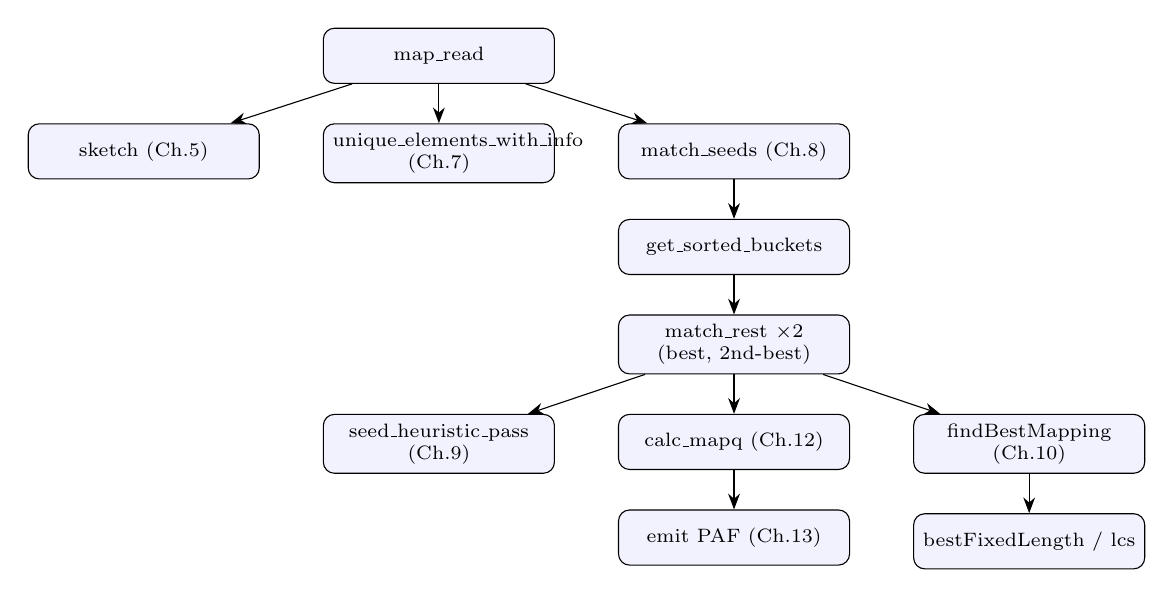
\begin{tikzpicture}[
    node distance=5mm and 8mm,
    every node/.style={font=\scriptsize},
    n/.style={draw, rounded corners, fill=blue!5, minimum height=7mm, text width=27mm, align=center},
    arr/.style={-{Stealth[length=2mm]}, thin}
  ]
  \node[n] (mr) {map\_read};
  \node[n, below left=of mr] (sketch) {sketch (Ch.5)};
  \node[n, below=of mr] (seed) {unique\_elements\_with\_info (Ch.7)};
  \node[n, below right=of mr] (ms) {match\_seeds (Ch.8)};
  \node[n, below=of ms] (gsb) {get\_sorted\_buckets};
  \node[n, below=of gsb] (mrest) {match\_rest $\times 2$ (best, 2nd-best)};
  \node[n, below left=of mrest] (shp) {seed\_heuristic\_pass (Ch.9)};
  \node[n, below right=of mrest] (fbm) {findBestMapping (Ch.10)};
  \node[n, below=of fbm] (score) {bestFixedLength / lcs};
  \node[n, below=of mrest] (mapq) {calc\_mapq (Ch.12)};
  \node[n, below=of mapq] (out) {emit PAF (Ch.13)};

  \draw[arr] (mr) -- (sketch);
  \draw[arr] (mr) -- (seed);
  \draw[arr] (mr) -- (ms);
  \draw[arr] (ms) -- (gsb);
  \draw[arr] (gsb) -- (mrest);
  \draw[arr] (mrest) -- (shp);
  \draw[arr] (mrest) -- (fbm);
  \draw[arr] (fbm) -- (score);
  \draw[arr] (mrest) -- (mapq);
  \draw[arr] (mapq) -- (out);
\end{tikzpicture}
\caption{Call graph of one \code{map\_read} invocation.}
\end{figure}

\section{Reference C++ implementation (annotated)}

\begin{lstlisting}[style=cppstyle,caption={\code{map\_read}, \texttt{src/shmap.h} --- core structure (elided: verbose-mode/diagnostic branches, identical in spirit to the pseudocode above)}]
inline void map_read(const params_t &params, const FracMinHash &sketcher,
                      ofstream &paulout, ofstream &unmapped_out,
                      const string &query_id, const string &P, BucketsType &B) {
    T.clear();
    B.clear();
    // NOTE: see Chapter 16 -- C.clear() is missing here in the reference source.

    sketch_t p = sketcher.sketch(P);
    qpos_t m = p.size();
    C.inc("read_len", P.size());

    Seeds p_unique = unique_elements_with_info(p);

    h2seed_t p_ht; h2cnt diff_hist; rpos_t possible_matches(0);
    for (const auto &kmer: p_unique) {
        p_ht.insert(make_pair(kmer.kmer.h, kmer));
        diff_hist[kmer.kmer.h] = kmer.occs_in_p;
        possible_matches += kmer.hits_in_T;
    }

    auto lmax = m;
    auto theta = params.theta;
    double theta2 = theta - params.min_diff;
    qpos_t S = qpos_t((1.0 - theta2) * m) + 1;

    if (abs_pos) B.set_halflen(P.size()); else B.set_halflen(m);

    match_seeds(p_unique, B, S);
    B.propagate_seeds_to_buckets();
    auto sorted_buckets = B.get_sorted_buckets();

    std::optional<Mapping> best, best2;
    best = match_rest(P.size(), m, lmax, p_unique, B, sorted_buckets, diff_hist, p_ht,
                       theta, std::nullopt, query_id, &lost_on_pruning, params.max_overlap);
    if (best) {
        double second_best_thr = best->score() * (1.0 - params.min_diff);
        best2 = match_rest(P.size(), m, lmax, p_unique, B, sorted_buckets, diff_hist, p_ht,
                            second_best_thr, best, query_id, &lost_on_pruning, params.max_overlap);
    }

    if (best) {
        if (best2) best->set_second_best(best2.value());
        os = &cout;
    } else {
        os = &unmapped_out;
    }
    // NOTE: see Chapter 16 -- the following two calls are unconditional in the reference
    // source even when `best` is empty; this listing shows the corrected, guarded form.
    best->set_global_stats(theta2, params.min_diff, m, query_id.c_str(), P.size(), params.k,
                            S, C.count("total_matches"), C.count("max_seed_matches"),
                            C.count("seed_matches"), C.count("seeded_buckets"),
                            C.count("final_buckets"), -1.0, T.secs("query_mapping"));
    best->print_paf(*os);
}
\end{lstlisting}

\chapter{Mapping Quality Estimation}
\label{ch:mapq}

\section{Inputs}

By the time MAPQ is computed, a read has: a best \code{Mapping} with score $f_1 \in [0,1]$ and
signed same-strand-seed count $\sigma_1$; optionally a second-best \code{Mapping} with score
$f_2 \le f_1$ (via \code{set\_second\_best}, below); and the run parameters $\theta_2$ (best-minus-
min\_diff threshold, \S\ref{sec:map-read}) and $\mathit{min\_diff}$ (CLI \code{-d}).

\section{\code{set\_second\_best}}

\begin{algobox}{title={\code{Mapping::set\_second\_best}(m2)}}
\begin{verbatim}
self.bucket2        := m2.bucket
self.intersection2  := m2.intersection
self.score2         := m2.score()
self.sigmas_diff    := sigmas_diff(self.intersection2, self.intersection)

function sigmas_diff(X, Y):
    X := (X == -1) ? 0 : X            # sentinel "no second best" reads as 0
    Y := (Y == -1) ? 0 : Y
    return abs(X - Y) / sqrt(X + Y)
\end{verbatim}
\end{algobox}

\code{sigmas\_diff} is a diagnostic-only quantity (emitted as the \code{Isdiff:f:} PAF tag,
\S\ref{ch:output}): treating the intersection counts as approximately Poisson-distributed, $|X-Y|
/\sqrt{X+Y}$ is the familiar ``number of standard deviations apart'' statistic for a difference of
two counts with variance $\approx$ their sum --- a quick, cheap significance proxy for how
distinguishable the best and second-best candidates' match counts are. It does not feed into
\code{calc\_mapq} itself.

\section{\code{calc\_mapq}: the concrete formula}
\label{sec:calc-mapq-formula}

\begin{algobox}{title={\code{Mapping::calc\_mapq}($\theta_2$, min\_diff)}}
\begin{verbatim}
if score2 < theta2:
    score2 := theta2                       # clamp: treat "no real 2nd best" as if it were theta2
frac := 1 - score2 / score()
# integer division on purpose -- see note below
mapq_strand := (abs(same_strand_seeds) < intersection / 2) ? 5 : 60
if frac > min_diff:
    return min(60, mapq_strand)
else:
    return 0
\end{verbatim}
\end{algobox}

\paragraph{Reading the formula.} Two independent signals are combined:
\begin{enumerate}
  \item \textbf{Score separation:} $\mathit{frac} = 1 - f_2/f_1$ (using the second-best score, or
    $\theta_2$ if there was no real second-best candidate or it scored below $\theta_2$). Large
    $\mathit{frac}$ means the best candidate is far ahead of any rival --- confident. The
    threshold for ``confident enough'' is exactly \code{min\_diff} (CLI \code{-d}): the same
    parameter that also sizes the seed budget (\S\ref{sec:seed-budget}) and the second-best
    search's own acceptance threshold (\S\ref{sec:match-rest}) is reused here as the MAPQ
    confidence cutoff too.
  \item \textbf{Strand consistency:} \code{same\_strand\_seeds} is the best mapping's own signed
    codirection tally (\S\ref{sec:type-match}); if fewer than half the matched $k$-mers agree with
    the reported strand (i.e., the mapping's own internal evidence for its stated orientation is
    weak), the achievable MAPQ is capped at $5$ rather than $60$, regardless of how good the score
    separation is.
\end{enumerate}
If $\mathit{frac} > \mathit{min\_diff}$: report $\min(60, \mathit{mapq\_strand})$ --- i.e., either
$60$ (confident, strand-consistent) or $5$ (confident on score alone, but strand-ambiguous). If
$\mathit{frac} \le \mathit{min\_diff}$: report $0$ unconditionally (not confident) --- notice this
is an \textbf{all-or-nothing} step function, not a smooth gradient between $0$ and $60$.

\begin{notebox}
The integer division \code{intersection / 2} in the strand-consistency check is exactly that ---
integer, truncating division, since \code{intersection} is stored as a 32-bit integer type in the
reference implementation. A from-scratch implementation that instead computes this comparison
using floating-point division will disagree with the reference for odd-valued
\code{intersection} counts (e.g.\ \code{intersection=5}: integer division gives $5/2=2$, so
\code{same\_strand\_seeds}$\,=2$ evaluates as \emph{not} $<2$, hence \code{mapq\_strand}$=60$;
floating-point division gives $2.5$, and $2 < 2.5$ evaluates true, hence \code{mapq\_strand}$=5$
--- a different MAPQ result for the identical input). Preserve integer truncation here.
\end{notebox}

\section{Two commented-out alternative formulas}

The reference source retains, directly above the live formula and clearly disabled (C++
\code{//} comments), two alternative MAPQ schemes:

\begin{enumerate}
  \item A ratio-based scheme using $\mathit{frac} = (1-f_2)/(1-f_1)$ with three tiers (full
    confidence above a threshold, zero below half that threshold, linear interpolation in
    between) --- a smoothly graduated version of the same idea, closer in spirit to minimap2's own
    published MAPQ formula ($40(1-f_2/f_1)\min(1,m/10)\log f_1$, referenced in a comment directly
    above these alternatives).
  \item A difference-based scheme using $\mathit{diff} = f_1 - f_2$ directly (rather than a ratio),
    with the same three-tier linear-interpolation structure.
\end{enumerate}
Their presence, never deleted, alongside the currently-live all-or-nothing formula, is evidence
of active, unfinished tuning rather than a settled design; a from-scratch implementation aiming
purely to reproduce shmap's \emph{shipped} behavior should implement only the live formula given
in \S\ref{sec:calc-mapq-formula} above, but an implementation aiming to \emph{improve} on it might
reasonably start from these alternatives (or from minimap2's own published formula) instead ---
this is flagged as a design choice, not a defect, since no test or shipped behavior depends on
which of the three is used going forward.

\section{Reference C++ implementation}

\begin{lstlisting}[style=cppstyle,caption={\code{Mapping::calc\_mapq}, \texttt{src/sketch.h} (live formula; the two commented-out alternatives immediately precede it in the source and are omitted here)}]
int calc_mapq(double theta2, double min_diff) {
    if (score2() < theta2) set_score2(theta2);
    double frac = 1.0 - score2()/score();
    int mapq_strand = (abs(local_stats.same_strand_seeds) < local_stats.intersection/2) ? 5 : 60;
    if (frac > min_diff) {
        return std::min(60, mapq_strand);
    } else {
        return 0;
    }
}
\end{lstlisting}

\section{When is \code{calc\_mapq} actually invoked}

Exactly once per \emph{mapped} read, from inside \code{Mapping::set\_global\_stats}
(\S\ref{sec:map-read-output}), \emph{after} \code{set\_second\_best} has already been called if a
second-best candidate exists (so that \code{score2()} reflects it) --- if no second-best was
found at all, \code{score2()} remains at its default sentinel ($-1.0$), which the clamp
\code{if (score2() < theta2) set\_score2(theta2)} converts into exactly $\theta_2$ before the
ratio is computed, giving a well-defined, maximally-confident result for uniquely-mapping reads
without any special-casing needed in the formula itself.

\chapter{Output Format}
\label{ch:output}

shmap emits one line per \emph{mapped} read to standard output, in an extended PAF format:
12 mandatory tab-separated PAF columns, followed by a long tail of \code{name:type:value}
optional tags in the SAM-style convention (\code{type} one of \code{i} integer, \code{f} float,
\code{s} string). Unmapped reads are written, one per line, to a separate \code{.unmapped.paf}
file (only created at all if an output prefix was configured, CLI \code{-z}).

\section{The 12 mandatory PAF columns}

\begin{center}
\begin{tabular}{@{}cllp{6.6cm}@{}}
\toprule
\# & Column & Source field & Meaning \\
\midrule
1 & query name & \code{query\_id} & Read id (FASTA header, truncated at first whitespace). \\
2 & query length & \code{p\_sz} & Read length in nucleotides. \\
3 & query start & \code{p\_start} & Always $0$ (shmap does not clip/trim the query side). \\
4 & query end & \code{p\_end} & Always \code{p\_sz}$-1$ under the current implementation --- see
  the note below; effectively always the full read length. \\
5 & strand & \code{strand} & \code{+} if the mapping's \code{same\_strand\_seeds} tally is
  positive, \code{-} otherwise. \\
6 & target name & \code{segm\_name} & Reference segment name (FASTA header). \\
7 & target length & \code{segm\_sz} & Reference segment length in nucleotides. \\
8 & target start & \code{t\_l} & Leftmost matched reference nucleotide position. \\
9 & target end & \code{t\_r} & Rightmost matched reference nucleotide position. \\
10 & \# matches & \code{p\_sz} (!) & See defect note below --- this column is supposed to be the
  actual residue-match count but instead always repeats the query-length column. \\
11 & block length & \code{p\_sz} (!) & Same defect: supposed to be the alignment block length,
  instead repeats query length. \\
12 & mapping quality & \code{mapq} & Chapter~\ref{ch:mapq}'s output, $\{0,5,60\}$ (or $255$ for
  ``not yet computed'', never actually observed in emitted output). \\
\bottomrule
\end{tabular}
\end{center}

\begin{bugbox}
Columns 10 and 11 (``number of residue matches'' and ``alignment block length'' in the PAF
specification) are, in the reference source, both hardcoded to repeat column 2 (query length)
rather than reporting the mapper's own computed intersection/span --- marked with a
\code{// TODO: fix} comment in the source itself. A from-scratch implementation aiming for a
\emph{spec-conformant} PAF file (e.g.\ for compatibility with downstream tools that read these
columns meaningfully, such as coverage calculators) should populate column 10 with the mapping's
\code{intersection} count and column 11 with its matched span (\code{t\_r - t\_l + 1}); one aiming
purely to reproduce shmap's own shipped output byte-for-byte should keep the repeated-query-length
placeholder.
\end{bugbox}

\section{Custom diagnostic tags (mapped reads)}

Appended, in this exact order, after the 12 mandatory columns. All tags below are always present
on every mapped-read output line (none are conditional).

\subsection{Per-candidate tags (\code{LocalMappingStats})}

\begin{center}
\begin{tabular}{@{}llp{8.6cm}@{}}
\toprule
Tag & Type & Meaning \\
\midrule
\code{p:i:} & int & Sketch size ($m$) considered for this read. \\
\code{s:i:} & int & Matched reference span (nucleotides or sketch-index units, per
  \code{abs\_pos}). \\
\code{I:i:} & int & Best mapping's intersection (matched $k$-mer) count. \\
\code{I2:i:} & int & Second-best mapping's intersection count ($-1$ sentinel if none). \\
\code{Idiff:i:} & int & \code{I} $-$ \code{I2} (note: if \code{I2} is the $-1$ sentinel, this is
  \code{I}$-(-1)=$\code{I}$+1$, \emph{not} \code{I}, since the raw sentinel value --- not the
  ``treat as 0'' convention used by \code{sigmas\_diff}, \S\ref{ch:mapq} --- is used directly
  here). \\
\code{Isdiff:f:} & float & \code{sigmas\_diff(I2, I)} (\S\ref{ch:mapq}; here the $-1\to0$
  convention \emph{does} apply, since it's computed by that function). \\
\code{J:f:} & float & Best mapping's score (whichever metric was selected, CLI \code{-m}). \\
\code{J2:f:} & float & Second-best score ($-1$ sentinel if none, \emph{not} clamped to $\theta_2$
  here --- that clamping is a side effect specific to \code{calc\_mapq}'s own internal
  computation, and by the time \code{calc\_mapq} runs it has already mutated \code{J2} in place,
  so in practice this tag \emph{does} show the clamped value whenever a MAPQ was computed with no
  real second-best; only relevant if reimplementing without that in-place mutation). \\
\code{Jdiff:f:} & float & \code{J} $-$ \code{J2}. \\
\code{sh:f:} & float & The seed-heuristic value ($h_{\mathrm{seed}}$, \S
  \ref{sec:seed-heuristic-theory}) at the moment this bucket was accepted. \\
\code{strand:i:} & int & \code{same\_strand\_seeds} signed tally (\S\ref{sec:type-match}). \\
\code{t:f:} & float & Wall-clock seconds spent mapping this read (never reproducible run-to-run;
  exclude when diffing output against a golden/reference file). \\
\code{b:s:} & string & Best mapping's bucket location, formatted \code{(segm\_id,b)}. \\
\code{b2:s:} & string & Second-best's bucket location, or the sentinel \code{(-1,-1)}
  (\S\ref{sec:type-bucketloc}) if none. \\
\bottomrule
\end{tabular}
\end{center}

\subsection{Run-wide/per-read summary tags (\code{GlobalMappingStats})}

\begin{center}
\begin{tabular}{@{}llp{8.6cm}@{}}
\toprule
Tag & Type & Meaning \\
\midrule
\code{k:i:} & int & $k$-mer length used (CLI \code{-k}). \\
\code{gt\_J:f:}, \code{gt\_C:f:}, \code{gt\_C\_bucket:f:} & float & Ground-truth
  Jaccard/containment fields --- \textbf{always} $-1.0$; declared and printed but never actually
  computed anywhere in the reference source (the real ground-truth comparison output is the
  entirely separate \code{-v~2} tag block, \S\ref{sec:ground-truth}, not these three). Kept as
  permanent $-1.0$ placeholders for output-format fidelity. \\
\code{seeds:i:} & int & Seed budget $S$ actually used for this read (\S\ref{sec:seed-budget}). \\
\code{max\_seed\_matches:i:} & int & Largest \code{hits\_in\_t} among any seed consumed this read.
\\
\code{seed\_matches:i:} & int & Total reference hits examined while matching seeds this read. \\
\code{total\_matches:i:} & int & Same as \code{seed\_matches:i:} at present (both are incremented
  together in \code{match\_seeds}; kept as two separately-named counters for forward
  compatibility with a scheme that might one day count additional non-seed matches separately). \\
\code{match\_inefficiency:f:} & float & \code{total\_matches / intersection} --- how many
  candidate-match examinations were needed per $k$-mer that actually ended up in the reported
  mapping; a rough proxy for how much the seed heuristic saved (lower is better; the reference
  tool's own runtime warning system, \S\ref{sec:runtime-warnings}, flags a run where this ratio
  implies the heuristic isn't earning its keep). \\
\code{seeded\_buckets:i:} & int & Distinct buckets touched by \code{match\_seeds} this read. \\
\code{final\_buckets:i:} & int & Buckets that survived pruning \emph{and} beat the running
  threshold at least once during \code{match\_rest} (counted across \emph{both} the best- and
  second-best search passes). \\
\code{FPTP:f:} & float & Always $-1.0$ --- a false-discovery-rate calculation that exists in the
  source as a fully commented-out, never-invoked function (\code{calc\_FDR}); kept as a permanent
  placeholder for the same reason as \code{gt\_J}/\code{gt\_C} above. \\
\bottomrule
\end{tabular}
\end{center}

\section{Ground-truth diagnostic tags (\code{-v 2} only)}
\label{sec:ground-truth}

When run with \code{-v~2} against \emph{simulated} reads whose FASTA header encodes the true
origin (format: \emph{anything}\code{!}\emph{segment\_name}\code{!}\emph{start}\code{!}
\emph{end}\code{!}\emph{strand}, e.g.\ \texttt{S1\_21!NC\_060948.1!57693539!57715501!+} --- exactly
5 \code{!}-separated fields), an additional block of tags is appended, and (if an output prefix
was configured) a parallel, more detailed TSV file (\code{<prefix>.paul.tsv}) is written, one row
per read, both mapped and unmapped.

\begin{center}
\begin{tabular}{@{}llp{8.4cm}@{}}
\toprule
Tag & Type & Meaning \\
\midrule
\code{gt\_segm:s:} & string & True segment name (parsed from the read name). \\
\code{gt\_start\_nucl:i:}, \code{gt\_end\_nucl:i:} & int & True start/end nucleotide positions
  (parsed from the read name). \\
\code{bucket\_l:i:} & int & This read's bucket half-length $\ell$. \\
\code{gt\_b\_l:s:}, \code{gt\_b\_r:s:}, \code{gt\_b\_next:s:} & string & The three buckets
  straddling the true position: one half-length before, at, and one half-length after
  $\lfloor \mathit{start}/\ell\rfloor$. \\
\code{gt\_M\_l:i:}, \code{gt\_M\_r:i:}, \code{gt\_M\_next:i:} & int & Number of (seed, hit) matches
  collected in each of those three buckets. \\
\code{gt\_J\_l:f:}, \code{gt\_J\_r:f:}, \code{gt\_J\_next:f:} & float & Best included-Jaccard
  score (\S\ref{sec:matcher-best-fixed-length}) achievable in each of those buckets, restricted to
  windows near the true span's length. \\
\code{gt\_C\_l:f:}, \code{gt\_C\_r:f:}, \code{gt\_C\_next:f:} & float & Best containment score in
  each, using the (dead-parameter, see Chapter~\ref{ch:defects}) ground-truth
  \code{bestFixedLength}. \\
\code{gt\_C\_l\_lmax:f:} & float & Numerically identical to \code{gt\_C\_l:f:} --- both call sites
  pass different values for a parameter the callee never reads (Chapter~\ref{ch:defects}). \\
\code{gt\_C\_r\_lmax:f:} & float & \textbf{Always} $-1.0$: declared, printed, but never assigned
  in the constructor at all (a distinct defect from the \code{gt\_C\_l\_lmax} redundancy above ---
  this one is a genuinely missing assignment, not a no-op parameter). \\
\bottomrule
\end{tabular}
\end{center}

The parallel \code{.paul.tsv} file additionally reports, per read: the count of buckets whose
included-Jaccard / containment score clears $\theta$ at all (\code{\#J>theta}, \code{\#C>theta}),
a bracketed listing of exactly which buckets those are with their individual scores
(\code{J>theta}, \code{C>theta}), the maximum score seen across all buckets
(\code{maxJ}, \code{maxC}), and the read's own raw sequence (\code{P}, the final column) --- this
file is intended for offline analysis of pruning/scoring quality against known-correct answers,
not for routine use.

\section{Unmapped-read record}
\label{sec:unmapped-record}

Per the fix recorded in Chapter~\ref{ch:defects}/\ref{ch:end-to-end}, an unmapped read is written
as a minimal, well-defined 12-column PAF-shaped line (broadly following the samtools/minimap2
convention for ``no alignment''):
\[
  \texttt{query\_id}\ \ \texttt{read\_len}\ \ 0\ \ 0\ \ \texttt{*}\ \ \texttt{*}\ \ 0\ \ 0\ \ 0\ \
  0\ \ 0\ \ 0
\]
i.e., query name and length populated, strand and target name as \code{*} (unknown), every other
numeric field zero. No diagnostic tags are appended for unmapped reads (there is no candidate
mapping to describe). This record is only ever written to the \code{.unmapped.paf} file
described above, which itself is only created when an output prefix (CLI \code{-z}) is given.

\section{Run-wide summary printed to stderr}
\label{sec:runtime-warnings}

At the end of a run, three human-readable reports are printed to standard error (never standard
output, so they never interleave with PAF data): (1) per-read averages/percentages for
kmer/match/bucket counts, mirroring the \code{GlobalMappingStats} tag definitions above but
aggregated across the whole run; (2) a timing breakdown (seconds and percentage-of-total spent in
each pipeline stage, plus a ``range ratio'' = slowest read / fastest read for that stage, useful
for spotting pathological reads); and (3) a short list of heuristic warnings (highlighted in
color) triggered when: fewer than 95\% of reads mapped; \code{match\_inefficiency} implies the
seed heuristic isn't paying for itself (average possible-matches-to-total-matches ratio below
10$\times$); more reads got \code{mapq=60} than \code{mapq=0} is \emph{violated} (i.e.\ a warning
fires when low-confidence mappings outnumber high-confidence ones); or any single pipeline stage
(seed matching, refinement, or specifically the second-best search within refinement) consumes
an outsized share of total runtime. These are operational/performance diagnostics, not part of
the mapping algorithm proper, and are safe to omit or reshape freely in a from-scratch
implementation.

\chapter{Command-Line Parameter Reference}
\label{ch:cli}

\begin{longtable}{@{}p{1.1cm}p{2.6cm}p{1.6cm}p{2.6cm}p{7cm}@{}}
\toprule
\textbf{Flag} & \textbf{Name} & \textbf{Default} & \textbf{Validation} & \textbf{Effect} \\
\midrule
\endfirsthead
\toprule
\textbf{Flag} & \textbf{Name} & \textbf{Default} & \textbf{Validation} & \textbf{Effect} \\
\midrule
\endhead
\code{-p} & pattern (reads file) & --- (required) & must exist & Path to the query reads,
  FASTA/FASTQ, optionally gzip-compressed. \\
\code{-s} & text (reference file) & --- (required) & must exist & Path to the reference,
  FASTA, optionally compressed. \\
\code{-k} & ksize & 15 & $>0$ & $k$-mer length, Chapter~\ref{ch:sketching}. \\
\code{-r} & hashratio & 0.05 & $(0,1]$ & FracMinHash keep-fraction $r$, \S
  \ref{sec:fracminhash-theory}. \\
\code{-S} & max\_seeds & unset & $>0$ if given & \textbf{Dead/inert}: parsed, validated, and
  printed in the parameter dump, but never read by any algorithmic code path (confirmed by
  exhaustive cross-reference). Kept for CLI compatibility only. \\
\code{-M} & max\_matches & unset (no cap) & $>0$ if given & Caps reference occurrences per $k$-mer
  hash before indexing, \S\ref{sec:max-matches}. \\
\code{-t} & threshold & 0.9 & $[0,1]$ & Acceptance threshold $\theta$, used throughout seeding
  (\S\ref{sec:seed-budget}) and refinement (\S\ref{sec:match-rest}). \\
\code{-d} & min\_diff & 0.02 & $\ge 0$ & $\mathit{min\_diff}$: MAPQ confidence cutoff
  (\S\ref{ch:mapq}), second-best search threshold factor (\S\ref{sec:match-rest}), and an input to
  the seed-budget formula (\S\ref{sec:seed-budget}) --- one parameter, three distinct uses. \\
\code{-o} & max\_overlap & 0.5 & $[0,1]$ & Overlap fraction above which a second-best candidate is
  rejected as a restatement of the best, \S\ref{sec:overlap-exclusion}. \\
\code{-m} & metric & Containment & one of \{Containment, Jaccard, bucket\_SH, bucket\_LCS\} &
  Selects the refinement scoring function, \S\ref{sec:metric-axis},
  Chapter~\ref{ch:scoring}. \\
\code{-z} & params (output prefix) & unset & --- & If set: (1) parameters are written to
  \texttt{<prefix>} as TSV instead of a human-readable dump to stderr; (2) unmapped reads are
  written to \texttt{<prefix>.unmapped.paf} (\S\ref{sec:unmapped-record}); (3) if \code{-v~2} is
  also set, ground-truth rows are written to \texttt{<prefix>.paul.tsv}
  (\S\ref{sec:ground-truth}). \\
\code{-v} & verbose & 0 & $\{0,1,2\}$ & $0$: silent. $1$: reserved (no distinct behavior beyond
  0 found). $2$: enables the ground-truth diagnostic path, \S\ref{sec:ground-truth} --- requires
  reads whose FASTA headers are ground-truth-encoded; using \code{-v~2} on ordinary reads is a
  usage error (the ground-truth parser will reject the header format; a from-scratch
  implementation should surface this as a clear error rather than the reference's own
  undefined/crashing behavior on malformed input in this mode). \\
\code{-n} & normalize & false & --- & \textbf{Dead/inert}: same status as \code{-S} --- parsed,
  printed, never read. \\
\code{-P} & no\_bucket\_pruning & false & --- & Disables seed-heuristic pruning entirely,
  \S\ref{sec:seed-heuristic-pass}. \\
\code{-B} & one\_sweep & false & --- & In the reference source: parsed and templated but
  \emph{never branched on anywhere in the mapper} --- fully dead despite having a descriptive
  help string (``disregards seed heuristic and runs one sweep on all matches''). This document's
  companion re-implementation gives it a concrete, best-effort meaning (consume every seed rather
  than the budget-limited $S$, \S\ref{sec:seed-budget}) since it was asked to make all
  configuration combinations real; see Chapter~\ref{ch:defects} for the full discussion and why
  this is explicitly a judgment call rather than a recovered original behavior. \\
\code{-F} & abs\_pos & false & --- & Selects nucleotide-position vs.\ sketch-index-position
  coordinate space for bucket/window arithmetic throughout Chapters~\ref{ch:bucketing}--
  \ref{ch:scoring}. \\
\code{-a} & sam & false & --- & \textbf{Dead/inert}, and additionally the entire SAM/CIGAR output
  code path this flag would have selected is itself fully commented out in the reference source
  (it depends on an edit-distance library that is otherwise unused). A from-scratch
  implementation targeting only the mapping functionality this document describes should not
  implement this flag at all. \\
\bottomrule
\caption{Every shmap CLI parameter, its validation rule, and its actual (not merely documented)
effect.}
\end{longtable}

\section{Parameters not exposed on the CLI but referenced throughout this document}

\begin{center}
\begin{tabularx}{\textwidth}{@{}llX@{}}
\toprule
\textbf{Symbol} & \textbf{Derived from} & \textbf{Defined in} \\
\midrule
$\theta_2$ & $\theta - \mathit{min\_diff}$ & \S\ref{sec:seed-budget}, \S\ref{sec:map-read} \\
$S$ (seed budget) & $\theta_2$, read sketch size $m$ & \S\ref{sec:seed-budget} \\
$\ell$ (bucket half-length) & read sketch size $m$ (or read length, if \code{abs\_pos}) &
  \S\ref{sec:bucket-halflen} \\
$\ell_{\min}$ & hardcoded constant, $5$ & \S\ref{sec:bucket-halflen} \\
\bottomrule
\end{tabularx}
\end{center}

\chapter{Complexity Analysis}
\label{ch:complexity}

Notation: $n$ = total reference length (nucleotides); $r$ = FracMinHash keep-fraction (\code{-r});
$|P|$ = one read's length; $m = |\hat P| \approx r|P|$ = its sketch size; $S\le m$ = seed budget
actually consumed (\S\ref{sec:seed-budget}); $d$ = a consumed seed's reference-hit count (capped
by \code{-M} when set, \S\ref{sec:max-matches}); $u$ = number of distinct buckets touched by one
read; $N$ = number of reads.

\section{Indexing (once per run)}

\begin{center}
\begin{tabularx}{\textwidth}{@{}llX@{}}
\toprule
\textbf{Step} & \textbf{Time} & \textbf{Space} \\
\midrule
Sketch every segment (Ch.\ 5) & $O(n)$ & $O(rn)$ (the kept $k$-mers) \\
Populate \code{h2single}/\code{h2multi} (Ch.\ 6) & $O(rn)$ amortized & $O(rn)$ \\
Sort each multi-hit list (Ch.\ 6) & $O\!\left(\sum_h d_h \log d_h\right) \le O(rn \log d_{\max})$
  & in place \\
\bottomrule
\end{tabularx}
\end{center}
Total: $O(n + rn\log d_{\max})$ time, $O(rn)$ space, independent of the number of reads that will
subsequently be mapped.

\section{Per read}

\begin{center}
\begin{tabularx}{\textwidth}{@{}llX@{}}
\toprule
\textbf{Step} & \textbf{Time} & \textbf{Notes} \\
\midrule
Sketch the read (Ch.\ 5) & $O(|P|)$ & \\
Group into seeds (Ch.\ 7) & $O(m\log m)$ & two sorts of size $m$ \\
Match seeds into buckets (Ch.\ 8) & $O(S\cdot \bar d)$ & $\bar d$ = avg.\ hit count of a consumed
  seed, $\le$ \code{-M} cap \\
Sort/dedup touched buckets (Ch.\ 8) & $O(u\log u)$ & $u\ll n/\ell$ in practice \\
Seed-heuristic pruning (Ch.\ 9) & $O(u)$ amortized, typically $O(1)$ per pruned bucket & see
  discussion below \\
Refine surviving buckets (Ch.\ 10) & $O(\ell)$ per surviving bucket & $\ell$ = bucket half-length
  $\approx m$ \\
MAPQ (Ch.\ 12) & $O(1)$ & \\
Emit PAF line (Ch.\ 13) & $O(1)$ & \\
\bottomrule
\end{tabularx}
\end{center}

\paragraph{Why pruning is (empirically) sublinear in the number of candidate buckets.} The
seed-heuristic bound (\S\ref{sec:seed-heuristic-theory}) only needs a bucket's running
\code{(seeds, matches)} counters, and tightens monotonically as more seeds are examined. In the
common case where a repetitive genome generates many candidate buckets but only one (or a
handful) is the true origin, every wrong bucket accumulates ``known misses'' quickly (most
consumed seeds simply do not have a reference hit inside a wrong bucket's span), so its bound
drops below $\theta$ after only a small, effectively $O(1)$-in-practice number of extension steps
--- this is an empirical/probabilistic claim (it depends on the genome's repeat structure and
$\theta$), not a worst-case guarantee: an adversarial input (e.g.\ a reference consisting almost
entirely of one repeated motif) can force every bucket to survive many extension rounds before
being resolved, degrading toward the $O(u \cdot m)$ worst case of exhaustively extending every
bucket with every seed.

\paragraph{Total per-read cost.} Combining the above, and noting $u$ is typically small relative
to $n/\ell$ (only a minority of possible bucket positions are ever touched by any real read's
seeds), a read's total mapping cost is, in the typical case, dominated by $O(m\log m)$ (seeding)
plus $O(\ell)$ (refining the eventual winner and perhaps a few near-misses) --- i.e.\
\textbf{roughly independent of total reference size $n$} once the index is built, which is
exactly the scaling property that makes sketch-based mapping practical at genome scale. Over $N$
reads: $O\bigl(n + rn\log d_{\max} + N(m\log m + \ell)\bigr)$ total.

\section{Memory}

Peak memory is dominated by the index: $O(rn)$ for the stored per-segment sketches
(\code{RefSegment.kmers}) plus $O(rn)$ for the hash maps (\code{h2single}/\code{h2multi}, one
entry per kept $k$-mer occurrence, with \code{h2multi} paying a small constant-factor overhead
per entry for its vector-of-hits indirection). Per-read working memory (seed table,
\code{diff\_hist}, touched-bucket list) is $O(m + u)$ and is released (or reused, in the
reference/port's actual implementation, which clears rather than reallocates,
\S\ref{sec:buckets-clear}) between reads, so it does not accumulate across a run.

\section{Practical scaling knobs}

\begin{center}
\begin{tabularx}{\textwidth}{@{}llX@{}}
\toprule
\textbf{Parameter} & \textbf{Increasing it\ldots} & \textbf{\ldots trades against} \\
\midrule
\code{-r} (keep fraction) & more sensitivity (finds weaker true matches) & linearly more index
  memory, more seeds per read, more refinement work per bucket \\
\code{-k} ($k$-mer length) & fewer spurious matches (larger alphabet space per $k$-mer) & more
  reads/regions missed entirely if error rate $\times k$ approaches 1 \\
\code{-t} (threshold $\theta$) & fewer accepted mappings, smaller seed budget $S$ & lower recall
  in genuinely divergent regions \\
\code{-M} (max\_matches cap) & fewer index entries scanned per common $k$-mer & silently drops
  legitimate signal from extremely repetitive true loci once capped \\
\bottomrule
\end{tabularx}
\end{center}

\chapter{Catalog of Defects and Dead Code in the Reference Implementation}
\label{ch:defects}

Every entry below was found during an exhaustive, function-by-function cross-reference of the
reference C++ source against an independent re-implementation, and confirmed either by
constructing a triggering test case or by an exhaustive grep-based call-site audit (for
dead-code claims: a claim of ``zero call sites'' means every reference to the symbol in the
entire source tree was individually inspected). None of these were assumed from documentation or
comments alone.

\section{Summary table}

\begin{center}
\begin{tabular}{@{}p{0.6cm}p{3.6cm}p{2.2cm}p{2.1cm}p{5.2cm}@{}}
\toprule
\# & \textbf{Defect} & \textbf{Affects live output?} & \textbf{Severity} & \textbf{Recommended
  handling} \\
\midrule
D1 & Uninitialized LUT arrays & Only non-ACGT input & Latent UB & Zero-initialize (\S
  \ref{sec:d1}) \\
D2 & \code{kmers\_notmatched} miscount & Diagnostic only & Cosmetic & Reorder the increment (\S
  \ref{sec:d2}) \\
D3 & \code{more\_seeds\_if\_cheap} unreachable & No (dead) & None & Optional to wire in (\S
  \ref{sec:d3}) \\
D4 & Hardcoded 100-segment cap & Crashes on $>100$ contigs & Usability & Size dynamically (\S
  \ref{sec:d4}) \\
D5 & \code{Buckets::size()} dead stub & No (dead) & None & Drop (\S\ref{sec:d5}) \\
D6 & \code{Mapping::do\_overlap} dead & No (dead) & None & Drop (\S\ref{sec:d6}) \\
D7 & \code{Matcher::do\_overlap}/\newline\code{lost\_correct\_mapping} dead & No (dead) & None &
  Drop (\S\ref{sec:d7}) \\
D8 & Dead \code{lmax} parameter in ground-truth \code{bestFixedLength} & Diagnostic only &
  Cosmetic/confusing & Drop the parameter (\S\ref{sec:d8}) \\
D9 & Off-by-one in \code{bestIncludedJaccard} & Diagnostic only (\code{-v 2}) & \textbf{Real
  correctness bug} & Fix indexing (\S\ref{sec:d9}) \\
D10 & Missing bounds clamp in ground-truth \code{collect\_matches} & Diagnostic only, potential
  crash/OOB & Latent bug & Clamp to segment length (\S\ref{sec:d10}) \\
D11 & \code{RefSegment::seq} unused waste & No (memory only) & Efficiency & Omit field (\S
  \ref{sec:d11}) \\
D12 & Dead \code{-a}/SAM output path & No (dead) & None & Omit entirely (\S\ref{sec:d12}) \\
D13 & Dead \code{-S}/\code{-n} CLI flags & No (dead) & None & Keep parsed-but-inert for
  compatibility (\S\ref{sec:d13}) \\
D14 & \code{one\_sweep}/\code{-B} never branched on & No (dead) & Usability/API honesty &
  Implement a concrete meaning (\S\ref{sec:d14}) \\
D15 & \textbf{Per-read counters never reset} & \textbf{Yes --- live PAF tags} & \textbf{Real
  correctness bug} & Fully reset every read (\S\ref{sec:d15}) \\
D16 & \textbf{Unconditional dereference of empty optional} & \textbf{Yes --- crashes/UB on every
  unmapped read} & \textbf{Real correctness bug (UB)} & Emit a defined minimal record (\S
  \ref{sec:d16}) \\
D17 & \code{gt\_C\_r\_lmax} never assigned & Diagnostic only (\code{-v 2}) & Cosmetic & Leave
  unassigned or compute it properly (\S\ref{sec:d17}) \\
D18 & PAF columns 10/11 always repeat query length & \textbf{Yes, if spec-conformance matters} &
  Cosmetic/compat & Populate real values if spec conformance is required (\S\ref{sec:d18}) \\
D19 & \code{Timers::secs}'s try/catch never catches anything & No (silent no-op) & Latent & Handle
  missing keys directly (\S\ref{sec:d19}) \\
D20 & \code{ParsedQueryId::parse} catches then rethrows & No & Style only & Simplify (\S
  \ref{sec:d20}) \\
\bottomrule
\end{tabular}
\end{center}

\section{D1: Uninitialized hash lookup tables}
\label{sec:d1}
\textbf{Location:} \code{FracMinHash} construction, \texttt{src/sketch.h} (\S\ref{sec:sketch-lut}).
\textbf{Description:} \code{LUT\_fw}/\code{LUT\_rc} are fixed 256-entry arrays; only the 8 entries
for \texttt{ACGTacgt} are ever written. Any other input byte (most commonly \texttt{N}) reads
uninitialized memory when used as a hash contribution --- undefined behavior in C++, and not even
a fixed garbage value (it depends on prior stack contents at the time \code{sketch()} first runs).
\textbf{Trigger:} any reference or read sequence containing a non-ACGT byte.
\textbf{Fix:} zero-initialize both tables before filling in the 8 real entries. This is a strict
safety improvement with zero behavioral change on ACGT-only input (the overwhelming majority of
real data), and was adopted without further discussion in the companion re-implementation.

\section{D2: \code{kmers\_notmatched} always reports the full sketch size}
\label{sec:d2}
\textbf{Location:} \code{unique\_elements\_with\_info}, \texttt{src/shmap.h} (\S
\ref{sec:seeding-grouping}). \textbf{Description:} the increment
\code{if (hits\_in\_t > 0) nonzero += strike;} is placed textually after \code{strike} has
already been reset to 0 for the next group, so it always adds zero; \code{kmers\_notmatched} (a
diagnostic counter only) therefore always reports the entire sketch size regardless of actual
match rate. \textbf{Impact:} cosmetic only --- feeds one end-of-run percentage in the stderr
summary (\S\ref{sec:runtime-warnings}), nothing else. \textbf{Fix:} move the increment before the
reset (or reorder the two statements).

\section{D3: \code{more\_seeds\_if\_cheap} is fully implemented but unreachable}
\label{sec:d3}
\textbf{Location:} \texttt{src/shmap.h} (\S\ref{sec:seed-budget}). \textbf{Description:} a
complete, presumably-tested function to opportunistically extend the seed budget when the next
seeds are (almost) unique in the reference; its only call site in \code{map\_read} is commented
out. \textbf{Impact:} none on shipped behavior (never runs). \textbf{Recommendation:} a
from-scratch implementation may wire it in (a plausible, low-risk recall improvement) or omit it
to match shipped behavior exactly; either is defensible.

\section{D4: Hardcoded 100-segment cap}
\label{sec:d4}
\textbf{Location:} \code{Buckets} construction, \texttt{src/buckets.h} (\S\ref{sec:buckets-struct}).
\textbf{Description:} \code{MAX\_SEGMENTS = 100}; construction throws for references with more
segments. \textbf{Trigger:} draft/scaffolded assemblies with hundreds or thousands of small
contigs --- not a rare input in practice. \textbf{Fix:} size the per-segment bucket storage to the
reference's actual segment count.

\section{D5--D7: Dead stubs and unreachable methods}
\label{sec:d5}
\label{sec:d6}
\label{sec:d7}
Three separate pieces of code are fully defined but have \textbf{zero} call sites anywhere in the
source tree (verified exhaustively, not just ``no obvious caller''):
\begin{itemize}
  \item \code{Buckets::size()} (\texttt{src/buckets.h}) --- literally \code{return -1;} with a
    \code{// TODO: implement} comment.
  \item \code{Mapping::do\_overlap} (\texttt{src/sketch.h}) --- a boolean overlap check,
    superseded everywhere by the (used) \code{Mapping::overlap} that returns a fraction
    (\S\ref{sec:overlap-exclusion}).
  \item \code{Matcher::do\_overlap} and \code{Matcher::lost\_correct\_mapping}
    (\texttt{src/refine.h}) --- ground-truth-overlap-checking helpers, superseded by the
    \code{-v 2} diagnostic path (\S\ref{sec:ground-truth}) actually used.
\end{itemize}
\textbf{Recommendation:} omit all three from a from-scratch implementation; they contribute no
behavior.

\section{D8: Dead \code{lmax} parameter in the ground-truth \code{bestFixedLength}}
\label{sec:d8}
\textbf{Location:} \texttt{src/refine.h}, the \code{Matcher}-scoped \code{bestFixedLength}
(\S\ref{sec:matcher-best-fixed-length}). \textbf{Description:} the function signature accepts an
\code{lmax} parameter, and every call site dutifully computes and passes a value for it
(\code{2*bucket\_l} or \code{bucket\_l}), but the function body's actual window-width check uses
\code{P\_sz} instead --- a commented-out \code{lmax}-based condition sits directly above the live
one, evidence the author switched approaches and left the now-ornamental parameter (and its
call-site computation) in place. \textbf{Consequence:} the two ground-truth tags
\code{gt\_C\_l\_lmax} and \code{gt\_C\_l} (\S\ref{sec:ground-truth}), whose call sites differ only
in what they pass for this dead parameter, are numerically \emph{identical} in practice.
\textbf{Fix:} drop the parameter; it does nothing.

\section{D9: Off-by-one in \code{bestIncludedJaccard} (real bug)}
\label{sec:d9}
\textbf{Location:} \texttt{src/refine.h}, \code{Matcher::bestIncludedJaccard}
(\S\ref{sec:matcher-best-fixed-length}). Full technical description already given in
\S\ref{sec:defect-prevr}; repeated here for completeness of this catalog. \textbf{Description:}
the function's window-growing loop scores mid-iteration using the position \emph{one before} the
just-processed element (\code{prev(r)}) for the reported span, while \code{intersection} at that
point already reflects the just-processed element --- an internal inconsistency that can and does
produce \code{intersection > span}, violating the metric's own $[0,1]$-boundedness invariant. The
original source carries an explicit \code{// TODO: should it be prev(r) instead?} comment on this
exact line. \textbf{Trigger:} confirmed via a small constructed example (a $\sim$50bp read against
a $\sim$200bp synthetic reference, exercising the \code{-v 2} ground-truth ``included Jaccard''
computation). \textbf{Impact:} affects only the \code{-v 2} diagnostic tags/TSV, never the primary
PAF output or any mapping decision (this sweep is not used by the main scoring path,
\S\ref{sec:best-fixed-length}, which has the analogous computation \emph{and gets it right} by
scoring only after its inner loop fully exits). \textbf{Fix:} score using the \emph{current},
just-processed right-boundary element consistently (matching what \code{intersection} already
counts), not the one before it.

\section{D10: Missing bounds clamp in ground-truth \code{collect\_matches}}
\label{sec:d10}
\textbf{Location:} \texttt{src/refine.h}, \code{Matcher::collect\_matches}. \textbf{Description:}
this function computes a bucket's \code{[start, end)} range into a segment's sketch array but does
not clamp \code{end} to the segment's actual length --- for the last bucket of a segment, a
bucket's nominal end can run past the sketch array's bounds, risking an out-of-bounds read. The
same file's own (separately dead, D7) \code{do\_overlap} function \emph{does} apply exactly this
clamp for the same quantity, suggesting the omission here is an oversight rather than intentional.
\textbf{Fix:} clamp \code{end} to \code{min(end, len(segment.kmers))} before iterating, mirroring
the clamp already present elsewhere in the same file.

\section{D11: \code{RefSegment::seq} is stored but never read (in the shipped feature set)}
\label{sec:d11}
\textbf{Location:} \texttt{src/sketch.h} (\S\ref{sec:type-refsegment}). \textbf{Description:} the
full raw nucleotide sequence of every reference segment is retained in memory, but the only code
that ever reads it (a SAM-output/edit-distance feature) is entirely commented out and
unreachable. For large references this is a substantial, unnecessary memory cost (roughly doubling
index memory beyond the sketch itself). \textbf{Recommendation:} omit the field entirely in a
from-scratch implementation targeting the mapping functionality this document describes; only
retain it if also implementing base-level alignment output.

\section{D12: Dead \code{-a}/SAM output path}
\label{sec:d12}
\textbf{Location:} CLI parsing (\texttt{src/io.h}) and \texttt{src/sketch.h}.
\textbf{Description:} the \code{-a} flag (\code{sam}) is parsed and stored but never read by any
live code; the SAM-format output function it would have selected is fully commented out (and
itself depends on an edit-distance library, \code{edlib}, that is otherwise entirely unused by the
shipped binary). \textbf{Recommendation:} omit this flag from a from-scratch implementation rather
than reproduce a no-op switch.

\section{D13: Dead \code{-S}/\code{-n} CLI flags}
\label{sec:d13}
\textbf{Location:} CLI parsing (\texttt{src/io.h}). \textbf{Description:} \code{max\_seeds}
(\code{-S}) and \code{normalize} (\code{-n}) are parsed, range-validated, and included in the
parameter dump, but neither is ever read by any algorithmic code. \textbf{Distinction from D12:}
unlike \code{-a}, these are not accompanied by a larger commented-out feature --- they appear to be
either forward-looking placeholders or remnants of a removed feature. \textbf{Recommendation:}
unlike the confirmed-and-explicitly-flagged \code{-a} case, a from-scratch implementation should
by default \emph{keep} these as accepted-but-inert CLI parameters (for command-line compatibility
with existing scripts/pipelines that may already pass them) rather than unilaterally removing
CLI-visible surface area that wasn't specifically identified for removal.

\section{D14: \code{one\_sweep}/\code{-B} has no implemented behavior}
\label{sec:d14}
\textbf{Location:} template parameter and CLI flag threaded throughout \texttt{src/shmap.h},
\texttt{src/mapper.cpp}. \textbf{Description:} unlike \code{no\_bucket\_pruning}/\code{-P} (which
does gate real behavior, \S\ref{sec:seed-heuristic-pass}) or \code{abs\_pos}/\code{-F} (which
gates coordinate-space arithmetic throughout Chapters~\ref{ch:bucketing}--\ref{ch:scoring}),
\code{one\_sweep} is threaded through every relevant function signature and even given a
descriptive CLI help string (``disregards seed heuristic and runs one sweep on all matches''), but
is never once tested inside any conditional in the mapper's actual logic --- confirmed via
exhaustive grep. \textbf{Recommendation:} since this document's companion implementation was
tasked with making every configuration combination genuinely meaningful (rather than silently
inert), it defines a concrete best-effort semantics matching the flag's own help text: consume
\emph{every} seed (\code{S := len(seeds)}) rather than the theta-derived budget
(\S\ref{sec:seed-budget}), leaving the rest of the pipeline (bucket pruning, refinement)
unchanged. This is an explicit design choice filling a gap the reference source left open, not a
recovered original behavior --- a from-scratch implementation is free to define \code{one\_sweep}
differently (e.g.\ literally skip bucket-based clustering and score one global sweep over every
raw match, which is closer to a literal reading of the help text but a substantially larger
undertaking) as long as it documents which interpretation it chose.

\section{D15: Per-read counters are never actually reset (real bug, affects live output)}
\label{sec:d15}
\textbf{Location:} \code{map\_read}, \texttt{src/shmap.h} (\S\ref{sec:map-read-counters}).
\textbf{Description:} the call that would fully reset the per-read \code{Counters} object
(\code{C.clear()}) is commented out; the subsequent re-initialization only names a subset of the
counter keys the function goes on to increment. The following counters are left unreset across
every read a single mapper instance processes: \code{read\_len}, \code{total\_matches},
\code{possible\_matches}, \code{kmers\_sketched}, \code{kmers\_unique}, \code{kmers\_seeds},
\code{seeded\_buckets}. Because the (also unreset) running counters object is merged into the
run-wide totals \emph{after every single read}, these specific counters compound
super-linearly across a run. \textbf{Concretely affected live output:} \code{total\_matches:i:}
and its derived \code{match\_inefficiency:f:} PAF tag (\S\ref{ch:output}) are read \emph{directly}
from this same, never-reset counters object \emph{before} the end-of-read merge into run-wide
totals --- meaning every mapped read's own reported \code{total\_matches:i:} value already
reflects leftover accumulation from every previous read the same mapper instance processed, not
just the current read. This is the most consequential defect in this catalog: it corrupts an
observable, per-mapping output field, not merely an end-of-run summary statistic.
\textbf{Confirmed} by observing, in a controlled two-read test, \code{total\_matches:i:} values
that were consistent per-read only after applying the fix below; without it, the second read's
value visibly incorporated the first read's contribribution. \textbf{Fix:} fully clear the
per-read counters object at the start of every read, and pre-register (at zero) every counter
name the function's call graph touches (the complete, corrected list is: every name in the
reference source's own partial list, \emph{plus} the seven listed above).

\section{D16: Unconditional dereference of an empty optional on unmapped reads (real bug, UB)}
\label{sec:d16}
\textbf{Location:} \code{map\_read}, \texttt{src/shmap.h} (\S\ref{sec:map-read-output}).
\textbf{Description:} \code{best->set\_global\_stats(...)} and \code{best->print\_paf(...)} are
called unconditionally, textually after the point where the code has already branched on whether
\code{best} holds a value or not --- for every unmapped read, this dereferences an empty
\code{std::optional<Mapping>}, which is undefined behavior in C++ (it does not reliably crash;
depending on standard-library internals it may silently read whatever a default-constructed-
looking object's memory layout happens to contain). \textbf{Trigger:} any read that does not map
(a normal, expected, frequently-occurring outcome --- the surrounding code clearly anticipates it,
since a dedicated \code{unmapped\_out} stream and \code{lost\_on\_seeding}/\code{lost\_on\_pruning}
counters all exist specifically to track this case). \textbf{Fix:} guard both calls behind the
same \code{if (best)} check already present a few lines above, and define an explicit,
well-formed output for the unmapped case instead --- this document's companion implementation
writes a minimal 12-column PAF-shaped record (\S\ref{sec:unmapped-record}) rather than silently
omitting unmapped reads from output entirely, on the reasoning that the reference source's own
\code{unmapped\_out} stream was clearly intended to receive \emph{some} record per unmapped read,
even though the bug above meant it never cleanly did.

\section{D17: \code{gt\_C\_r\_lmax} is declared, printed, but never assigned}
\label{sec:d17}
\textbf{Location:} \code{AnalyseSimulatedReads} constructor, \texttt{src/analyse\_simulated.h}
(\S\ref{sec:ground-truth}). \textbf{Description:} distinct from D8 (which is a dead
\emph{parameter}) --- this is a genuinely missing assignment. The constructor computes and stores
\code{gt\_C\_l\_lmax} but has no corresponding \code{gt\_C\_r\_lmax = ...} line at all, despite
both fields being declared and both being unconditionally printed in \emph{both} the \code{-v 2}
PAF tags and the \code{.paul.tsv} output. \textbf{Impact:} the \code{gt\_C\_r\_lmax:f:} tag / TSV
column always shows the default \code{Mapping}'s sentinel score, $-1.000$, for every read, in
every run. \textbf{Recommendation:} since this diagnostic path has zero automated test coverage
to indicate the intended value, a from-scratch implementation may either leave the field
unassigned (matching shipped behavior exactly) or assign it the obviously-analogous computation
(mirroring \code{gt\_C\_l\_lmax} but for the right-side ground-truth bucket) --- both are
defensible; this document's companion implementation chose to leave it unassigned, to avoid
inventing behavior for a code path with no oracle to validate against.

\section{D18: PAF columns 10/11 always repeat the query-length column}
\label{sec:d18}
Already described in full in \S\ref{ch:output}; included here for completeness of this catalog.
Marked with the reference source's own \code{// TODO: fix} comment.

\section{D19: \code{Timers::secs}'s exception handling can never actually fire}
\label{sec:d19}
\textbf{Location:} \texttt{src/utils.h}. \textbf{Description:} \code{Timers::secs(name)} wraps
\code{timers\_.at(name).secs()} in a \code{try \{ ... \} catch (const std::runtime\_error\&)}
intended to gracefully handle a missing timer name. However, \code{std::unordered\_map::at} throws
\code{std::out\_of\_range} on a missing key, which does \emph{not} derive from
\code{std::runtime\_error} in the C++ standard exception hierarchy (both derive independently from
\code{std::exception}) --- so this catch clause can never actually trigger for the failure mode it
was written for. In practice this is masked because every timer name actually queried has always
been previously \code{.start()}'d (which auto-vivifies the entry), so the missing-key path is
never exercised by the shipped tool. \textbf{Recommendation:} a from-scratch implementation should
simply handle the ``timer not found'' case directly (e.g.\ return $0.0$ and log, which was
evidently the original intent) rather than reproduce a try/catch that provides no actual safety
net.

\section{D20: \code{ParsedQueryId::parse} catches a parse error only to rethrow it}
\label{sec:d20}
\textbf{Location:} \texttt{src/utils.h}. \textbf{Description:} when a ground-truth-encoded read
name's numeric fields (start/end position) fail to parse as integers, the function catches the
resulting exception, logs an error message, sets a (about-to-be-discarded) validity flag to false,
and then rethrows the same exception unconditionally --- so the net behavior is identical to not
catching it at all, just with an extra log line first. \textbf{Distinction from the two graceful
cases the same function handles} (no \code{!}-delimiter present at all; wrong number of
\code{!}-delimited fields), both of which \emph{do} return a clean ``not a ground-truth name''
result: a malformed \emph{numeric} field within an otherwise correctly-shaped name is treated as a
hard failure, not a graceful ``not ground-truth-encoded'' result. \textbf{Recommendation:}
this is reasonable, defensible behavior for a diagnostic feature that assumes well-formed
simulated-read names (only used in the opt-in \code{-v 2} mode); a from-scratch implementation
should simply let the parse error propagate (panic/exception) without the pointless
catch-log-rethrow wrapper, since the wrapper adds a log message but changes nothing else.

\appendix
\chapter{Notation, Glossary, and Quick Index}
\label{ch:appendix}

\section{Notation summary}

\begin{center}
\begin{tabularx}{\textwidth}{@{}llX@{}}
\toprule
\textbf{Symbol} & \textbf{Meaning} & \textbf{Defined} \\
\midrule
$k$ & $k$-mer length & \S\ref{sec:sketch-lut}, CLI \code{-k} \\
$r$ & FracMinHash keep-fraction & \S\ref{sec:fracminhash-theory}, CLI \code{-r} \\
$H_{\max}$ & Maximum hash value ($2^{64}-1$) & \S\ref{sec:fracminhash-hash} \\
$n$ & Total reference length & \S\ref{ch:complexity} \\
$|P|$ & Read length (nucleotides) & \\
$m$ & Read's sketch cardinality & \S\ref{sec:seeding-grouping} \\
$S$ & Seed budget (occurrences) consumed & \S\ref{sec:seed-budget} \\
$\theta$ & Acceptance threshold & CLI \code{-t} \\
$\theta_2$ & $\theta - \mathit{min\_diff}$ & \S\ref{sec:seed-budget} \\
$\mathit{min\_diff}$ & MAPQ/threshold margin & CLI \code{-d} \\
$\ell$ & Bucket half-length & \S\ref{sec:bucket-halflen} \\
$\ell_{\min}$ & Minimum allowed $\ell$ ($=5$) & \S\ref{sec:bucket-halflen} \\
$h_{\mathrm{seed}}$ & Seed-heuristic bound & \S\ref{sec:seed-heuristic-theory} \\
$J(A,B)$ & Jaccard similarity & \S\ref{sec:minhash} \\
$C(A,B)$ & Containment index & \S\ref{sec:fracminhash-theory} \\
$f_1, f_2$ & Best / second-best mapping score & \S\ref{ch:mapq} \\
\bottomrule
\end{tabularx}
\end{center}

\section{Glossary}

\begin{description}[style=nextline,leftmargin=1.2cm]
\item[Bucket] A fixed-geometry, overlapping candidate window along one reference segment
  (Chapter~\ref{ch:bucketing}).
\item[Canonical $k$-mer] A $k$-mer identified by a strand-agnostic combination of its forward and
  reverse-complement hash (\S\ref{sec:canonical-kmers}).
\item[Containment index] Fraction of one set's elements found in another; shmap's primary scoring
  metric (\S\ref{sec:fracminhash-theory}).
\item[FracMinHash] A hash-threshold-based sketching scheme giving length-proportional sketch size
  (\S\ref{sec:fracminhash-theory}).
\item[Hit] A $k$-mer's occurrence in the \emph{reference} (\S\ref{sec:type-hit}).
\item[Jaccard similarity] Intersection over union of two sets (\S\ref{sec:minhash}).
\item[MAPQ] Mapping quality, a Phred-like confidence score for a reported mapping
  (\S\ref{sec:mapq-theory}, Chapter~\ref{ch:mapq}).
\item[Minimizer] The smallest-hash $k$-mer in a sliding window; an alternative sketching scheme
  shmap does \emph{not} use (\S\ref{sec:minimizers}).
\item[PAF] Pairwise mApping Format, shmap's output format (Chapter~\ref{ch:output}).
\item[Rolling hash] An $O(1)$-amortized-update hash recurrence over sliding windows
  (\S\ref{sec:rolling-hash}).
\item[Seed] One distinct $k$-mer hash from a read's sketch, with reference/read occurrence
  metadata attached (\S\ref{sec:type-seed}).
\item[Seed heuristic] The closed-form pruning upper bound central to shmap's performance
  (\S\ref{sec:seed-heuristic-theory}, Chapter~\ref{ch:pruning}).
\item[Sketch] A subsampled representative subset of a sequence's $k$-mers
  (\S\ref{sec:minhash}--\S\ref{sec:fracminhash-theory}).
\end{description}

\section{Quick algorithm index}

\begin{center}
\begin{tabularx}{\textwidth}{@{}llX@{}}
\toprule
\textbf{Function} & \textbf{Section} & \textbf{Purpose} \\
\midrule
\code{sketch} & \S\ref{ch:sketching} & FracMinHash rolling hash \\
\code{build\_index} & \S\ref{ch:indexing} & Reference $k$-mer index \\
\code{unique\_elements\_with\_info} & \S\ref{sec:seeding-grouping} & Group read $k$-mers into
  seeds \\
\code{match\_seeds} & \S\ref{sec:match-seeds} & Populate buckets from the seed budget \\
\code{hseed} & \S\ref{ch:pruning} & Seed-heuristic bound formula \\
\code{seed\_heuristic\_pass} & \S\ref{sec:seed-heuristic-pass} & Incremental pruning loop \\
\code{bestFixedLength} (SHMapper) & \S\ref{sec:best-fixed-length} & Main Containment/Jaccard sweep
\\
\code{lcs} & \S\ref{sec:lcs-implementation} & bucket\_LCS metric \\
\code{findBestMapping} & \S\ref{sec:find-best-mapping} & Metric dispatch \\
\code{match\_rest} & \S\ref{sec:match-rest} & Best/second-best search \\
\code{calc\_mapq} & \S\ref{sec:calc-mapq-formula} & MAPQ formula \\
\code{map\_read} & \S\ref{sec:map-read} & Full per-read driver \\
\bottomrule
\end{tabularx}
\end{center}

\section{Minimal reference implementation checklist}

A from-scratch implementation is functionally complete once it has:
\begin{enumerate}[nosep]
  \item Bit-exact FracMinHash sketching (Chapter~\ref{ch:sketching}), verified via the
    reverse-complement symmetry test (end of \S\ref{ch:sketching}).
  \item A reference index with correct single/multi occurrence splitting and sorted multi-hit
    lists (Chapter~\ref{ch:indexing}).
  \item Rarest-first seed grouping with correctly-collected \code{pmatches} (Chapter~\ref{ch:seeding}).
  \item Overlapping bucket geometry with the 50\% overlap rule applied consistently
    (Chapter~\ref{ch:bucketing}).
  \item The seed-heuristic bound implemented and unit-tested against hand-derived examples
    (Chapter~\ref{ch:pruning}).
  \item All four scoring metrics (Chapter~\ref{ch:scoring}), each independently verified (e.g.\
    against a brute-force $O(n)$ containment/Jaccard computation on small synthetic inputs).
  \item Best/second-best search with overlap exclusion and MAPQ (Chapters~\ref{ch:end-to-end}--
    \ref{ch:mapq}).
  \item Well-defined (not undefined-behavior) handling of the unmapped case
    (\S\ref{sec:unmapped-record}).
  \item PAF output matching \S\ref{ch:output}'s column/tag definitions.
\end{enumerate}
Chapter~\ref{ch:defects} should be read in full before finalizing any of the above, since several
entries there materially change what ``correct'' means for a specific function relative to a
naive reading of the reference source alone.


\end{document}
